\section{LEAPR}
\label{sLEAPR}
\index{LEAPR|textbf}

\hypertarget{sLEAPRhy}{The}
LEAPR\index{LEAPR} module is used to prepare the scattering law
$S(\alpha,\beta)$\index{$S(\alpha,\beta)$}, which describes thermal
scattering\index{thermal scattering} from bound moderators, in the
ENDF-6 format used by
\hyperlink{sTHERMRhy}{THERMR}\index{THERMR}.  The original ENDF thermal
scattering data\cite{GAreport} was prepared by General Atomics (GA)
using the GASKET code\cite{GASKET}.  This code has difficulty working
with the very large energy and momentum transfers encountered for
large incident energy or very low temperatures.  For these reasons,
LEAPR is based on the British code LEAP+ADDELT originally written
by McLatchie\index{McLatchie} at Harwell\cite{McLatchie}, then
implemented by Butland\index{Butland} at Winfrith\cite{Butland},
and finally modified to work better for cold moderators as part of
the Ph.D. Thesis of D.~J.~Picton\cite{Picton}\index{Picton}.  The
code that Dr. Picton provided
was modified extensively to fit better into the NJOY environment
and to take advantage of modern large computers.  This involved
massive rearrangement of storage and routines, updating for first
FORTRAN-77,  then Fortran-90, and extensive editing of the comment
cards.  The original Edgewood expansion and Short Collision
Time (SCT) treatments were removed in favor of using more terms
in the phonon expansion and using the simple ENDF SCT
formula\cite{ENDF102}.\index{short collision time} In
addition, output in ENDF-6 format\cite{ENDF102} was provided, the
capability to include either coherent or incoherent elastic scattering
was added\index{coherent elastic}\index{incoherent elastic},  a major
speedup for the diffusion calculation was provided, and a capability
to produce a mixed scattering law for materials like BeO\index{BeO}
and benzine\index{benzine} was developed.  In order to improve the numerics
on short-word computers, the code was changed to use the asymmetric
scattering function, the normalization scheme for the phonon
expansion was revised, and the discrete-oscillator calculation
was rebuilt to take better advantage of the convolution properties
of the delta function and to use better Bessel Functions.  A complete
discussion of the theory used in the code is given below.

LEAPR was used\cite{New} to reevaluate several of the thermal moderator
materials from ENDF/B-VI\index{ENDF!ENDF/B-VI} using the original GA
physics\cite{GAreport} but extending the alpha and beta ranges for
incoherent inelastic\index{incoherent inelastic} scattering.  The
energy range for coherent scattering was also increased.  The code
was also used to prepare scattering-law files for several cold
moderators\index{cold moderators} of interest for experimental
cold-neutron sources\cite{ICANS,coldworkshop}.  More recently, some
of these materials were updated for ENDF/B-VII.0\index{ENDF!ENDF/B-VII}
and additional materials were added.  Several of the ENDF/B-VII.0 cases
are discussed below as examples of how to run LEAPR.

Acknowledgements are due to Gary Russell\index{Russell} of the
Los Alamos Neutron Science Center (LANSCE) for motivating this
work, to Drew Kornreich\index{Kornreich} of the University of Arizona
for his careful study of the water problem, and to Max Lazo\index{Lazo}
(University of New Mexico, SAIC, and Sandia National Laboratory) for
testing and reviewing the code and documentation.  In addition, we
thank D. J. Picton\index{Picton} for sending us his cold-moderator
version of LEAPR, Rolf Neef\index{Neef} of Julich and Guy
Robert\index{Robert} of ILL-Grenoble for sending us the initial
version of the cold hydrogen treatment, and M. Mattes\index{Mattes}
and J. Keinert\index{Keinert} of the University of Stuttgart for their
help with the liquid hydrogen and deuterium models.

This chapter describes the LEAPR module in NJOY2016.0.

\subsection{Theory}
\label{ssLEAPR_theory}

The following discussion of the theories used in the the code is based
on the original British documentation and the presentation in a standard
reference\cite{Parks}.


\paragraph{Coherent and Incoherent Scattering.}
In practice, the scattering of neutrons from a system of N particles
with a random distribution of spins or isotope types can be expressed
as the sum of a coherent part and an incoherent part.  The coherent
scattering includes the effects from waves that are able to interfere
with each other, and the incoherent part depends on a simple sum of
noninterfering waves from all the N particles.  (The spin correlations
in ortho and para hydrogen violate the assumption of randomness, so
liquid hydrogen\index{liquid hydrogen} does not fit into the model
described here.  A method for treating them will be described below.)
The cross sections for coherent and incoherent scattering can be
considered to be characteristic properties of the materials.
\index{coherent elastic}\index{incoherent elastic}  As examples,
the scattering from hydrogen is almost completely incoherent, and the
scattering from carbon and oxygen is almost completely coherent.

Furthermore, the coherent and incoherent scattering include both
elastic and inelastic parts.  The elastic scattering takes place with
no energy change.  It should not be confused with the elastic
scattering from a single particle that is familiar for higher neutron
energies where the neutron loses energy; thermal elastic scattering can
be considered to be scattering from the entire lattice, thus the
effective mass of the target is very large, and the neutron does not
lose energy in the scattering process.  Thermal inelastic scattering
results in an energy loss (gain) for the neutron with a corresponding
excitation (deexcitation) of the target.  The excitation may correspond
to the production of one or more phonons in a crystalline material, to
the production of rotations or vibrations in molecules, or to the
initiation of atomic or molecular recoil motions in a liquid or gas.

In addition, the coherent inelastic part of the scattering contains both
interference effects between waves scattered by different particles and
direct terms.  It turns out that the direct part for gases, liquids and
solids consisting of randomly oriented crystallites has approximately the
same form as the incoherent term.  The interference is usually neglected.

Therefore, we can usually divide the thermal scattering cross section into
three different parts:

\begin{itemize}
\begin{singlespace}
   \item {\it Coherent elastic.}  Important for crystalline solids
        like graphite or beryllium.\index{coherent elastic}

   \item {\it Incoherent elastic.} Important for hydrogenous solids
        like solid methane, polyethylene, and zirconium
        hydride.\index{incoherent elastic}

   \item {\it Inelastic.} Important for all materials
        (this category includes both incoherent and coherent
        inelastic).\index{incoherent inelastic}
\end{singlespace}
\end{itemize}

The absence of interference in incoherent scattering and the neglect of
interference in coherent inelastic scattering allows us to construct
thermal scattering laws for ``hydrogen in water" or ``hydrogen in
solid methane'' or ``oxygen in beryllium oxide".  However, this
simplification is not possible in general for coherent elastic scattering
in materials with more that one type of atom in the unit cell;
for coherent elastic scattering, beryllium oxide must be considered as
a unit.

\paragraph{Inelastic Scattering}
It is shown in the standard references\cite{Parks} that the double
differential scattering cross section for thermal neutrons for gases,
liquids or solids consisting of randomly ordered microcrystals can be
written as

\begin{equation}
   \sigma(E{\rightarrow}E',\mu)=\frac{\sigma_b}{2kT}
      \sqrt{\frac{E'}{E}}\,{\cal S}(\alpha,\beta)\,,
\end{equation}

\noindent
where $E$ and $E'$ are the incident and secondary neutron energies in the
laboratory system, $\mu$ is the cosine of the scattering angle in the
laboratory, $\sigma_b$ is the characteristic bound scattering cross
section for the material, $kT$ is the thermal energy in eV, and ${\cal S}$
is the asymmetric form of the scattering law.  The  scattering law depends
on only two variables: the momentum transfer

\begin{equation}
   \alpha=\frac{E'+E-2\mu\sqrt{E'E}}{AkT}\,,
\label{alph}
\end{equation}

\noindent
where $A$ is the ratio of the scatterer mass to the neutron mass, and
the energy transfer

\begin{equation}
   \beta=\frac{E'-E}{kT}\,.
\end{equation}

\noindent
Note that $\beta$ is positive for energy gain and negative for energy
loss.  Working in the incoherent approximation and the Gaussian approximation,
the scattering law\index{scattering law} can be written

\begin{equation}
   {\cal S}(\alpha,\beta)=\frac{1}{2\pi}\intall\exx{i\beta\hat{t}}
      \,\exx{-\gamma(\hat{t})}\,d\hat{t}\,,
   \label{sincoh}
\end{equation}

\noindent
where $\hat{t}$ is time measured in units of $\hbar/(kT)$ seconds.
The function $\gamma(\hat{t})$ is given by

\begin{equation}
   \gamma(\hat{t})=\alpha\intall P(\beta)
      \left[\,1-\exx{-i\beta\hat{t}}\,\right]\,\exx{-\beta/2}\,d\beta\,,
   \label{gamma}
\end{equation}

\noindent
where

\noindent
\begin{equation}
   P(\beta)=\frac{\rho(\beta)}{2\beta\sinh(\beta/2)}\,,
   \label{pbeta}
\end{equation}

\noindent
and where $\rho(\beta)$ is the frequency spectrum\index{frequency spectrum}
of excitations in the system expressed as a function of $\beta$.  The
spectrum must be normalized as
follows:

\begin{equation}
   \int_0^\infty \rho(\beta)\,d\beta=1\,.
   \label{rnorm}
\end{equation}

\noindent
The function $P(\beta)$ defined by Eq.(\ref{pbeta}) is used directly in
LEAPR, and $\rho(\beta)=\rho(\epsilon/kt)$ is given as a function of
$\epsilon$ in eV.  For systems in thermal equilibrium, there is a
relationship  between upscatter and downscatter called ``detail balance''
\index{detail balance} that is a consequence of microscopic reversibility.
 It requires that

\begin{equation}
  {\cal S}(\alpha,\beta)=\exx{-\beta}{\cal S}(\alpha,-\beta)\,.
\end{equation}

\noindent
Liquid hydrogen\index{liquid hydrogen} and deuterium violate this
condition, as will be described below.  In addition, the scattering
law satisfies two other important constraints; namely, normalization,

\begin{equation}
   \intall {\cal S}(\alpha,\beta)\,d\beta=1\,,
   \label{ssnorm}
\end{equation}

\noindent
and the sum rule

\begin{equation}
   \intall \beta\,{\cal S}(\alpha,\beta)\,d\beta=-\alpha\,.
   \label{sssum}
\end{equation}

\noindent
Actually, ENDF works with the so-called ``symmetric'' $S(\alpha,\beta)$,

\begin{equation}
   S(\alpha,\beta)=\exx{\beta/2}\,{\cal S}(\alpha,\beta)\,
\end{equation}

\noindent
which (except for liquid hydrogen or deuterium) satisfies the condition

\begin{equation}
   S(\alpha,\beta)=S(\alpha,-\beta)\,.
\end{equation}

\noindent
Note that ${\cal S}(\alpha,-\beta)$ for positive $\beta$ describes
the downscatter side of the function, and because it is basically
proportional to the cross section, it can be represented by reasonable
numbers (say $10^{-8}$ to 1) for all $\beta$.  The symmetric
$S(\alpha,\beta)$, on the other hand, can easily be smaller than ${\cal
S}(\alpha,-\beta)$ by factors like ${\rm e}^{-\beta/2} \sim {\rm e}^{-80}
\sim 10^{-35}$, which can cause trouble on short-word machines.
This kind of numerical problem is even more severe for cold moderators,
where dynamic ranges on the order of $10^{100}$ occur for
$S(\alpha,\beta)$.  (The user will have to use some caution reading this
report, because the typographic symbols for S and script-S are very
similar.)  By working with ${\cal S}(\alpha,-\beta)$, LEAPR can do all
of its calculations using single-precision variables, even on
a short-word machine.

The next step is to decompose the frequency spectrum into a sum of
simple spectra

\begin{equation}
   \rho(\beta)=\sum_{j=1}^K\rho_j(\beta),
\end{equation}
\vspace{0.5 pt}

\noindent
where the following possibilities are allowed:

\begin{eqnarray}
  \rho_j(\beta) &=& w_j\delta(\beta_j)\;\; \hbox{discrete oscillator}\\
  \rho_j(\beta) &=& \rho_s(\beta)  \;\;\;\; \hbox{solid-type spectrum}\\
  \rho_j(\beta) &=& \rho_t(\beta)  \;\;\;\; \hbox{translational spectrum}
\end{eqnarray}

\noindent
The solid-type spectrum must vary as $\beta^2$ as $\beta$ goes to zero,
and it must integrate to $w_s$, the weight for the solid-type law.  The
translational spectrum can be either a free-gas law or a diffusion-type
spectrum represented with the approximation of Egelstaff and Schofield
that will be discussed later.  In either case, the spectrum must
integrate to $w_t$, the translational weight.  The sum of all the
weights of the partial spectra must equal 1.  Defining
$\gamma_j(\hat{t})$ to be the value of $\gamma$ appropriate for
$\rho_j$, and ${\cal S}_j$ to be the corresponding partial scattering law,
and using the convolution theorem for Fourier transforms, leads to a
recursive formula for the scattering law:

\begin{equation}
   {\cal S}(\alpha,\beta)={\cal S}^{(K)}(\alpha,\beta),
\end{equation}

\noindent
where

\begin{eqnarray}
   {\cal S}^{(J)}(\alpha,\beta) &=&
      \frac{1}{2\pi}\intall\exx{i\beta\hat{t}}
      \prod_{j=1}^J\exx{-\gamma_j(\hat{t})}\,d\hat{t} \nonumber\\
     &=&\intall{\cal S}_J(\alpha,\beta')\,
        {\cal S}^{(J-1)}(\alpha,\beta{-}\beta')\,d\beta'\,.
\end{eqnarray}

\noindent
As an example of the use of this recursive procedure, consider a case
where the desired frequency spectrum is a combination of $\rho_s$ and
two discrete oscillators.  First, calculate ${\cal S}^{(1)}{=}{\cal
S}_1$ using $\rho_s$.  Then calculate ${\cal S}_2$ using
$\rho(\beta_1)$, the distribution for the first discrete oscillator,
and convolve ${\cal S}_2$ with ${\cal S}^{(1)}$ to obtain ${\cal
S}^{(2)}$, the composite scattering law for the first two partial
distributions.  Repeat the process with the second discrete oscillator
to obtain ${\cal S}^{(3)}$, which is equal to ${\cal S}(\alpha,\beta)$
for the full distribution.

\paragraph{The Phonon Expansion.}\index{phonon expansion} Consider
first $\gamma_s(\hat{t})$, the Gaussian function for solid-type
frequency spectra.  Expanding the time-dependent part of the exponential
gives

\begin{equation}
   \exx{-\gamma_s(\hat{t})}=\exx{-\alpha\lambda_s}
      \sum_{n=0}^{\infty}\frac{1}{n!}\left[\,\alpha
      \intall P_s(\beta)\,\exx{-\beta/2}\exx{-i\beta\hat{t}}
      \,d\beta\,\right]^n\,,
\end{equation}

\noindent
where $\lambda_s$ is the Debye-Waller coefficient

\begin{equation}
   \lambda_s=\intall P_s(\beta)\,\exx{-\beta/2}\,d\beta\,.
   \label{dbwf}
\end{equation}
\vspace{0.5 pt}

\noindent
The scattering function becomes

\begin{eqnarray}
   {\cal S}_s(\alpha,\beta)&=&\exx{-\alpha\lambda_s}\sum_{n=0}^{\infty}
      \frac{1}{n!}\alpha^n\nonumber\\
      & &\times\,\frac{1}{2\pi} \intall\exx{i\beta\hat{t}}\left[
      \intall P_s(\beta')\,\exx{-\beta'/2}\,\exx{-i\beta'\hat{t}}
      \,d\beta'\right]^n d\hat{t}\,.
\end{eqnarray}

\noindent
For convenience, define the quantity in the second line of this equation
to be $\lambda_s^n {\cal T}_n(\beta)$.  Then clearly,

\begin{equation}
   {\cal S}_s(\alpha,\beta)=\exx{-\alpha\lambda_s}
    \sum_{n=0}^{\infty}\frac{1}{n!}\,[\alpha\lambda_s]^n\,{\cal T}_n(\beta)\,,
   \label{phoexp}
\end{equation}

\noindent
where

\begin{equation}
   {\cal T}_0(\beta)=\frac{1}{2\pi}
      \intall\exx{i\beta\hat{t}}\,d\hat{t}=\delta(\beta)\,,
\end{equation}

\noindent
and

\begin{equation}
   {\cal T}_1(\beta)=\intall \frac{P_s(\beta')\,
      \exx{-\beta'/2}}{\lambda_s}\left\{\frac{1}{2\pi}
      \intall\exx{i(\beta{-}\beta')\hat{t}}\,d\hat{t}\right\}d\beta'
      =\frac{P_s(\beta)\,\exx{-\beta/2}}{\lambda_s}\,,
\end{equation}

\noindent
In general,

\begin{equation}
   {\cal T}_n(\beta)=\intall {\cal T}_1(\beta')\,
      {\cal T}_{n-1}(\beta{-}\beta')\,d\beta'\,.
   \label{phoconv}
\end{equation}

\noindent
The script-T functions obey the relationship
${\cal T}_n(\beta)=\exx{-\beta}{\cal T}_n(-\beta)$.
In addition, each of the ${\cal T}_n$ functions
obeys the following normalization condition:

\begin{equation}
   \intall {\cal T}_n(\beta)\,d\beta = 1\,.
\end{equation}

\noindent
It guarantees that Eq.\ref{ssnorm} will be satisfied by the sum in
Eq.\ref{phoexp}.  In LEAPR, the ${\cal T}_n(-\beta)$ functions are
precomputed on the input $\beta$ grid for $n$ up to some specified
maximum value, typically 100.  It is then easy to compute the smooth
part of ${\cal S}_s(\alpha,-\beta)$ for any sufficiently small value of
$\alpha$ using Eq.\ref{phoexp}.  The corresponding values of
${\cal S}_s(\alpha,\beta)$ can then be obtained by multiplying by
$\exx{-\beta}$.  The delta function arising from the ``zero-phonon''
term is carried forward separately.  The normalization in
Eq.\ref{phoexp} has better numerical properties than the one used in
LEAP.

\paragraph{The Short-Collision-Time Approximation.}\index{short collision time}
For larger values of $\alpha$, the expansion of Eq.\ref{phoexp} requires
too many terms.  LEAPR uses the simple Short-Collision-Time (SCT)
approximation from ENDF to extend the solid-type scattering law.

\begin{equation}
   {\cal S}_s(\alpha,-\beta)=\frac{1}{\sqrt{4\pi w_s\alpha
      \overline{T}_s/T}}\,
      \exp\left[-\frac{(w_s\alpha-\beta)^2}{w_s\alpha
      \overline{T}_s/T}\right]\,,
\end{equation}

\noindent
and

\begin{equation}
   {\cal S}_s(\alpha,\beta)=\exx{-\beta}{\cal S}_s(\alpha,-\beta)\,
\end{equation}

\noindent
where $\beta$ is positive, and
where the effective temperature\index{effective temperature} is given by

\begin{equation}
   \overline{T}_s = \frac{T}{2 w_s}
       \intall\beta^2 P_s(\beta)\,\exx{-\beta}\,d\beta\,.
\end{equation}

\noindent
As above, $w_s$ is the weight for the solid-type spectrum.

\paragraph{Diffusion and Free-Gas Translation.}
The neutron scattering from many important liquids, including water
and liquid methane, can be represented using a solid-type spectrum
of rotational and vibrational modes combined with a
diffusion\index{diffusion} term.  Egelstaff and Schofield have
proposed an especially simple model for diffusion called the
``effective width model''.  It has the advantage of having
analytic forms for both $S(\alpha,\beta)$ and the
associated frequency spectrum $\rho(\beta)$:

\begin{eqnarray}
   {\cal S}_t(\alpha,\beta)&=&\frac{2 c w_t\alpha}{\pi}\,
       \,\exp\left[2 c^2 w_t\alpha-\beta/2\right]\, \nonumber\\
     & &\frac{\sqrt{c^2+.25}}{\sqrt{\beta^2+4 c^2 w_t^2\alpha^2}}\,
     K_1\Bigl\{\sqrt{c^2+.25}\sqrt{\beta^2+4 c^2 w_t^2 \alpha^2}
     \Bigr\}\,,
\end{eqnarray}
\vspace{0.5 pt}

\noindent
and

\begin{equation}
   \rho(\beta)=w_t \frac{4 c}{\pi\beta}\,\sqrt{c^2+.25}\,
      \sinh(\beta/2)\,K_1\Bigl\{\sqrt{c^2+.25}\,\beta\Bigr\}\,.
\end{equation}
\vspace{0.5 pt}

\noindent
In these equations, $K_1(x)$ is a modified Bessel function of the
second kind, and the translational weight $w_t$ and the
diffusion constant $c$ are provided as inputs.

An alternative for the translational part of the distribution is
the free-gas law.\index{free gas}  It is clearly appropriate for
a gas of molecules, but it has also been used to represent the
translational component for liquid moderators like water\cite{GAreport}.
The scattering law is given by

\begin{equation}
   {\cal S}_t(\alpha,-\beta)=\frac{1}{\sqrt{4\pi w_t\alpha}}
       \,\exp\left[-\frac{(w_t\alpha-\beta)^2}{4w_t\alpha}\right]\,,
\end{equation}

\noindent
and

\begin{equation}
   {\cal S}_t(\alpha,\beta)=\exx{-\beta}{\cal S}_t(\alpha,-\beta)\,,
\end{equation}

\noindent
with $\beta$ positive.  The free-gas law is used in LEAPR if the
diffusion coefficient $c$ is input as zero.

In LEAPR, ${\cal S}_s(\alpha,\beta)$, the scattering law for the solid-type
modes, is calculated using the phonon expansion as described above.
The translational contribution ${\cal S}_t(\alpha,\beta)$ is then calculated
using one of the formulas above on a $\beta$ grid chosen to represent its
shape fairly well.  The combined scattering law is then obtained
by convolution as follows:

\begin{equation}
   {\cal S}(\alpha,\beta)={\cal S}_t(\alpha,\beta)\,\exx{-\alpha\lambda_s}
     +\intall {\cal S}_t(\alpha,\beta')\,
      {\cal S}_s(\alpha,\beta{-}\beta')\,d\beta'.
\end{equation}

\noindent
The first term arises from the delta function in Eq.\ref{phoexp},
which isn't included in the numerical results for the phonon series
calculation.  The values for ${\cal S}_t(\beta)$ and
${\cal S}_s(\beta{-}\beta')$ are obtained from
the precomputed functions by interpolation.  This makes LEAPR run
much faster than LEAP+ADDELT for diffusive cases, because the original
code did direct recalculations of the solid-type scattering law for
all the desired values of $\beta{-}\beta'$.  It also had to take pains
to compute $S_t$ on a $\beta$ grid that was commensurate with the
input grid.  This often resulted in more points for $S_t$ than were
necessary to obtain useful accuracy for the convolutions.

The effective temperature\index{effective temperature} for a
combination of solid-type and translation modes is computed using

\begin{equation}
   \overline{T}_s = \frac{w_t T + w_s \overline{T}_s}{w_t+w_s}\,.
\end{equation}

\paragraph{Discrete Oscillators.}\index{discrete oscillators}
Polyatomic molecules normally contain a number of vibrational
modes that can be represented as discrete oscillators.  The distribution
function for one oscillator is given by $w_i\delta(\beta_i)$, where
$w_i$ is the fractional weight for mode $i$, and $\beta_i$ is the
energy-transfer parameter computed from the mode's vibrational
frequency.  The corresponding scattering law is given by

\begin{eqnarray}
   {\cal S}_i(\alpha,\beta) &=& \exx{-\alpha\lambda_i}\sum_{n=-\infty}^\infty\,
     \delta(\beta-n\beta_i) \, I_n \left[
       \frac{\alpha w_i}{\beta_i\sinh(\beta_i/2)} \right]\,
         \exx{-n\beta_i/2}\nonumber\\
      & = & \sum_{n=-\infty}^\infty\,A_{in}(\alpha)\,
             \delta(\beta-n\beta_i)\,,
\end{eqnarray}

\noindent
where

\begin{equation}
   \lambda_i = w_i \frac{\coth(\beta_i/2)}{\beta_i}\,.
\end{equation}

\noindent
The combination of a solid-type mode (s) with discrete
oscillators (1) and (2) would give

\begin{eqnarray}
   {\cal S}^{(0)}(\alpha,\beta)&=&{\cal S}_s(\alpha,\beta)\,,\\
   {\cal S}^{(1)}(\alpha,\beta) &=& \intall {\cal S}_1(\alpha,\beta')\,
      {\cal S}^{(0)}(\alpha,\beta{-}\beta')\,d\beta' \nonumber\\
       &=& \sum_{n=-\infty}^\infty\,A_{1n}(\alpha)\,
        {\cal S}^{(0)}(\alpha,\beta{-}n\beta_1)\,,\\
    {\cal S}^{(2)}(\alpha,\beta)&=&\intall {\cal S}_2(\alpha,\beta')\,
       {\cal S}^{(1)}(\alpha,\beta{-}\beta')\,d\beta' \nonumber\\
      &=& \sum_{m=-\infty}^\infty\,A_{2m}(\alpha)\,
           \sum_{n=-\infty}^\infty\,A_{1n}(\alpha)\,\,
        {\cal S}^{(0)}(\alpha,\beta{-}n\beta_1{-}m\beta_2)\,.
\end{eqnarray}

\noindent
This process can be continued through ${\cal S}^{(3)}(\alpha,\beta)$,
${\cal S}^{(4)}(\alpha,\beta)$, etc., until all the discrete oscillators
have been included.  The result has the form

\begin{equation}
  {\cal S}(\alpha,\beta)=\sum_k W_k(\alpha)\,
          {\cal S}_s(\alpha,\beta-\beta_k)\,,
\end{equation}

\noindent
where the $\beta_k$ and the associated weights $W_k$ are easily
generated recursively using a procedure that throws out small weights
at each step.  The Debye-Waller $\lambda$ for the combined
modes is computed using

\begin{equation}
  \lambda=\lambda_s+\sum_{i=1}^N \lambda_i\,.
\end{equation}

\noindent
The effective temperature\index{effective temperature} for the
combined modes is given by

\begin{equation}
   \overline{T}_s=w_t T + w_s \overline{T}_s
    + \sum_{i=1}^N w_i \frac{\beta_i}{2}
     \coth\left(\frac{\beta_i}{2}\right) T\,.
\end{equation}

If the starting-point scattering law ${\cal S}^{(0)}$ does not contain
a translational contribution (true for hydrogenous solids like
polyethylene and frozen methane), it is important to remember to
include the effects of the ``zero-phonon'' term
$\exp(-\alpha\lambda_s)\delta(\beta)$.  The code does this by
adding in triangular peaks with the proper areas and with their apexes
at the $\beta$ value closest to the $\beta_k$ values.  One of these
peaks is at $\beta{=}0$.  This peak is not put into the scattering
law as a sharp triangle; instead, it is handled as
``incoherent elastic'' scattering in order to take full advantage of
the analytic properties of $\delta(\beta)$.

\paragraph{Incoherent Elastic Scattering.}\index{incoherent elastic}
In hydrogenous solids, there is an elastic (no energy loss) component of
scattering arising from the ``zero-phonon'', or $n{=}0$ term, of
Eq.\ref{phoexp}.  In ENDF terminology, this is called the ``incoherent
elastic'' term.
Clearly,

\begin{equation}
   S_{\rm iel}(\alpha,\beta)=\rm e^{-\alpha\lambda}\delta(\beta)\,.
\end{equation}

\noindent
The corresponding differential scattering cross section is

\begin{equation}
   \sigma(E,\mu)=\frac{\sigma_b}{2}\,\rm e^{-2WE(1-\mu)}\,,
\end{equation}

\noindent
and the integrated cross section is

\begin{equation}
   \sigma(E)=\frac{\sigma_b}{2}\left\{\frac{1-\rm e^{-4WE}}{2WE}\right\}\,.
\end{equation}

\noindent
In these equations, the Debye-Waller coefficient\index{Debye-Waller
coefficient} is given by

\begin{equation}
   W=\frac{\lambda}{AkT}\,,
\end{equation}

\noindent
where $\lambda$ is computed from the input frequency spectrum as shown
by Eq.\ref{dbwf} and modified by the presence of discrete
oscillators (if any) as shown above.  LEAPR writes the bound scattering
cross section $\sigma_b$ and the Debye-Waller coefficient $W$ as a
function of temperature into a section of the ENDF-6 output
with MF=7 and MT=2.

\paragraph{Coherent Elastic Scattering.}\index{coherent elastic}
In solids consisting of coherent scatterers -- for example, graphite -- the
zero-phonon term leads to interference scattering from the various planes
of atoms of the crystals making up the solid.  Once again, there is no
energy loss, and the ENDF term for the process is ``coherent elastic
scattering''.  The differential scattering cross section is given by

\begin{equation}
   \sigma_{\rm coh}(E,\mu)=\frac{\sigma_c}{E}
      \sum_{E_i<E}f_i\,\rm e^{-4WE_i}\delta(\mu-\mu_i)\,,
\end{equation}

\noindent
where

\begin{equation}
   \mu_i=1-E_i/E\,,
\end{equation}

\noindent
and the integrated cross section is given by

\begin{equation}
   \sigma_{\rm coh}=\frac{\sigma_c}{E}
      \sum_{E_i<E}f_i\,\rm e^{-4WE_i}.
   \label{coh1}
\end{equation}

\noindent
In these equations, $\sigma_c$ is the effective bound coherent scattering
cross section for the material, $W$ is the effective Debye-Waller coefficient,
$E_i$ are the so-called ``Bragg Edges'',\index{Bragg edges} and the
$f_i$ are related to the crystallographic structure factors.

It can be seen from Eq.\ref{coh1} that the coherent elastic cross section
is zero below the first Bragg Edge, $E_1$ (typically about 2 to 5 meV).  It
then jumps sharply to a value determined by $f_1$ and the Debye-Waller term.
At higher energies, the cross section drops off as $1/E$ until $E{=}E_2$.
It then takes another jump, and resumes its $1/E$ drop off.  The sizes
of the steps in the cross section gradually get smaller, and at high energies
there is nothing left but an asymptotic $1/E$ decrease (typically above
1 to 2 eV).  LEAPR stores the quantity $E\sigma_{\rm coh}(E)$ as a function
of energy and temperature in a section of the ENDF-6 output with MF=7 and
MT=2.  The cross section is easily recovered from this representation by
dividing by $E$ (this is done in the
\hyperlink{sTHERMRhy}{THERMR}\index{THERMR} module of NJOY).
The angular distribution of scattered neutrons can be calculated by
extracting the $f_i$ from the steps in $\sigma_{\rm coh}(E)$ file by
subtraction.  This process is carried out automatically in the
\hyperlink{sGROUPRhy}{GROUPR}\index{GROUPR} module of NJOY.

The calculation of the $E_i$ and $f_i$ depends on a knowledge of the
crystal structure of the scattering material.  The methods used are
borrowed from HEXSCAT\cite{HEXSCAT}.
In general, the energies of the Bragg edges are given by

\begin{equation}
   E_i=\frac{\hbar^2\tau_i^2}{8m}\,,
\end{equation}

\noindent
where $\tau_i$ is the length of the vectors of one particular ``shell''
of the reciprocal lattice, and $m$ is the neutron mass.  The $f_i$ factors
for a material containing a single atomic species are given by

\begin{equation}
   f_i=\frac{2\pi\hbar^2}{4mNV}\sum_{\tau_i} |F(\tau)|^2\,,
\end{equation}

\noindent
where the sum extends over all reciprocal lattice vectors of the given
length, and the crystallographic structure factor is given by

\begin{equation}
  |F(\tau)|^2=\Bigl|\sum_{j=1}^{N}\rm e^{i2\pi\phi_j}\Bigr|^2\,,
\end{equation}

\noindent
where $N$ is the number of atoms in the unit cell,
$\phi_j=\vec{\tau}\cdot\vec{\rho}_j$
are the phases for the atoms, and the $\vec{\rho}_j$ are their positions.
The situation is more complicated for materials containing different
atomic species, such as beryllium oxide.  In these cases,

\begin{equation}
   \sigma_c\rm e^{-2WE_i}f_i=\Bigl|\sum_{j=1}^{N}
      \sqrt{\sigma_j}\,\rm e^{-W_jE_i}\rm e^{i2\pi\phi_j}\Bigr|^2\,,
\end{equation}

\noindent
where the coherent cross section and Debye-Waller factor can be different
for each site in the unit cell.  The effective coherent cross section is
clearly given by

\begin{equation}
   \sigma_c=\sum_{j=1}^{N}\sigma_j\,.
\end{equation}

\noindent
Since LEAPR only works with one material at a time, it doesn't have access
to different values of $W_j$ for the atoms in the unit cell.  Therefore, it
assumes that either $W_jE_i$ is small, or the $W_j$ doesn't vary much from
site to site.  This allows it to calculate the $f_i$ using

\begin{equation}
   |F|^2=\Bigl|\sum_{j=1}^N\frac{\sqrt{\sigma_j}}{\sqrt{\sigma_c}}
      \,\rm e^{-2\pi\phi_j}\Bigr|^2\,.
\end{equation}
\vspace{0.5 pt}

\noindent
For hexagonal materials, the lattice is described by the two constants
$a$ and $c$.  The reciprocal lattice vector lengths are given by

\begin{equation}
   \Bigl(\frac{\tau}{2\pi}\Bigr)=\frac{4}{3a^2}
      \Bigl(\ell_1^2+\ell_2^2+\ell_1\ell_2\Bigr)
      +\frac{1}{c^2}\ell_3^2\,
\end{equation}
\vspace{0.5 pt}

\noindent
where $\ell_1,\ell_2,$ and $\ell_3$ run over all the positive and negative
integers, including zero.  The volume of the unit cell is

\begin{equation}
   V=\sqrt{3}a_2c/2\,.
\end{equation}

\noindent
For graphite, there are four atoms in the unit cell at positions\cite{Wycoff}
$$
   (0,0,0),\,(-\frac{1}{3},\frac{1}{3},0),\,
      (-\frac{2}{3},-\frac{1}{3},\frac{1}{2}),\,
        (-\frac{1}{3},\frac{1}{3},\frac{1}{2})\,.
$$

\noindent
These positions give the following phases:

\begin{eqnarray}
   \phi_1 &=& 0\,,\\
   \phi_2 &=& (-\ell_1+\ell_2)/3\,,\\
   \phi_3 &=& -(2/3)\ell_1-(1/3)\ell_2+(1/2)\ell_3\,,\\
   \phi_4 &=& -(1/3)\ell_1+(1/3)\ell_2+(1/2)\ell_3\,.
\end{eqnarray}

\noindent
The form factor for graphite becomes

\begin{equation}
   |F|^2=\left\{
     \begin{array}{ll}
        6+10\cos[2\pi(\ell_1-\ell_2)/3] & \mbox{$\ell_3$ even}\\
        4\sin^2[\pi(\ell_1-\ell_2)/3] & \mbox{$\ell_3$ odd}
     \end{array}
   \right.
\end{equation}
\vspace{0.5 pt}

\noindent
For the hexagonal close packed (hcp) structure, which includes beryllium,
there are two atoms per unit cell at
$$
   (0,0,0),\,(\frac{1}{3},\frac{2}{3},\frac{1}{2})\,,
$$

\noindent
and the form factor for hcp lattices like beryllium becomes

\begin{equation}
   |F|^2=2+2\cos\Bigl[2\pi(2\ell_1+4\ell_2+3\ell_3)/6\Bigr]\,.
\end{equation}
\vspace{0.5 pt}

The beryllium oxide lattice consists of two interpenetrating hcp lattices,
one for the beryllium atoms, and one for the oxygen.  There are four atoms
per unit cell with positions
$$
   (0,0,0),\,(\frac{1}{3},\frac{2}{3},\frac{1}{2}),\,
    (0,0,u), (\frac{1}{3},\frac{2}{3},u+\frac{1}{2})\,,
$$
\vspace{0.5 pt}

\noindent
Using the approximation that the Debye-Waller factor doesn't vary from
position to position in the unit cell gives the following expression for
the structure factor:
\begin{equation}
   |F|^2=\Bigl(1+\cos[2\pi(2\ell_1+4\ell_2+3\ell_3)/6]\Bigr)
      \Bigl(r_1^2+2r_1r_2\cos(3\pi\ell_3/4)\Bigr)\,,
\end{equation}

\noindent
where $r_1^2$ and $r_2^2$ are the bound coherent cross sections for
beryllium and oxygen, respectively, and the effective coherent cross
section, $\sigma_c$, is to be taken as 1.

LEAPR contains similar logic to handle face-centered cubic (fcc),
{\it e.g.} aluminum,
and body-centered cubic (bcc), {\it e.g.} iron, lattices.  More formulas
for the structure factor can be added to the code when needed.

\paragraph{Liquid Hydrogen and Deuterium.}\index{liquid hydrogen}
Materials containing hydrogen (H) or deuterium (D) molecules violate the
assumption that spins are distributed randomly that underlies the
incoherent approximation used for Eq.\ref{phoexp}, and an explicitly
quantum-mechanical formula is required to take account of the correlations
between the spins of two atoms in the same molecule.  This problem was
considered by Young and Koppel\cite{YK}.  Changing to our notation, the
formulas for the hydrogen molecule (neglecting vibrations) become

\begin{eqnarray}
    {\cal S}_{\rm para}(\alpha,\beta)&=&\sum_{J=0,2,4,\dots}P_J \nonumber \\
      &\times&\frac{4\pi}{\sigma_b}\Bigl[A_{\rm para}\sum_{J'=0,2,4,\dots}
       +B_{\rm para}\sum_{J'=1,3,5,\dots}\Bigr](2 J'+1)\nonumber\\
      &\times&{\cal S}_f(w\alpha,\beta{+}\beta_{JJ'})\nonumber\\
      &\times&\sum_{\ell=|J'-J|}^{J'+J}4\,j_\ell^2(y)\,C^2(JJ'\ell;00)\,,
\label{spara}
\end{eqnarray}

\noindent
and
\begin{eqnarray}
    {\cal S}_{\rm ortho}(\alpha,\beta)&=&\sum_{J=1,3,5,\dots}P_J\nonumber\\
      &\times&\frac{4\pi}{\sigma_b}\Bigl[A_{\rm ortho}\sum_{J'=0,2,4,\dots}
       +B_{\rm ortho}\sum_{J'=1,3,5,\dots}\Bigr](2 J'+1)\nonumber\\
      &\times&{\cal S}_f(w\alpha,\beta{+}\beta_{JJ'})\nonumber\\
      &\times&\sum_{\ell=|J'-J|}^{J'+J}4\,j_\ell^2(y)\,C^2(JJ'\ell;00)\,.
\label{sortho}
\end{eqnarray}

\noindent
The coefficients for the even and odd sums are given in the following table:

\begin{center}
\begin{tabular}{lcc}
Type  &  $A$(even)  &  $B$(odd) \\ \hline
H para  &  $a_c^2$  &  $a_i^2$ \\
H ortho  &  $a_c^2/3$  & $a_c^2+2a_i^2/3$ \\
D para  & $3a_i^2/4$  &  $a_c^2+a_i^2/4$ \\
D ortho  &  $a_c^2+5a_i^2/8$  &  $3a_i^2/8$ \\ \hline
\end{tabular}
\end{center}
\index{para hydrogen}
\index{ortho hydrogen}
\index{para deuterium}
\index{ortho deuterium}

\noindent
Here $a_c$ and $a_i$ are the coherent and incoherent scattering lengths
(note that the characteristic bound cross section is
$\sigma_b{=}4\pi[a_c^2{+}a_i^2]$), $P_J$ is the statistical weight
factor, $\beta_{JJ'}{=}(E_J'{-}E_J)/kT$ is the energy transfer for a
rotational transition, $j_\ell(x)$ is a spherical Bessel function of
order $\ell$, and $C(JJ'\ell;00)$ is a Clebsch-Gordan coefficient.
The parameter $y$ is given by $\kappa a/2{=}(a/2)\sqrt{4MkT\alpha/2}$,
where $a$ is the interatomic distance in the molecule. The translational
weight $w$ is 1/2 for H$_2$ and 1/4 for D$_2$.  The sums over $J'$ are
treated as operators into order to keep the notation compact.

Young and Koppel assumed that the molecular translations were
free,\index{free gas}
so the equations contain

\begin{equation}
   {\cal S}_f(\alpha,-\beta)=\frac{1}{\sqrt{4\pi\alpha}}
       \,\exp\left[-\frac{(\alpha-\beta)^2}{4\alpha}\right],
\end{equation}

\noindent
and

\begin{equation}
   {\cal S}_f(\alpha,\beta)=\rm e^{-\beta}{\cal S}_f(\alpha,-\beta)\,,
\end{equation}

\noindent
the free-atom scattering function (with $\beta$ positive).  Note that
$\alpha$ is multiplied by a translational weight of 0.5 or 0.25 when
this equation is used in order to make the formula apply to a molecule
with mass ratio 2 or 4, respectively.

These formulas as stated are appropriate for a gas of hydrogen or
deuterium molecules.  In a liquid, there are two additional effects to
be considered: interference between the neutron waves scattered from
different molecules, and the fact that the recoil of the hydrogen
molecule is not really free.  First, we will consider the latter
effect.  Experiments by Egelstaff, Haywood, and Webb at
Harwell\cite{EHW} and Schott at Karlsruhe\cite{Schott} showed
appreciable broadening of the quasi-elastic scattering peak for liquid
hydrogen, and both groups ascribed this to diffusive effects.  Later,
Utsuro of Kyoto University constructed a simple analytic
model\cite{Utsuro} that included both diffusion and intermolecular
vibrations and showed good agreement with experiment.  More recently,
Keinert and Sax of the University of Stuttgart proposed the
model\cite{Keinert} that we follow here.

They suggested that the free translation term in the Young and Koppel
formulas be replaced by the superposition of a solid-state like motion
and a diffusive law.\index{diffusion}  One can picture a hydrogen
molecule bound in a cluster of about 20 molecules and undergoing
vibrations similar to those of a hydrogen molecule in a solid.  These
clumps then diffuse through the liquid (hindered translations) according
to the Egelstaff-Schofield effective width model discussed above.  The
details of the performance of this model will be discussed further
in a subsequent section.

As mentioned earlier, waves scattered from different molecules can also
interfere.  Inter-molecular coherence results when there is a correlation
between the positions of nearby molecules.\index{intermolecular
interference}  This kind of coherence is described by the
``static structure factor'' $S(\kappa)$.\index{static structure factor}
This quantity can be used in an approximation due to
Vineyard\index{Vineyard} as follows:

\begin{equation}
   \frac{d^2\sigma}{d\Omega d\epsilon}
   =\frac{d^2\sigma_{\rm coh}}{d\Omega d\epsilon}\,S(\kappa)
     +\frac{d^2\sigma_{\rm incoh}}{d\Omega d\epsilon}\,\,.
\end{equation}

\noindent
This is equivalent to using Eqs.\ref{spara} and \ref{sortho} with
$a_c^2$ replaced by $S(\kappa)a_c^2$ in the calculation of the coefficients
$A$ and $B$.  The effects of this procedure will be shown below.

\paragraph{Mixed Moderators.}\index{mixed moderators}
In some cases, thermal evaluations give the scattering for a
principal scatterer as bound in a moderator; for example, H in H$_2$O,
or Zr in ZrH.  The other atoms in the molecule are represented by
an analytic law (free-gas O), or by another detailed scattering law
(H in ZrH).  In other cases, the scattering from the entire molecule
is represented in one file.  Examples are BeO and benzine in
earlier versions of ENDF/B, but only benzine remains as a mixed
moderator in ENDF/B-VII.0.  The molecular scattering is renormalized
to be used with the principal scatterer (Be or H for these cases);
the secondary scatterer is assumed to have zero scattering in the
thermal range.

Taking BeO\index{BeO} as an example, the thermal cross section can be
represented as follows:
\begin{eqnarray}
   \sigma_{\rm BeO} &=& \frac{\sigma_{b,{\rm Be}}}{2kT}
     \,\sqrt{\frac{E'}{E}}\,\rm e^{-\beta/2} \nonumber \\
    & & \left\{ S_{\rm Be}(\alpha_{\rm Be},\beta)
       +\frac{\sigma_{b,{\rm O}}}{\sigma_{b,{\rm Be}}}
          \,S_{\rm O}(\frac{A_{\rm Be}}{A_{\rm O}}
             \alpha_{\rm Be},\beta) \right\} \,,
\end{eqnarray}
where $\alpha_{\rm Be}$ stands for $\alpha$ computed with the atomic mass
ratio for Be, $A_{\rm Be}$.  In practice, LEAPR first computes
$S_{\rm Be}$ using the input $\alpha$ grid, and then it computes
$S_{\rm O}$ on a new $\alpha$ grid obtained by transforming the input
grid with the indicated mass ratio.  The two parts can now be added up
by weighting with the indicated ratio of the bound cross sections.  The
method for preparing a mixed $S(\alpha,\beta)$ for BeO is shown in detail
below.


\subsection{Input Instructions}
\label{ssLEAPR_inp}
\index{LEAPR!LEAPR input}
\index{input!LEAPR}

The following listing of input instructions was copied from the
comment cards at the beginning of the LEAPR module.  It is always
a good idea to check the current source file in case there have
been changes.

\small
\begin{ccode}

   !----- user input (free format) ---------------------------------
   !
   ! card 1 - units
   !    nout     endf output unit for thermal file
   !
   ! card 2 - title
   !
   ! card 3 - run control
   !    ntempr  number of temperatures (def=1)
   !    iprint  print control (0=min, 1=more, 2=most, def=1)
   !    nphon   phonon-expansion order (def=100)
   !
   ! card 4 - endf output control
   !    mat     endf mat number
   !    za      1000*z+a for principal scatterer
   !    isabt   sab type (0=s, 1=ss, def=0)
   !    ilog    log flag (0=s, 1=log10(s), def=0)
   !    smin    minimum S(alpha, beta) stored in file (def=1e-75)
   !
   ! card 5 - principal scatterer control
   !    awr     weight ratio to neutron for principal scatterer
   !    spr     free atom cross section for principal scatterer
   !    npr     number of principal scattering atoms in compound
   !    iel     coherent elastic option
   !                   0  none (default)
   !                   1  graphite
   !                   2  beryllium
   !                   3  beryllium oxide
   !                   4  aluminum
   !                   5  lead
   !                   6  iron
   !    ncold   cold hydrogen option
   !                   0   none (default)
   !                   1   ortho hydrogen
   !                   2   para hydrogen
   !                   3   otho deuterium
   !                   4   para deuterium
   !    nsk            0   none (default)
   !                   1   vineyard
   !                   2   skold
   !
   ! card 6 - secondary scatterer control
   !    nss     number of secondary scatterers (0 or 1)
   !    b7      secondary scatterer type
   !             (0=sct only, 1=free, 2=diffusion)
   !    aws     weight ratio to neutron for secondary scatterer
   !    sps     free atoms cross section for secondary scatterer
   !    mss     number of atoms of this type in the compound
   !
   ! card 7 - alpha, beta control
   !    nalpha   number of alpha values
   !    nbeta    number of beta values
   !    lat      if lat.eq.1, alpha and beta values are scaled
   !               by .0253/tev, where tev is temp in ev.  (def=0)
   !
   ! card 8 - alpha values (increasing order)
   ! card 9 - beta values (increasing order)
   !
   ! scatterer loop, do temperature loop for principal scatterer.
   !         repeat for secondary scatterer (if any) if b7=0.
   !
   ! temperature loop, repeat cards 10 to 18 for each temperature
   !
   !    card 10 - temperature (k)
   !       a negative value means skip cards 11 to 18,
   !          thereby using previous parameters for this temp.
   !
   !    card 11 -- continuous distribution control
   !       delta    interval in ev
   !       ni       number of points
   !
   !    card 12 -- rho(energy) (order of increasing ev)
   !
   !    card 13 - continuous distribution parameters
   !       twt       translational weight
   !       c         diffusion constant (zero for free gas)
   !       tbeta     normalization for continuous part
   !
   !    card 14 - discrete oscillator control
   !       nd     number of discrete oscillators
   !
   !    card 15 - oscillator energies (ev)
   !    card 16 - oscillator weights (sum to 1.-tbeta-twt)
   !
   !    card 17 - pair correlation control (nsk.ne.0 only)
   !       nka     number of kappa values
   !       dka     kappa increment (inv. angstroms)
   !
   !    card 18  skappa values in increasing order (inv. ang.)
   !
   !    card 19  coherent scattering fraction for nsk.eq.2 only
   !       cfrac   coherent fraction
   !
   ! card 20 - file 1 comments, repeat until blank line is read.
   !
   !-------------------------------------------------------------------

\end{ccode}
\normalsize

\paragraph{Card1.}
Card 1 is the standard NJOY units card.  The value of \cword{nout} should
be a number from 20 up, and it can be either positive (ASCII) or negative
(blocked binary).

\paragraph{Card 2.}
Card 2, the title card, is just used to label the input deck and the output
listing for the user's convenience.  The title string does not go into
the output ENDF file.

\paragraph{Card 3.}
Card 3 contains global parameters that control the run.  The meaning
of \cword{ntempr} is clear. The amount of information printed on the
output listing is controlled by \cword{iprint}.  The default is 1
(a mid-size listing).  If you suspect problems, you can turn on the
long listing to see more details.  The parameter \cword{nphon} gives
the order of the phonon expansion.  Usually a fairly large number
(such as 100) is suitable.  If it is too small, the SCT approximation
will be used to excess.

\paragraph{Card 4.}
The ENDF MAT number on Card 4 should be one of the numbers
listed in Appendix C of ENDF-102\cite{ENDF102}.  For the user's
convenience, the numbers currently (ENDF/B-VII.1) being used are given in the
following table:

\begin{center}
\begin{tabular}{lclc}
Compound & \cword{MAT} & Compound & \cword{MAT} \\ \hline
Water          &     1  &   Liquid Methane  &  33 \\
Para Hydrogen  &     2  &  Solid Methane   &  34 \\
Ortho Hydrogen &     3  &  Polyethylene    &  37 \\
H in ZrH       &     7  &  Benzine         &  40 \\
Heavy Water    &    11  &  O in BeO        &  46 \\
Para Deuterium &    12  &  O in SiO$_2$        &  47 \\
Ortho Deuterium&    13  &  O in UO$_2$       &  48 \\
Be             &    26  &  Al metal       &  53 \\
BeO            &    27  &  Fe metal             &  56 \\
Be$_2$C        &    28  & Zr in ZrH       &  58 \\
Be in BeO       &  29  &  UO$_2$             &  75 \\
Graphite        &  31  &  UC              &  76 \\ \hline
\end{tabular}
\end{center}

\noindent
Some of these files (Al, Fe, U in UO$_2$,
and O in UO$_2$) were also available in ENDF/B-VII.0 with non-standard
material numbers.  The appropriate value to be used for \cword{za} is
fairly obvious.  The parameter \cword{isym} controls whether the
output ENDF tape contains the symmetric $S(\alpha,\beta)$ or the
asymmetric ${\cal S}(\alpha,\beta)$.  The second option gives much
better numerics, especially on short-word machines, but it is not
sanctioned by the ENDF-6 format.  Here, \cword{ilog} controls
whether the output file contains $S$ (or ${\cal S}$) or $\log_{10}S$.
Giving the log of S is the ENDF-sanctioned way of handling very
small numbers in File 7.

\paragraph{Card 5.}
The ``principal scatterer'' may be hard to select for some compounds.
For water, it is H. For ZrH, it would be H for \cword{mat}=7 and
Zr for \cword{mat}=58.  For mixed moderators like BeO, it is usually
the light material.  The value of \cword{spr} should be chosen by
looking at the low-energy limit for MF=3/MT=2 (elastic scattering) on
the neutron file to be used with the new evaluation.  The value for
\cword{npr} would be 2 for H$_2$O, or 1 for BeO.  The elastic option
\cword{iel} would normally be zero, except for solid moderators.
Currently, only the five crystalline materials graphite, beryllium,
beryllium oxide, FCC aluminum, and BCC iron are supported for coherent
elastic scattering.  Options for UO$_2$ and UC need to be added.
The current evalution for U in UO$_2$ and O in UO$_2$ uses the Bragg
edges from the old UO$_2$ evaluation divided between the two channels.
If \cword{iel}=0 and \cword{twt}=0.0, an incoherent elastic section is
automatically added to the ENDF tape.  This normally occurs for
hydrogenous solids like polyethylene, ZrH, or frozen methane.  The
\cword{nscold} option is set to zero, except when a liquid
hydrogen\index{liquid hydrogen} or deuterium calculation is desired.
The \cword{nsk} parameter is used when intermolecular
interference\index{intermolecular interference} is represented.
See Cards 17, 18, and 19.

\paragraph{Card 6.}
The ``secondary scatterer'' card would be just ``0/'' for simple
materials like graphite or beryllium.  The behavior of LEAPR for
molecular moderators is determined by the value of \cword{B7}.
The choice \cword{B7}=0.0 is for mixed moderators like BeO and
Benzine.  In these cases, the entire $S(\alpha,\beta)$ for the
molecule is given in MF=7/MT=4, and it is intended to be used with
the neutron file for the primary scatterer.  The secondary scatterer's
cross section, atomic weight ratio, and effective temperature are only
used for extending $S(\alpha,\beta)$ with the SCT approximation
(see \hyperlink{sTHERMRhy}{THERMR}).  When \cword{B7}$>$0.0,
only the scattering law for the
primary scatterer is given.  The effects of the secondary scatterer are
to be included later by using an analytic law.  For example, in the
water evaluation, the $S(\alpha,\beta)$ is for H in H$_2$O; the oxygen
is included later by using a free-gas cross section using the given
\cword{sps} and \cword{aws}.

\paragraph{Cards 7, 8 and 9.}
Cards 7-9 are used to define the $\alpha$ and $\beta$ grids for
the LEAPR run.  In the ENDF thermal format, the values for
$S(\alpha,\beta)$ for the higher temperatures are given on the
same $\alpha$ and $\beta$ grids as for the base temperature, but
since $\alpha$ and $\beta$ are inversely proportional to $T$,
only the smaller $\alpha$ and $\beta$ values would be seen at
higher temperatures.  The results for the higher values would
normally be zero.  This is a waste of space in the fields on the
ENDF evaluation.  Using \cword{LAT}=1 will spread the scattering
law values for the higher temperatures out, thereby giving
a more accurate representation.

The range of $\beta$ helps determine the high-energy limit for the
evaluation.  For example, if $T$ is 296K, a value of $\beta_{\rm max}$
of 160 will allow downscatter events of 4 eV to be represented without
recourse to the SCT approximation.  This implies that pretty good
results would be obtained for incident neutrons with energies of 4 eV.
If incident energies are limited to $\beta_{\rm max}kT$, the range of
$\alpha$ values that can be obtained using Eq.\ref{alph} is limited
to $\alpha_{\rm max}=4\beta_{\rm max}/A$.  The specific points in the
$\alpha$ and $\beta$ grids are hard to choose.  Too many points makes
the evaluation expensive to use; too few lead to inaccurate
interpolated results.  The low $\beta$ grid should probably have about
the same detail as the input $\rho(\beta)$ in order to reflect all the
structure in the frequency distribution.  Because of the smoothing
effect of the convolutions, the grid can gradually get coarser as
$\beta$ increases.  GA traditionally used a log spacing in this higher
region.  If translational modes are to be included, a finer $\beta$
grid for small $\beta$ may be required to get good results at small
$\alpha$.  If discrete oscillators are included, additional $\beta$
values might be needed near the values $\pm n\beta_i$ and their
various sums and differences, especially for $n{=}1$.  After running
LEAPR, the user should examine the results {\it vs} $\beta$ printed out
on the listing and the results {\it vs} $\alpha$ printed out on the
ENDF file to see whether the features of $S(\alpha,\beta)$ are being
represented well enough.  If the normalization and sum rule checks are
not being satisfied well, this may be an indication that the grids are
too coarse.

If a secondary scatterer with \cword{B7}=0.0 is seen, it is necessary
to read two entire temperature loops, one for the principal scatterer,
and one for the secondary scatterer.  See the BeO\index{BeO} example
below for how this is done.

\paragraph{Cards 10 through 19.}
LEAPR allows you to change the input frequency distribution $\rho(\epsilon)$
for every temperature, but for many ENDF/B evaluations, it is taken
to be energy independent.  In those cases, Cards 11-19 are given for the
first temperature only.  Subsequently, only Card 10 is given to enter
the desired temperature value.

The input distribution is given as a function of energy (eV) on a uniform
grid.  It can be in arbitrary units; it will always be normalized to the
value \cword{tbeta}.  If a translational term is desired in addition, set
\cword{twt} to a number greater than zero.  The translational term can
be either a free-gas law (\cword{c}=0.0) or a diffusive law (\cword{c}$>$0.0).

Card 14 is used to enter the number of discrete oscillators desired.
Their energies and weights are given on Cards 15 and 16.  It is
important to obey the restriction

\begin{equation}
   w_t + w_s + \sum_{i=1}^{\rm ND} w_i = 1\,
\end{equation}

\noindent
Of course, if \cword{nd}=0, the sum over $i$ in this equation is omitted.

Card 17 is only given for the liquid hydrogen\index{liquid hydrogen}
or liquid deuterium cases.  It controls the entry of the
pair-correlation function used to account for inter-molecular
interference\index{intermolecular interference} at very low neutron
energies.  There are two options for this: Vineyard\index{Vineyard}
and Skold\index{Skold}.  Card 18 gives the actual values for the
pair-correlation function $S(\kappa)$.\index{pair correlation function}
See the liquid hydrogen example below for an example of how this quantity
is entered.  Card 19 gives the coherent scattering fraction for use
with the Skold option.  See the D in D2O example for how this is
entered.

\paragraph{Card 20.}
The final section of the input deck gives the new comment cards to be
added to the section MF=1/MT=451 on the ENDF file generated by LEAPR.
If this section is to be a part of a standard library like ENDF/B-VII,
there are standard fields that must appear.  An example of the appearance
of such a formal section will be found in the graphite example below.
Note that the comment cards are terminated by an empty card;  the number
of cards entered is counted by LEAPR.

\subsection{LEAPR Examples}
\label{ssLEAPR_examples}

The examples that follow were chosen for their practical importance
and to illustrate several important points.

\paragraph{The Model for Graphite.}\index{graphite}
The basic physics for graphite was left unchanged from the original
GA evaluation\cite{GAreport}.  A concise account appears in the new ENDF
File 1 comment cards included in the input deck below.  The important
changes are the extended $\alpha$ and $\beta$ grids, an updated value
for the cross section to match the value in ENDF/B-VII.0, and the use
of LEAPR itself.  The new grids were chosen to allow energies up
to 4 eV.  Note that $\alpha$ values are only needed up to
$4\beta_{\rm max}/A$.  The input deck for the LEAPR graphite run
follows:

\small
\begin{ccode}

 leapr
 20/
 'graphite, endf model (extended) '/
 10 1/
 31 131./
 11.898 4.7392 1 1/
 0/
 72 96 1/
 .01008 .015 .0252 .033 .0504 .0756 .1008 .15
 2.52030e-1 .33 5.040600-1 7.560900-1 1.008120+0 1.260150+0 1.512180+0
 1.76421e+0 2.016240+0 2.273310+0 2.535520+0 2.802970+0 3.075770+0
 3.35401e+0 3.637900+0 3.927330+0 4.222710+0 4.523830+0 4.831110+0
 5.14443e+0 5.464110+0 5.790130+0 6.122610+0 6.461850+0 6.807830+0
 7.16077e+0 7.520670+0 7.887830+0 8.262340+0 8.644320+0 9.033960+0
 9.43136e+0 9.836730+0 1.025060+1 1.067190+1 1.110240+1 1.154090+1
 1.19886e+1 1.244520+1 1.291100+1 1.338580+1 14. 15. 16. 17. 18.
  19. 20. 22. 24. 26. 28. 30. 32.5 35. 37.5 40. 42.5 45. 47.5
  50. 52.5 55. 60. /
 0.000000+0 1.008120-1 2.016240-1 3.024360-1 4.032480-1 5.040600-1
 6.048720-1 7.056840-1 8.064960-1 9.073070-1 1.008120+0 1.108930+0
 1.209740+0 1.310550+0 1.411370+0 1.512180+0 1.612990+0 1.713800+0
 1.814610+0 1.915430+0 2.016240+0 2.117050+0 2.217860+0 2.318670+0
 2.419490+0 2.520300+0 2.621110+0 2.721920+0 2.822730+0 2.923540+0
 3.024360+0 3.125170+0 3.225980+0 3.326790+0 3.427600+0 3.528420+0
 3.629230+0 3.730040+0 3.830850+0 3.931670+0 4.032480+0 4.133290+0
 4.243780+0 4.364850+0 4.497620+0 4.643090+0 4.802480+0 4.977190+0
 5.168730+0 5.378620+0 5.608670+0 5.73473 5.860800+0 5.99896
 6.137130+0 6.28855 6.439970+0 6.60591
 6.771840+0 6.95376 7.135670+0 7.33502 7.534380+0 7.75289
 7.971400+0 8.21088 8.450360+0 8.975290+0
 9.550520+0 1.018100+1 1.087260+1 1.162970+1 1.245930+1 1.336970+1
 1.436670+1 1.545950+1 1.665710+1 1.796970+1 1.940930+1 2.098600+1
 2.271390+1 2.460820+1 2.668490+1 2.896020+1 3.145330+1 3.418730+1
 3.718250+1 4.046590+1 45. 50. 55. 60. 65. 70. 75. 80. /
 293.6/
 .005485 40/
  0. .346613 1.4135 3.03321 3.25901 3.38468 3.48269
  3.76397 4.05025 4.84696 7.35744 5.88224 4.63255
  4.48287 5.80642 4.63802 4.28503 3.92079 4.91352
  5.53836 7.51076 5.31651 5.40525 5.20376 5.3276
  7.17251 3.31813 4.50126 5.04663 4.2089 2.91985
  4.65109 13.1324 7.25016 6.5662 5.47181 5.06137
  5.19813 .457086 0./
 0. 0. 1. 0./
 0/
-400/
-500/
-600/
-700/
-800/
-1000/
-1200/
-1600/
-2000/
' graphite  lanl       eval-may05 macfarlane '/
' ref. 4               dist- '/
' ---- endf/b-6        material 31 '/
' ----- thermal neutron scattering data '/
' ------ endf-6 '/
'  '/
'  temperatures = 293.6, 400, 500, 600, 700, 800, 1000,  '/
'                    1200, 1600, 2000 deg k. '/
'  '/
' history '/
' ------- '/
' '/
' changed temperatures may05'/
' '/
' this evaluation was generated at the los alamos national '/
' laboratory (apr 1993) using the leapr code.  the physical '/
' model is very similar to the one used at general atomic '/
' in 1969 to produce the original endf/b-iii evaluations '/
' (see ref. 1).  tighter grids and extended ranges for alpha '/
' and beta were used.  a slightly more detailed calculation '/
' of the coherent inelastic scattering was generated.  of '/
' course, the various constants were updated to agree with '/
' the endf/b-vi evaluation of natural carbon. '/
'  '/
' theory '/
' ------ '/
' graphite has an hexagonal close-packed crystal structure.  the '/
' lattice dynamics is represented using a model with four force '/
' constants (refs.2,3).  one force constant is used to describe a '/
' nearest-neighbor central force that binds two hexagonal planes '/
' together, another describes a bond-bending force in an hexagonal '/
' plane, the third is for bond-stretching between nearest neighbors '/
' in a plane, and the fourth corresponds to a restoring force '/
' against bending of the hexagonal plane.  the force constants '/
' were evaluated numerically using a very precise fit to the '/
' high and low temperature specific heat and compressibility '/
' of reactor grade graphite.  the phonon spectrum was computed '/
' from this model using the root sampling method, and then used '/
' to compute s(alpha,beta). the coherent elastic scattering '/
' cross section was computed using the known lattice '/
' structure and the debye-waller integrals from the lattice '/
' dynamics model. '/
'  '/
' references '/
' ---------- '/
' 1. j.u.koppel and d.h.houston, reference manual for endf thermal '/
'    neutron scattering data, general atomic report ga-8774 '/
'    revised and reissued as endf-269 by the national nuclear '/
'    data center, july 1978. '/
' 2. j.a.young, n.f.wilkner, and d.e.parks, nukleonik '/
'    band 1, 295(1965). '/
' 3. j.a.young and j.u.koppel, j.chem.phys. 42, 357(1965). '/
' 4. r.e.macfarlane, new thermal neutron scattering files for '/
'    endf/b-vi release 2, los alamos national laboratory report '/
'    la-12639-ms (march 1994). '/
'  '/
/
stop

\end{ccode}
\normalsize

The first card tells the code to write the $S(\alpha,\beta)$ output
on unit 20.  After the comment card, which is just for the user's
convenience and does not go into the output file, comes the global
options for the run.  Here we see that 10 temperatures and a
mid-size listing are desired.  The default size for the phonon
expansion of 100 is taken.  The next card gives the ENDF MAT
number to be used and a substitute for ZA.

The next input line gives information for the primary scatterer.
In this case, there is only a primary; its ZA is 11.898 and its
free scattering cross section is 4.7392 barns.  These values
come from the ENDF/B-VII.0 carbon evaluation.  The next field
indicates that there is only one of the primary scatterers in
the compound.  The coherent elastic option is set to 1, which
means that the code obtains its information from the ENDF file.
The ``secondary scatterer'' card just has ``0/'' for graphite.

The following lines are used to define the $\alpha$ and $\beta$ grids for
the LEAPR run.  Each list is terminated by a ``/'' character.  The graphite
case uses 72 $\alpha$ values and 96 $\beta$ values.  The high
upper limits for $\alpha$ and $\beta$ allow for a high energy limit
in the calculation.  The next field gives the \cword{LAT} parameter.
The frequency distribution was copied directly from the GASKET input
 in the GA report, except the last point was changed to satisfy LEAPR
input restrictions.  See Fig.~\ref{graphr}.

LEAPR allows you to change the input frequency distribution
for every temperature, but this has not been done very often.
The new ENDF/B-VII.0 evaluations for H in H$_2$O and D in D$_2$O are
exceptions.  In this case, the distribution is not temperature dependent,
and the minus sign in front of each subsequent temperature
indicates that no additional parameters are to be read for
that temperature.

\begin{figure}[t]\centering
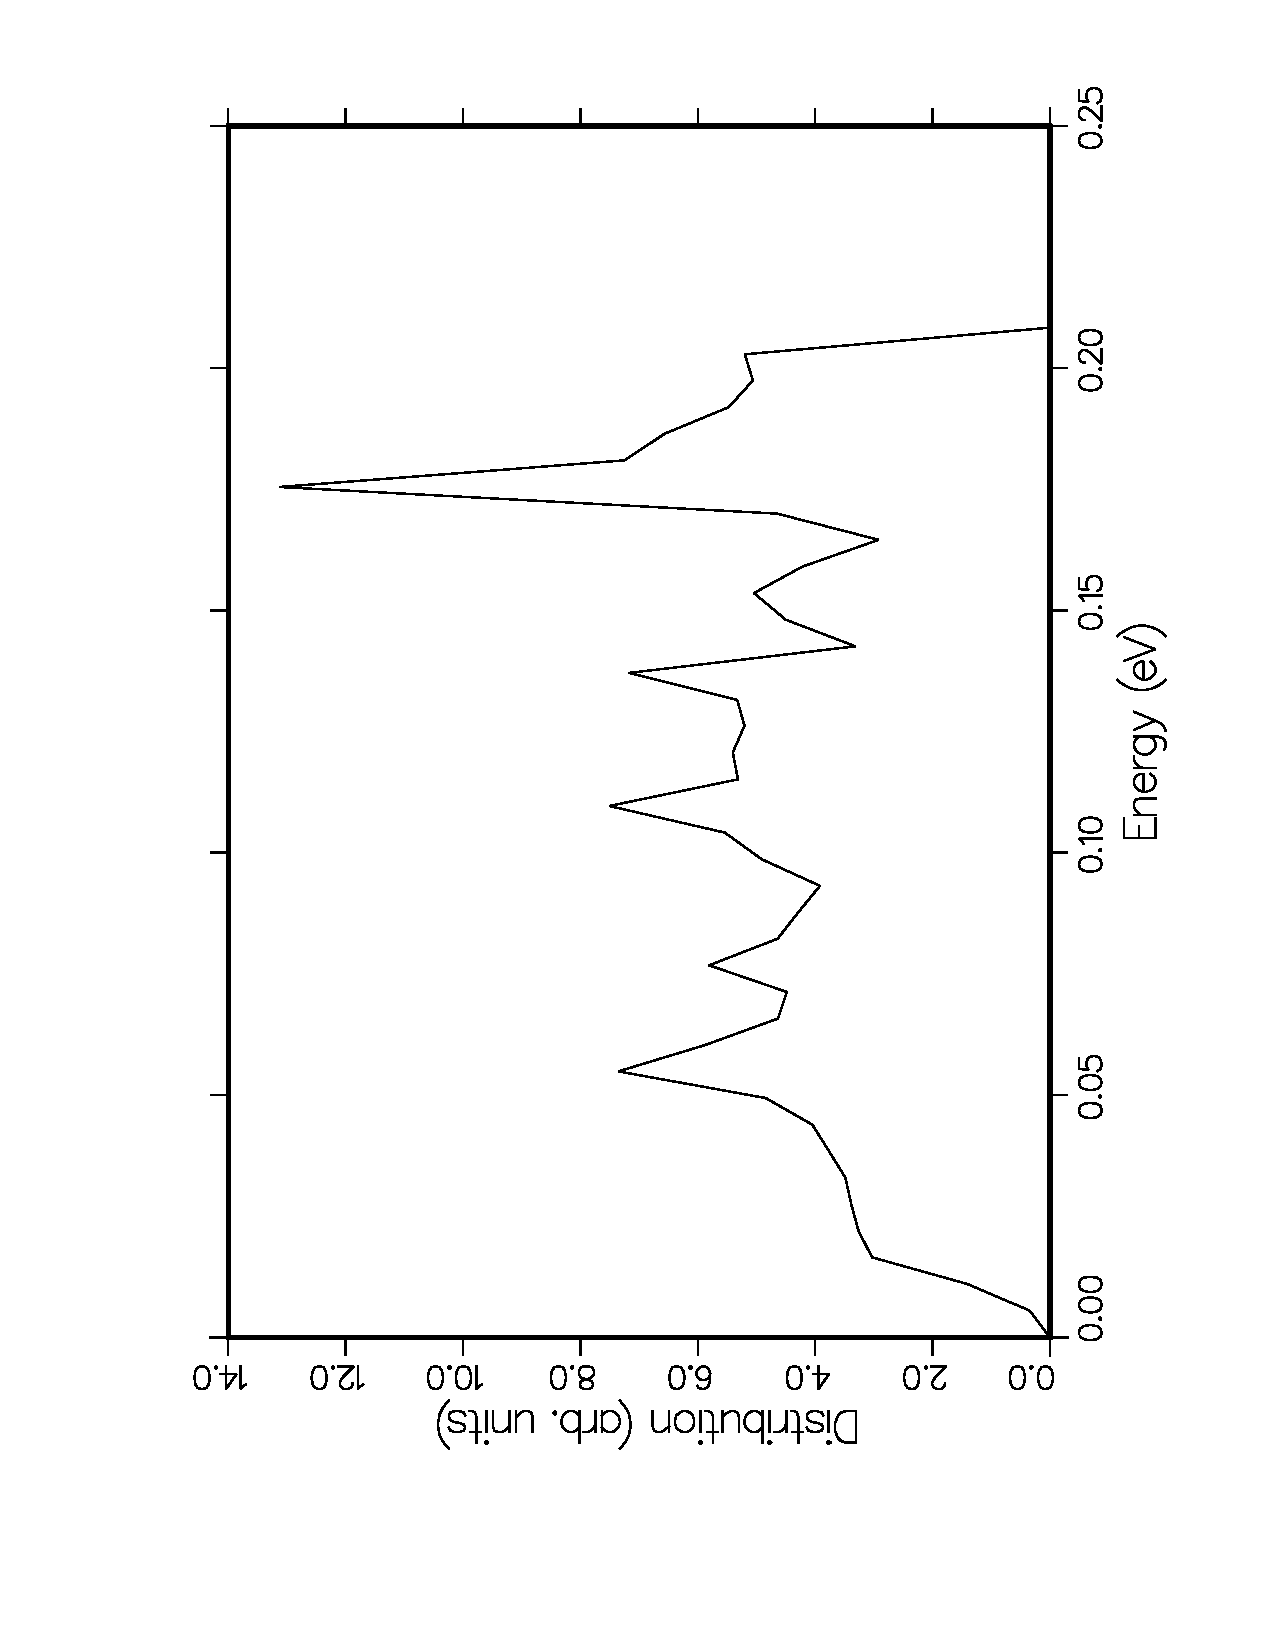
\includegraphics[keepaspectratio, height=3.7in, angle=270]{figs/leaack}
\caption[Graphite phonon frequency spectrum]{The phonon frequency
 spectrum $\rho(\epsilon)$ used for graphite.}
\label{graphr}
\end{figure}

\begin{figure}[b]\centering
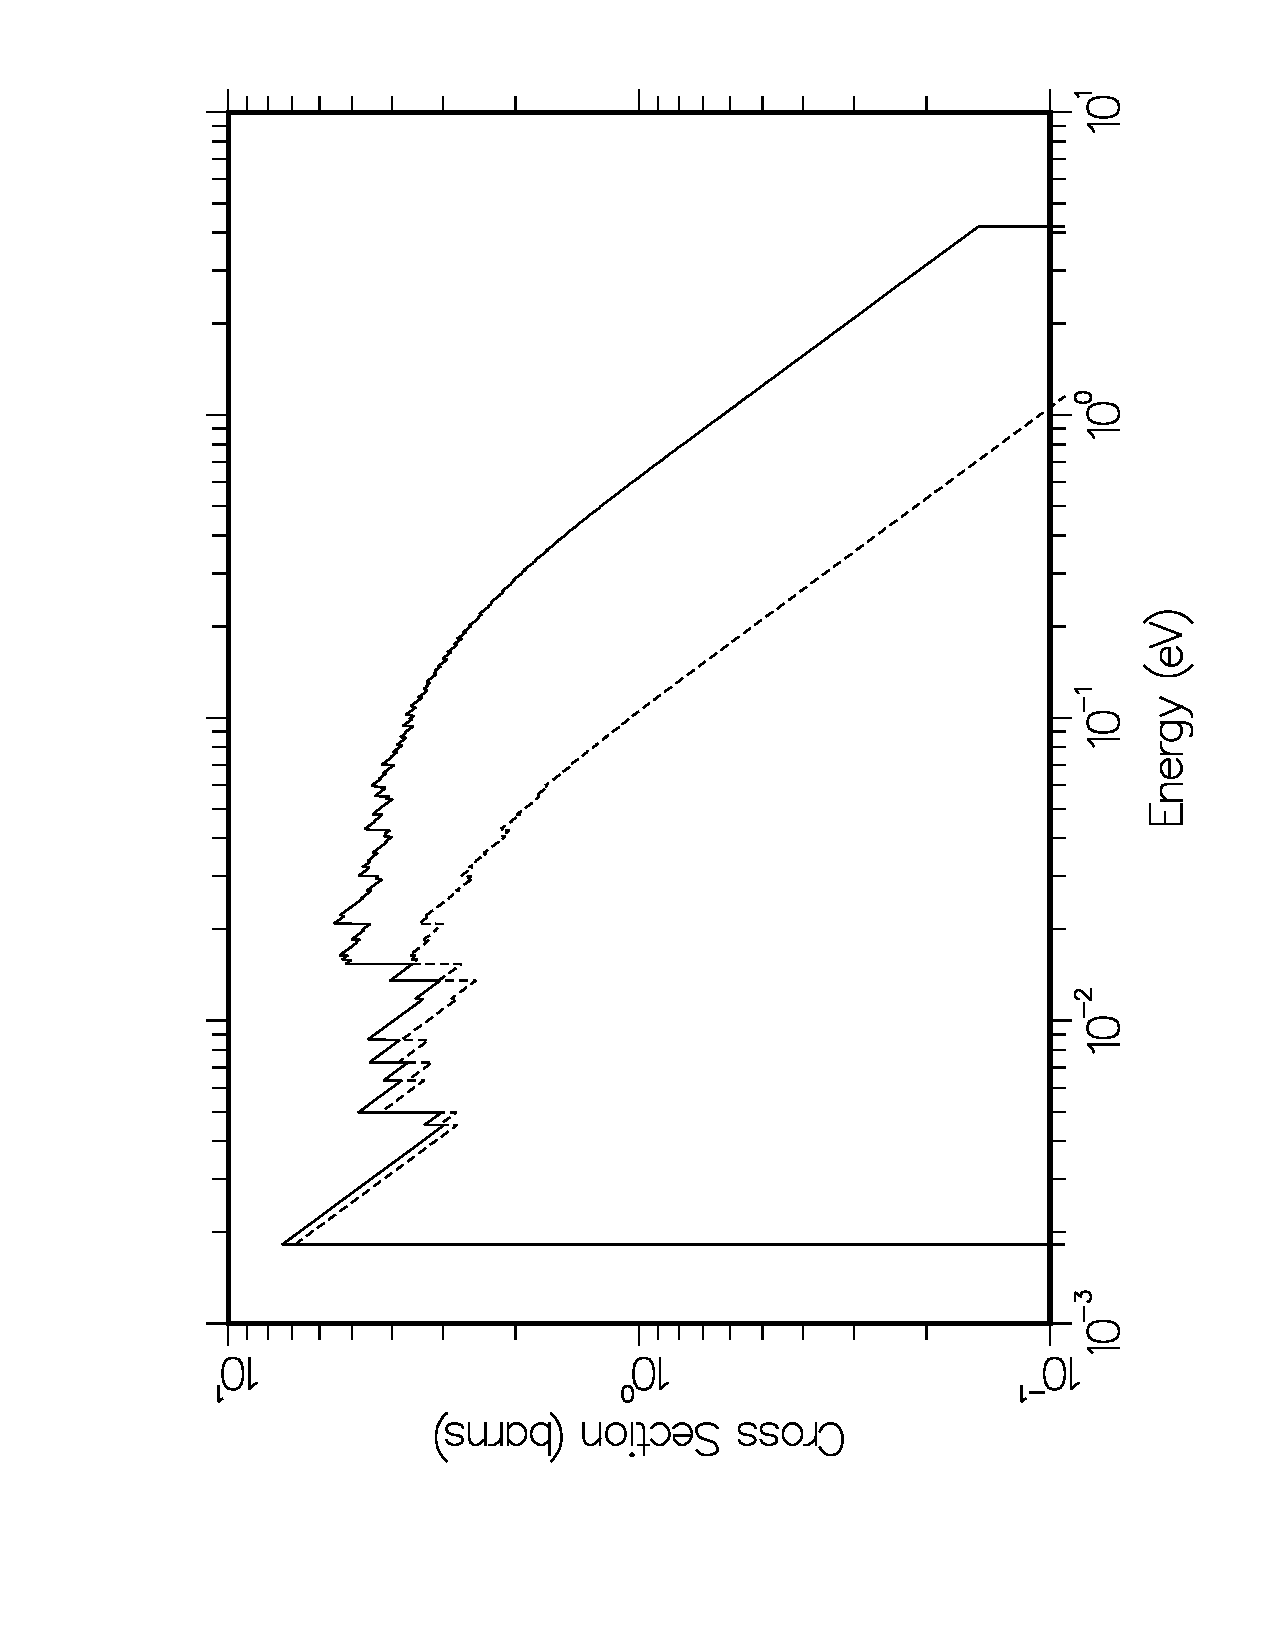
\includegraphics[keepaspectratio, height=3.7in, angle=270]{figs/leceack}
\caption[Coherent elastic scattering cross section for graphite]
{The coherent elastic cross section for graphite at temperatures of
 293.6K (solid) and 2000K (dashed) showing the Bragg peaks.  Note
 that the 293.6K cross section near the 4 eV breakpoint is still an
 appreciable part of the 4.74 barn free cross section.}
\label{gce}
\end{figure}

The rest of the sample input for graphite gives comment cards
to be entered into MF1/MT451 in the new evaluation.

After echoing back the input, the code prints out
$\rho(\beta)$, $P(\beta)$, and ${\cal T}_1(\beta)$ in normalized
form.  It then prints out the effective temperature for the SCT
approximation and the Debye-Waller factor needed for the coherent
scattering cross section calculation.  The break points between the
phonon expansion and the SCT are also shown.  LEAPR next computes the
$S(\alpha,\beta)$ function for each $\alpha$.  For quality control, it
displays the results of the normalization and sum rule tests.  If these
tests are not fairly close to unity, it may be necessary to tighten up
the grids used for the calculation.  Don't worry about test failures at
high values of $\alpha$; the $\beta$ grid will not extend to high enough
values to complete the integral over $\beta$.

An examination of the ENDF-6 output on ``tape20'' will show that both
coherent elastic scattering (MF=7/MT=2) and incoherent inelastic
scattering (MF=7/MT=4) are included in the new evaluation.  As shown
in Fig.~\ref{gce}, the the coherent scattering extends all the
way to 4 eV, which is an improvement over the original GA evaluation.
There is also enough range in $\alpha$ and $\beta$ grids to compute
thermal inelastic cross sections up to 4 eV.  See Fig.~\ref{gii}.

\begin{figure}[t]\centering
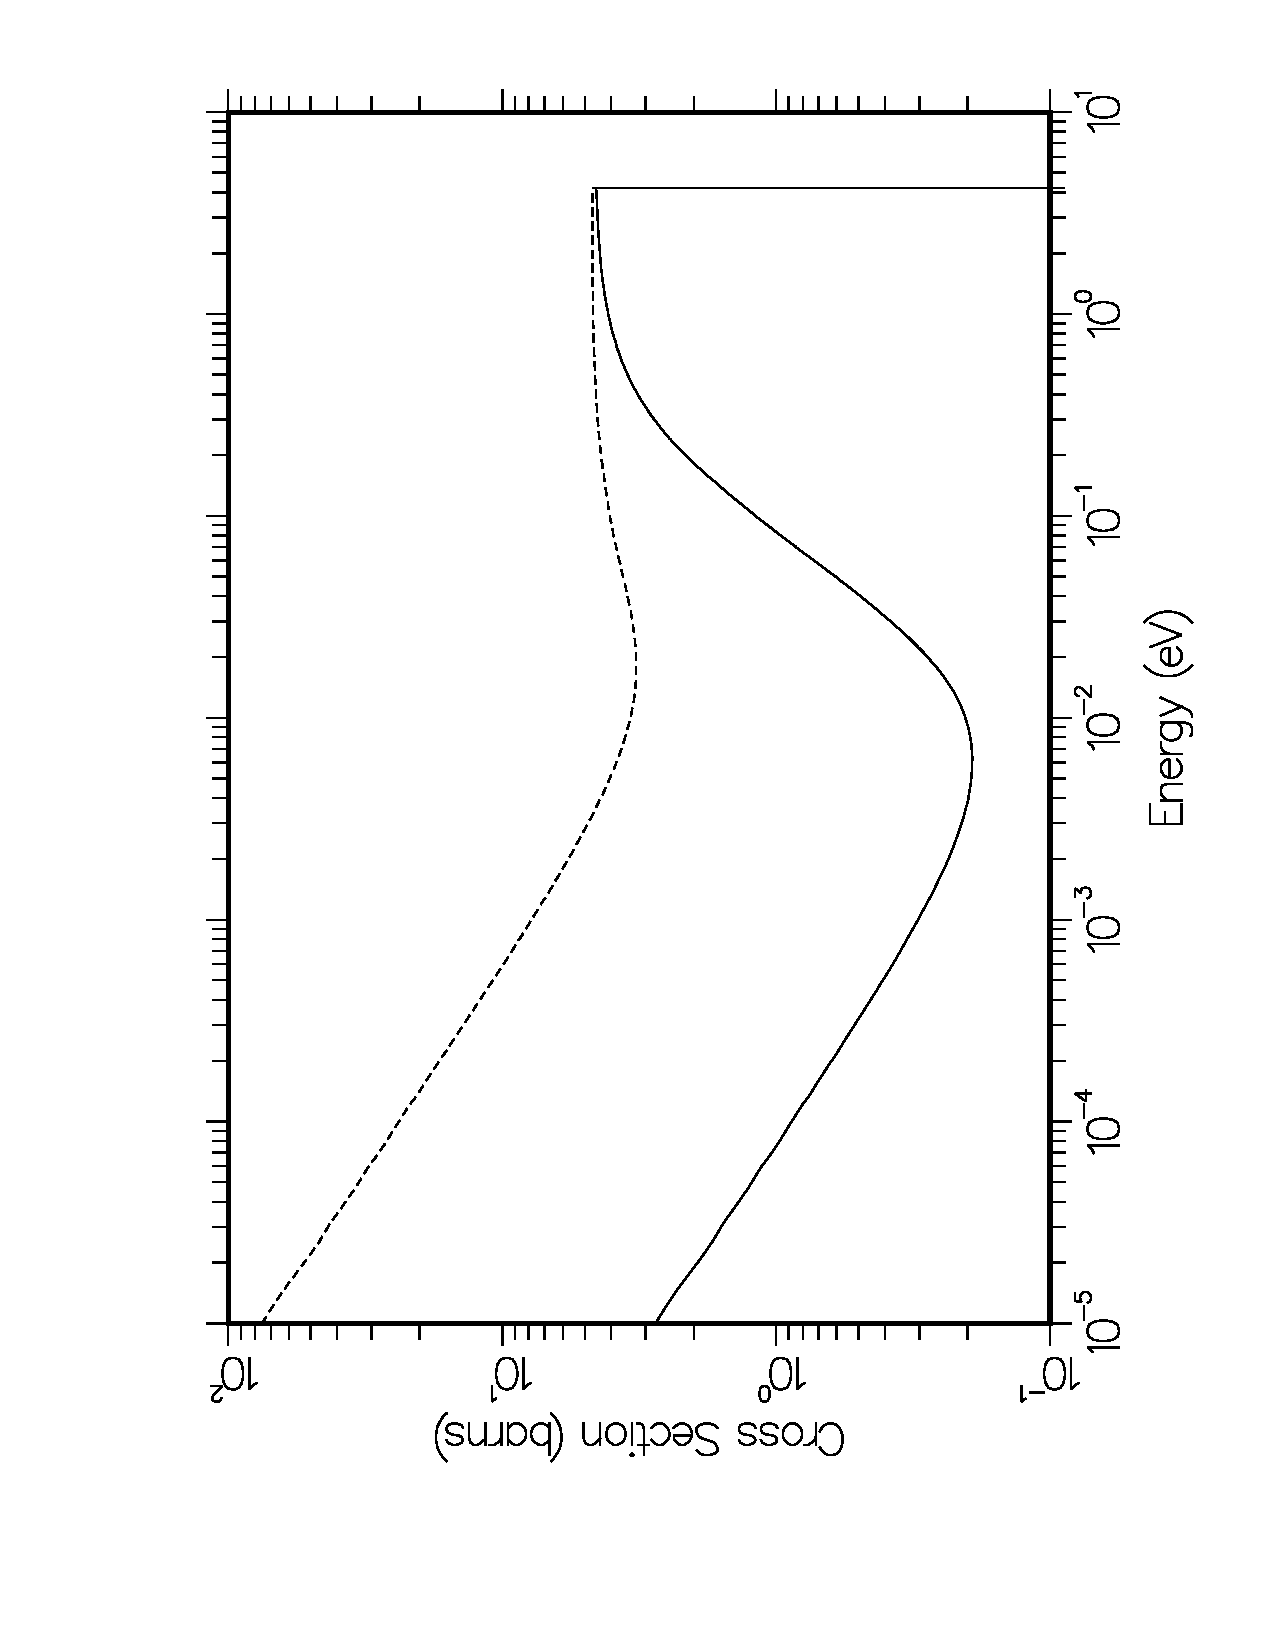
\includegraphics[keepaspectratio, height=3.7in, angle=270]{figs/leiiack}
\caption[Incoherent elastic scattering cross section for graphite]{The
 incoherent inelastic cross section for graphite at temperatures of
 293.6K (solid) and 2000K (dashed).  A comparison of the two curves
 near the 4 eV breakpoint shows that the 293.6K cross section still has
 not reached the 4.74 barn free cross section.  However, the sum of the
 elastic and inelastic components does equal the free value.}
\label{gii}
\end{figure}

\paragraph{The Model for BeO}\index{BeO}\index{mixed moderators}
This example demonstrates how to prepare a mixed $S(\alpha,\beta)$.
Actually, the evaluation used in ENDF/B-VII.0\index{ENDF!ENDF/B-VII} (and
later) splits the BeO case into separate parts for Be in BeO and O in BeO.
This earlier example is kept here to demonstrate the methods used
for preparing mixed moderators.

The basic physics was left unchanged from the GA evaluation
of 1969\cite{GAreport}.  Note that the following input deck contains both
``Be in BeO" and ``O in BeO".  The mixing option is selected by
the ``0." in the second field of input card 6.

\newpage
\small
\begin{ccode}

leapr
20/
'test of BeO in LEAPR'/
1/
27 4009/
8.93478 6.15 1 3/
1 0. 15.858 3.7481 1/
50 80 1/
.252 .504 .756 1.008 1.260 1.512 1.764 2.016 2.268 2.520 2.772 3.024
3.282 3.544 3.813 4.087 4.366 4.652 4.943 5.241 5.545 5.855 6.172 6.495
6.825 7.162 7.507 7.858 8.217 8.583 8.957 9.339 9.729 10.13 10.53 10.95
11.37 11.81 12.25 12.69 13.16 13.63 14.11 14.60 15.10 15.61 16.13 16.66
17.21 17.76/
0. .1513 .3025 .4537 .6049 .7561 .9073 1.059 1.210 1.361 1.512 1.663
1.815 1.966 2.117 2.268 2.419 2.571 2.722 2.873 3.024 3.176 3.327 3.478
3.629 3.780 3.932 4.083 4.241 4.408 4.583 4.766 4.958 5.159 5.371 5.592
5.825 6.069 6.325 6.593 6.875 7.170 7.480 7.805 8.146 8.504 8.879 9.273
9.686 10.12 10.57 11.05 11.55 12.07 12.62 13.20 13.81 14.44 15.11 15.81
16.54 17.31 18.12 18.96 19.85 20.78 21.76 22.78 23.86 24.99 26.17 27.41
28.71 30.08 31.51 33.01 34.59 36.24 37.98 39.80/
296/ Be in BeO
.0016518 84/
0.0 .3 .7 .9 1. 1.2 1.6 2.0 2.2 3.0 3.5 4.5 5.5 6.8 8.0 9.2 10.9 12.9
15.5 18.6 22.0 26.0 30.5 35.0 39.0 40.0 34.0 28.0 26.0 24.4 23.0
21.3 19.8 17.0 14.1 12.0 10.0 9.0 9.0 8.5 7.5 6.0 4.6 3.1 1.6
0.5 0. 0.0 4.0 15.0 38.0 52.0 70.0 105.0 165.0 230.0 200.0 170.0
145.0 136.0 134.0 112.0 96.0 89.0 84.0 75.0 87.0 81.0 66.0 59.0
68.0 105.0 95.0 97.0 135.0 163.0 130.0 111.0 92.0 67.0 45.0 19.0
7.0 0.0/
0. 0. 1./
0/
296/ O in BeO
.0016518 84/
0.0 0.4 0.8 1.0 1.4 2.0 2.5 3.5 4.8 6.2 8.9 11.0 14.0 17.2 21.5 26.5
34.0 40.0 46.0 58.0 60.0 93.0 110.0 129.0 141.0 142.0 125.0 101.0
93.0 92.0 91.0 95.0 95.0 98.0 108.0 93.0 78.0 98.0 112.0 115.0 145.0
160.0 190.0 190.0 120.0 43.0 0.0 0.0 1.0 9.0 19.0 26.0 35.0 48.0 66.0
92.0 82.0 56.0 44.0 35.0 29.0 21.0 15.0 11.5 9.0 8.0 7.0 6.0 5.2
4.5 5.0 5.9 6.0 5.0 4.0 2.5 1.8 1.0 0.50 0.50 0.20 0.0 0.0 0.0/
0. 0. 1. 0./
0/
'TEST COMMENTS'/
'FOR MF1/MT451 OF BEO'/
/
STOP

\end{ccode}
\normalsize

The output listing for this case starts with the output for the primary
scatterer ``Be in BeO" and continues with results for the secondary
scatterer ``O in BeO".  Note that the $\alpha$ values for the secondary
scatterer have been transformed by the atomic weight ratio of the two
atoms.  This allows us to add the $S(\alpha,\beta)$ contribution for
$\alpha_i$ from Be in BeO to the contribution for $\alpha_i$ from
O in BeO with only a cross-section weighting.  The resulting
$S(\alpha,\beta)$ is intended to be used with the beryllium cross sections.
The two frequency distributions are shown in Fig.~\ref{beo}.

\begin{figure}[b]\centering
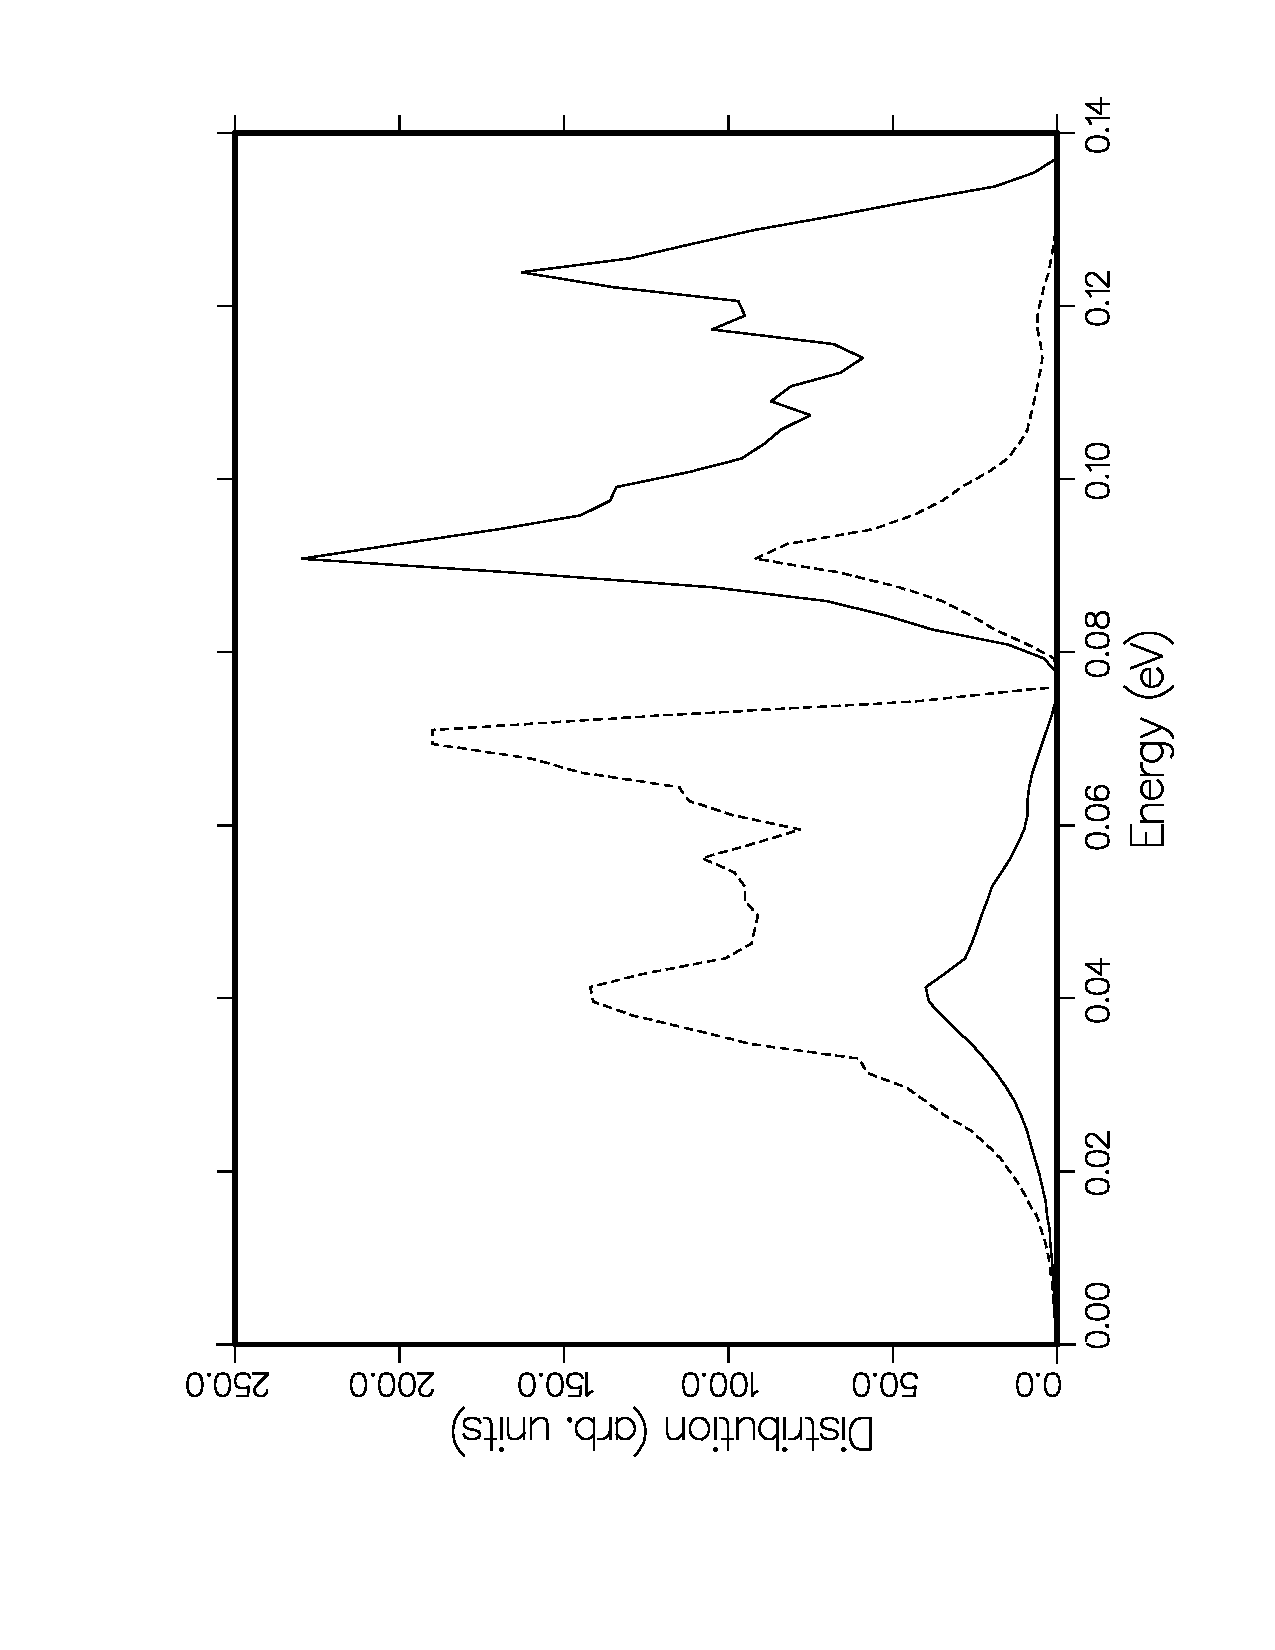
\includegraphics[keepaspectratio, height=3.7in, angle=270]{figs/leback}
\caption[Frequency spectra for BeO]{The frequency spectr
 $\rho(\epsilon)$ used for Be in BeO (solid) and O in BeO (dashed).}
\label{beo}
\end{figure}

The listing includes effective temperatures and Debye-Waller factors
for both constituents.  The average of the Debye-Waller factors is used
in computing the coherent elastic scattering for BeO.

The ENDF output on \cword{tape20} looks pretty much like the results for
graphite, except data for two scatterers is given at the start of MF=7/MT=4,
and two effective temperatures are given at the end of the section.

\begin{figure}[t]\centering
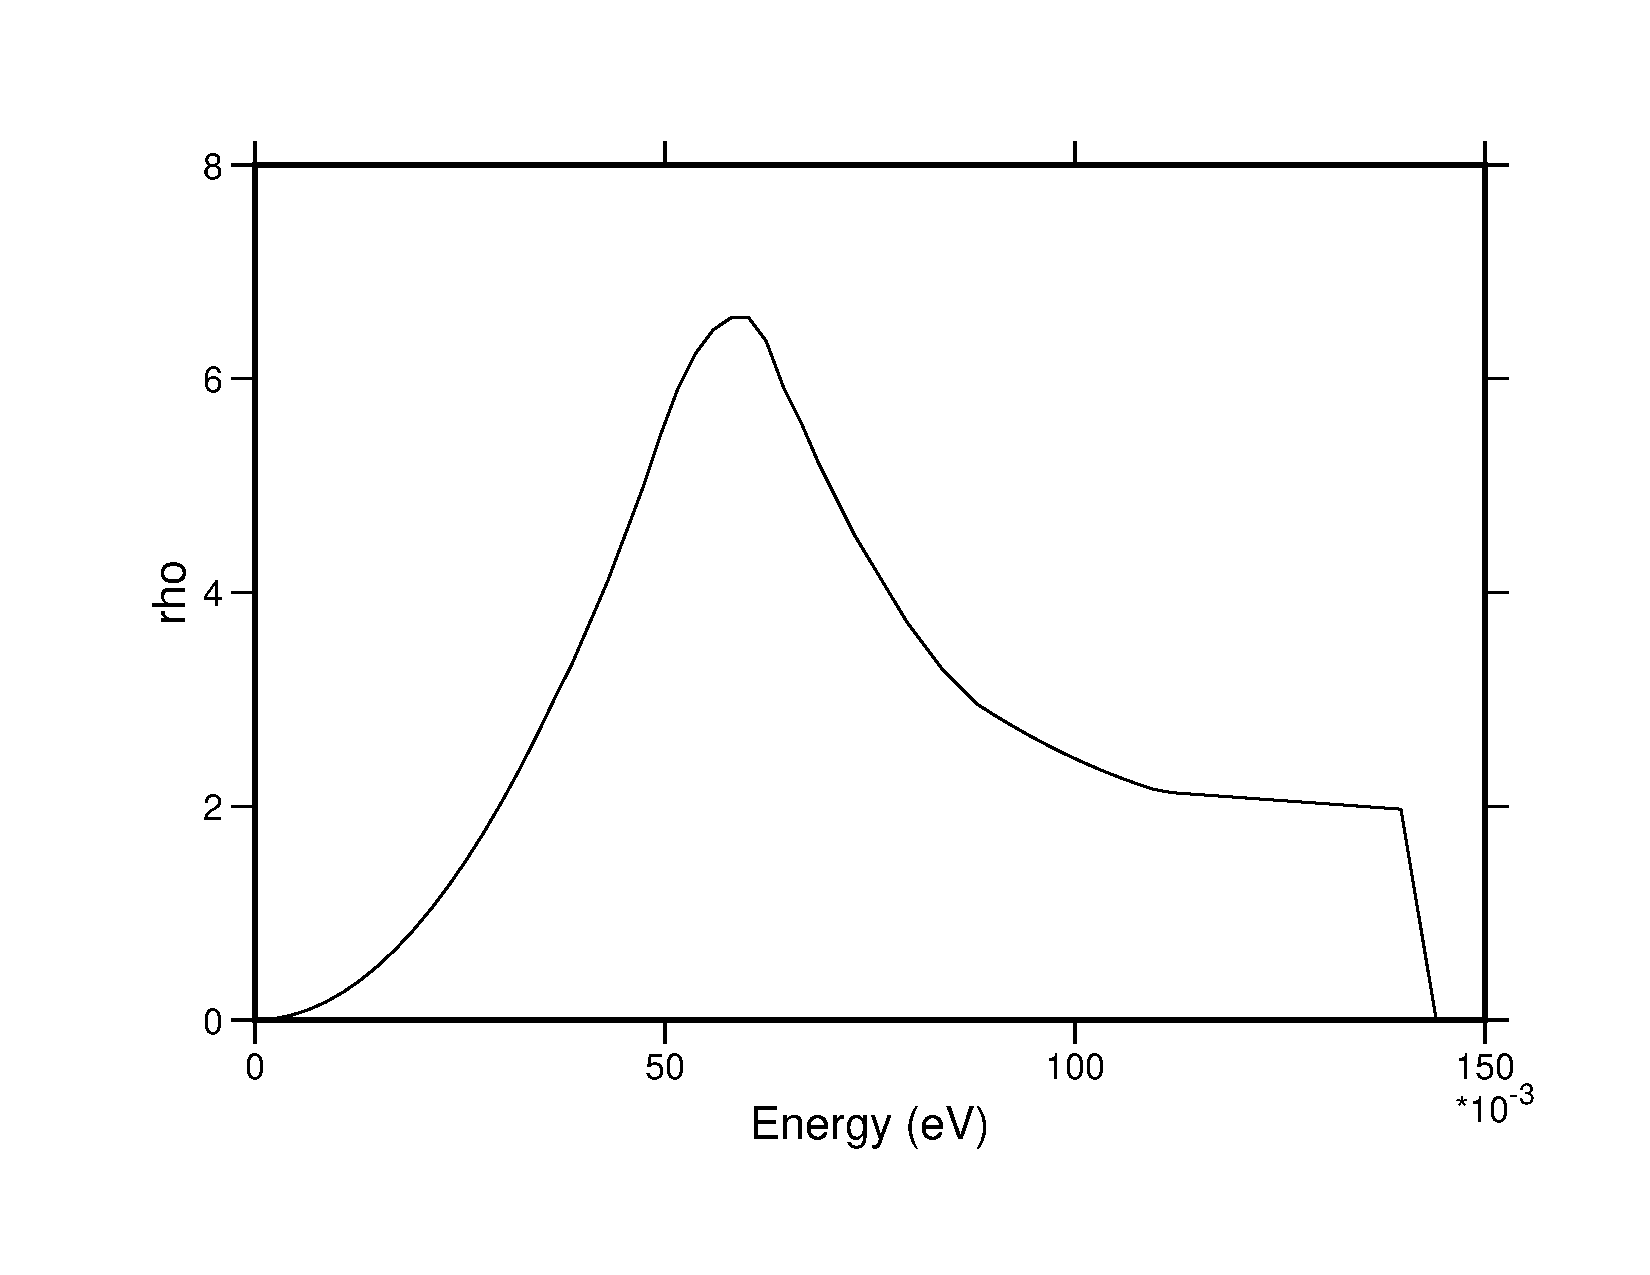
\includegraphics[keepaspectratio, height=3.7in, angle=0]{figs/hh2o-rhoack}
\caption[The frequency spectrum for H in H$_2$2O]{The frequency spectrum
 used for H in H$_2$O for ENDF/B-VII.0.}
\label{hh2o-rho}
\end{figure}

\paragraph{The Model for Water.}\index{water}
The current ENDF/B-VII.0 evaluation for the thermal scattering law for
H bound in H$_2$O is based on recent work done under IAEA\index{IAEA}
auspices\cite{mattes}\index{Mattes} with some slight modifications.
Mainly, the $\alpha$ and $\beta$ grids were extended and enhanced.  The
temperature grid was modified to be more like the other ENDF/B cases
by interpolating in the original distributions.  Note that the
frequency spectrum is temperature dependent in this input.  The 296K
spectrum is shown in Fig.~\ref{hh2o-rho}.  In
addition, the energy scale of the rotational spectrum was adjusted
slightly to improve agreement with experiment in the region
between 0.01 eV and 0.1 eV.  The final input deck is listed below.

\small
\begin{ccode}

leapr
20'
 ' H in H2O, IKE model modified at LANL'  /
 9 2 200/
 1 1001/
 0.99917 20.43634 2/  latest Hale values for VII
 1 1 1.585751+1 3.842443 1/   oxygen as free gas from VII
 187 274 1/  lat=1
     .001 .0015 .0025 .0035 .005 .007 .01 .015  .025 .035   .05  .070
     .1          .125      .15       .2        .25       .3        .325
     .35         .375      .4        .425      .45       .475      .5
     .525        .55       .58       .61       .65       .69       .73
     .78         .83       .88       .94       1.       1.08      1.16
    1.24        1.33      1.43      1.54       1.66     1.79      1.94
    2.09        2.26      2.48      2.7127     2.89     3.11      3.38
    3.67        3.98      4.32      4.65       5.0      5.4255    6.
    6.56        7.13      7.6       8.1026     8.8      9.5      10.2
   10.8152     11.7      12.6      13.528     14.4     15.3      16.2051
   17.233      18.2      18.92     20.3      21.63     22.9      24.308
   25.6        27.02     28.4      29.73     31.       32.41     33.44
   34.466      36.15     37.18     38.8      40.513    41.54     42.57
   44.2        46.0      47.0      48.615    49.6      51.2      52.5
   54.41       55.2      56.72     58.4      59.80     61.2      62.51
   63.8        65.23     66.5      67.90     68.93     70.61     71.64
   72.92       75.9      80.       84.       89.       94.      100.
  105.        113.      120.63    126.      132.      140.      147.
  154.        162.      170.      177.      184.      191.      199.
  208.        218.      227.      237.      246.      255.      265.
  275.72      284.      293.58    302.      311.      320.      329.
  338.        347.      356.      365.      374.      383.      392.
  401.        410.      419.      428.      437.      446.      455.
  464.        473.      482.      491.      500.      509.      518.
  527.        536.      545.      554.      563.      572.      581.
  590.        597.      604.      611.      618.      625.      632.9 / alpha
    0.0  0.005  0.01  0.015  0.020  0.025  0.030  0.040  0.050
    0.06  0.07  0.08 0.1  0.125
    0.15  0.175  0.20  0.225  0.250     0.30      0.35      0.40      0.45
    0.50        0.55      0.60      0.65      0.70      0.75      0.80
    0.85        0.90      0.95      1.0       1.05      1.10      1.15
    1.20        1.25      1.30      1.35      1.4       1.45      1.5
    1.55        1.6       1.65      1.7       1.75      1.8       1.85
    1.9         1.95      2.0       2.05      2.1       2.15      2.2
    2.25        2.3       2.35      2.4       2.45      2.5       2.55
    2.6         2.65     2.7127     2.77      2.83      2.90      2.96
    3.03        3.11      3.18      3.26      3.34      3.43      3.52
    3.61        3.71      3.81      3.92      4.03      4.14      4.26
    4.39        4.52      4.65      4.80      4.94      5.10      5.26
    5.4255      5.60      5.70      5.97      6.17      6.37      6.59
    6.81        7.04      7.29    7.54  7.81  7.9  8.0  8.103  8.2 8.28  8.37
    8.67        8.98      9.30      9.64     10.      10.4       10.8152
   11.16       11.57     12.0      12.46     12.98    13.528     13.94
   14.48       15.03     15.62     16.2051   16.8 17.  17.233  17.5  18.2
   18.92       19.4      19.95     20.7     21.63     22.1       22.66
   23.5        24.308    24.8      25.34    26.2      27.02      27.5
   28.05       28.9      29.73     30.2     30.76     31.5       32.41
   32.9        33.44     34.       34.466    35.3     36.15      36.6
   37.18       37.9      38.8      39.89     40.2     40.513     41.
   41.54       42.       42.57     43.2      44.2     45.28      46.0
   47.0        47.99     48.3      48.615    49.6     50.67      51.2
   51.70       52.5      53.38     53.9      54.41    55.2       56.
   56.72       57.12     58.4      59.80     61.2     62.51      63.8
   65.23       66.5      67.90     68.4      68.93    69.8       70.61
   71.1        71.64     72.2      72.92     73.3340  74.        74.8
   75.6        76.4      77.2      78.       78.9     79.8       80.7
   81.6        82.5      83.4      84.3      85.2     86.1       87.
   88.         89.       90.       91.       92.      93.        94.
   95.         96.       97.       98.       99.     100.       101.2
  102.4       103.6     104.8     106.      107.2    108.4      109.6
  110.8       112.      113.5     115.      116.5    118.       119.5
  121.        122.5     124.      125.5     127.     128.5      130.
  132.        134.      136.      138.      140.     142.       144.
  146.        148.      150.      152.      154.     156.       158.1 /  beta
 293.6/  temperature (K)
 0.00215 68/  frequency distribution
  0.00000E+00  1.04170E-02  4.16710E-02  9.37490E-02  1.66682E-01
  2.60457E-01  3.74972E-01  5.10341E-01  6.66586E-01  8.43707E-01
  1.04169E+00  1.26039E+00  1.49991E+00  1.76047E+00  2.04172E+00
  2.34379E+00  2.66665E+00  3.01045E+00  3.33873E+00  3.72164E+00
  4.10441E+00  4.54222E+00  4.98019E+00  5.47328E+00  5.91196E+00
  6.24071E+00  6.45971E+00  6.56965E+00  6.56980E+00  6.35010E+00
  5.91059E+00  5.58143E+00  5.19738E+00  4.86852E+00  4.53952E+00
  4.26544E+00  3.99124E+00  3.71714E+00  3.49814E+00  3.27889E+00
  3.11484E+00  2.95067E+00  2.84650E+00  2.74784E+00  2.65469E+00
  2.56706E+00  2.48495E+00  2.40835E+00  2.33727E+00  2.27169E+00
  2.21165E+00  2.15711E+00  2.12732E+00  2.11543E+00  2.10353E+00
  2.09165E+00  2.07975E+00  2.06786E+00  2.05596E+00  2.04408E+00
  2.03218E+00  2.02029E+00  2.00839E+00  1.99651E+00  1.98461E+00
  1.97272E+00  9.86360E-01  0.00000E+00/
    0.0192  0.  .4904 /      weights
    2 /                      discrete oscillators
   .205  .436 /              oscillator energies (eV)
    .163467   .326933  /     oscillator weigths
 350./
 0.00215 68/
 0.00215 68/
  0.00000E+00  1.01473E-02  4.05927E-02  9.13258E-02  1.62372E-01
  2.53717E-01  3.65283E-01  4.97147E-01  6.49350E-01  8.21883E-01
  1.01473E+00  1.22779E+00  1.46112E+00  1.71490E+00  1.98888E+00
  2.28315E+00  2.59770E+00  2.93259E+00  3.25984E+00  3.63884E+00
  4.02767E+00  4.45671E+00  4.88387E+00  5.34035E+00  5.73991E+00
  6.04488E+00  6.25544E+00  6.34641E+00  6.34077E+00  6.15681E+00
  5.79298E+00  5.49979E+00  5.16054E+00  4.85982E+00  4.56082E+00
  4.31061E+00  4.06087E+00  3.81176E+00  3.60561E+00  3.39981E+00
  3.23731E+00  3.06474E+00  2.95935E+00  2.84908E+00  2.74389E+00
  2.64100E+00  2.54595E+00  2.45437E+00  2.37253E+00  2.29361E+00
  2.22288E+00  2.15259E+00  2.10362E+00  2.07303E+00  2.04091E+00
  2.00986E+00  1.98036E+00  1.95997E+00  1.93780E+00  1.91648E+00
  1.89595E+00  1.87631E+00  1.86017E+00  1.84223E+00  1.82513E+00
  1.80884E+00  8.99437E-01  0.00000E+00/
    0.029135  0.  .485433 /
    2 /
   .205  .436 /
    .161811   .323622 /
 400/
 0.00215 68/
  0.00000E+00  9.92998E-03  3.97244E-02  8.93749E-02  1.58902E-01
  2.48290E-01  3.57482E-01  4.86523E-01  6.35474E-01  8.04310E-01
  9.93028E-01  1.20154E+00  1.42988E+00  1.67821E+00  1.94634E+00
  2.23432E+00  2.54218E+00  2.86990E+00  3.19677E+00  3.57300E+00
  3.96771E+00  4.38985E+00  4.80833E+00  5.23385E+00  5.60019E+00
  5.88507E+00  6.08865E+00  6.16336E+00  6.15269E+00  5.99938E+00
  5.70048E+00  5.43794E+00  5.13693E+00  4.86008E+00  4.58656E+00
  4.35661E+00  4.12764E+00  3.89978E+00  3.70442E+00  3.50993E+00
  3.34851E+00  3.16838E+00  3.06178E+00  2.94128E+00  2.82550E+00
  2.70924E+00  2.60283E+00  2.49814E+00  2.40685E+00  2.31627E+00
  2.23617E+00  2.15212E+00  2.08649E+00  2.03966E+00  1.98998E+00
  1.94228E+00  1.89751E+00  1.86973E+00  1.83863E+00  1.80911E+00
  1.78107E+00  1.75470E+00  1.73486E+00  1.71165E+00  1.69001E+00
  1.66990E+00  8.25640E-01  0.00000E+00/
    0.0346475  0.  .482676 /
    2 /
   .205  .436  /
   0.160892    0.321784 /
 450/
 0.00215 68/
  0.00000E+00  9.75410E-03  3.90199E-02  8.77925E-02  1.56087E-01
  2.43887E-01  3.51155E-01  4.77906E-01  6.24218E-01  7.90054E-01
  9.75417E-01  1.18024E+00  1.40455E+00  1.64845E+00  1.91182E+00
  2.19470E+00  2.49715E+00  2.81904E+00  3.14676E+00  3.52166E+00
  3.92356E+00  4.34050E+00  4.75201E+00  5.14878E+00  5.48392E+00
  5.75016E+00  5.94766E+00  6.00672E+00  5.99108E+00  5.86722E+00
  5.63083E+00  5.39736E+00  5.13269E+00  4.87821E+00  4.62866E+00
  4.41770E+00  4.20824E+00  4.00034E+00  3.81484E+00  3.63071E+00
  3.46976E+00  3.28157E+00  3.17338E+00  3.04241E+00  2.91583E+00
  2.78605E+00  2.66813E+00  2.55020E+00  2.44932E+00  2.34697E+00
  2.25742E+00  2.15958E+00  2.07737E+00  2.01447E+00  1.94741E+00
  1.88323E+00  1.82333E+00  1.78821E+00  1.74824E+00  1.71058E+00
  1.67508E+00  1.64202E+00  1.61848E+00  1.59002E+00  1.56386E+00
  1.53993E+00  7.56386E-01  0.00000E+00/
    0.0385185  0.  .480741 /
    2 /
   .205  .436 /
    0.160247   0.320494 /
 500./
 0.00215 68/
  0.00000E+00  9.59182E-03  3.83708E-02  8.63356E-02  1.53495E-01
  2.39833E-01  3.45330E-01  4.69972E-01  6.13855E-01  7.76930E-01
  9.59202E-01  1.16064E+00  1.38122E+00  1.62104E+00  1.88004E+00
  2.15823E+00  2.45569E+00  2.77222E+00  3.10113E+00  3.47514E+00
  3.88458E+00  4.29687E+00  4.70201E+00  5.07095E+00  5.37579E+00
  5.62401E+00  5.81575E+00  5.85948E+00  5.83894E+00  5.74390E+00
  5.56870E+00  5.36355E+00  5.13433E+00  4.90155E+00  4.67527E+00
  4.48277E+00  4.29224E+00  4.10374E+00  3.92773E+00  3.75358E+00
  3.59291E+00  3.39657E+00  3.28670E+00  3.14529E+00  3.00795E+00
  2.86472E+00  2.73536E+00  2.60427E+00  2.49386E+00  2.37982E+00
  2.28086E+00  2.16936E+00  2.07076E+00  1.99198E+00  1.90775E+00
  1.82730E+00  1.75245E+00  1.71007E+00  1.66134E+00  1.61563E+00
  1.57276E+00  1.53308E+00  1.50587E+00  1.47223E+00  1.44158E+00
  1.41387E+00  6.89143E-01  0.00000E+00/
    0.0417390  0.      0.479131    /
    2 /
   .205  .436 /
    .159710  .319420 /
 550./
 0.00215 68/
  0.00000E+00  9.44225E-03  3.77730E-02  8.49922E-02  1.51106E-01
  2.36096E-01  3.39961E-01  4.62659E-01  6.04301E-01  7.64830E-01
  9.44252E-01  1.14257E+00  1.35972E+00  1.59577E+00  1.85074E+00
  2.12460E+00  2.41747E+00  2.72905E+00  3.05951E+00  3.43307E+00
  3.85041E+00  4.25857E+00  4.65785E+00  4.99971E+00  5.27495E+00
  5.50565E+00  5.69192E+00  5.72054E+00  5.69514E+00  5.62848E+00
  5.51353E+00  5.33613E+00  5.14167E+00  4.93008E+00  4.72654E+00
  4.55204E+00  4.38002E+00  4.21047E+00  4.04363E+00  3.87915E+00
  3.71857E+00  3.51397E+00  3.40232E+00  3.25044E+00  3.10232E+00
  2.94564E+00  2.80482E+00  2.66059E+00  2.54064E+00  2.41493E+00
  2.30656E+00  2.18144E+00  2.06653E+00  1.97198E+00  1.87070E+00
  1.77407E+00  1.68437E+00  1.63478E+00  1.57734E+00  1.52363E+00
  1.47343E+00  1.42716E+00  1.39631E+00  1.35749E+00  1.32239E+00
  1.29091E+00  6.23480E-01  0.00000E+00/
    0.044466  0.      0.477767  /
    2 /
   .205  .436 /
   0.159256   0.318512 /
 600./
 0.00215 68/
  0.00000E+00  9.30614E-03  3.72301E-02  8.37725E-02  1.48936E-01
  2.32702E-01  3.35086E-01  4.56017E-01  5.95626E-01  7.53841E-01
  9.30674E-01  1.12615E+00  1.34019E+00  1.57282E+00  1.82412E+00
  2.09406E+00  2.38276E+00  2.68985E+00  3.02226E+00  3.39584E+00
  3.82152E+00  4.22611E+00  4.62011E+00  4.93565E+00  5.18198E+00
  5.39565E+00  5.57674E+00  5.59048E+00  5.56024E+00  5.52153E+00
  5.46600E+00  5.31580E+00  5.15545E+00  4.96453E+00  4.78321E+00
  4.62629E+00  4.47234E+00  4.32131E+00  4.16331E+00  4.00819E+00
  3.84750E+00  3.63447E+00  3.52091E+00  3.35849E+00  3.19952E+00
  3.02936E+00  2.87703E+00  2.71964E+00  2.59009E+00  2.45269E+00
  2.33489E+00  2.19614E+00  2.06498E+00  1.95472E+00  1.83644E+00
  1.72372E+00  1.61923E+00  1.56244E+00  1.49632E+00  1.43462E+00
  1.37712E+00  1.32429E+00  1.28978E+00  1.24581E+00  1.20626E+00
  1.17101E+00  5.59371E-01  0.00000E+00/
    0.046537  0.   0.476732  /
    2 /
   .205  .436  /
   0.158911        0.317821  /
 650./
 0.00215 68/
  0.00000E+00  9.20968E-03  3.68424E-02  8.29024E-02  1.47390E-01
  2.30283E-01  3.31608E-01  4.51281E-01  5.89440E-01  7.46008E-01
  9.20999E-01  1.11445E+00  1.32627E+00  1.55647E+00  1.80516E+00
  2.07229E+00  2.35801E+00  2.66190E+00  2.99405E+00  3.36630E+00
  3.79437E+00  4.19585E+00  4.58597E+00  4.88805E+00  5.11997E+00
  5.32491E+00  5.50293E+00  5.50965E+00  5.47725E+00  5.45177E+00
  5.42426E+00  5.28734E+00  5.14353E+00  4.96297E+00  4.79271E+00
  4.64457E+00  4.49963E+00  4.35781E+00  4.20453E+00  4.05433E+00
  3.89416E+00  3.67795E+00  3.56391E+00  3.39713E+00  3.23364E+00
  3.05777E+00  2.90060E+00  2.73760E+00  2.60402E+00  2.46163E+00
  2.33984E+00  2.19520E+00  2.05689E+00  1.93967E+00  1.81386E+00
  1.69399E+00  1.58295E+00  1.52299E+00  1.45304E+00  1.38783E+00
  1.32711E+00  1.27139E+00  1.23530E+00  1.18907E+00  1.14757E+00
  1.11069E+00  5.27354E-01  0.00000E+00/
    0.049020  0.     0.47549 /
    2 /
   .205  .436 /
   0.158497        0.316993  /
 800./
 0.00215 68/
  0.00000E+00  9.20968E-03  3.68424E-02  8.29024E-02  1.47390E-01
  2.30283E-01  3.31608E-01  4.51281E-01  5.89440E-01  7.46008E-01
  9.20999E-01  1.11445E+00  1.32627E+00  1.55647E+00  1.80516E+00
  2.07229E+00  2.35801E+00  2.66190E+00  2.99405E+00  3.36630E+00
  3.79437E+00  4.19585E+00  4.58597E+00  4.88805E+00  5.11997E+00
  5.32491E+00  5.50293E+00  5.50965E+00  5.47725E+00  5.45177E+00
  5.42426E+00  5.28734E+00  5.14353E+00  4.96297E+00  4.79271E+00
  4.64457E+00  4.49963E+00  4.35781E+00  4.20453E+00  4.05433E+00
  3.89416E+00  3.67795E+00  3.56391E+00  3.39713E+00  3.23364E+00
  3.05777E+00  2.90060E+00  2.73760E+00  2.60402E+00  2.46163E+00
  2.33984E+00  2.19520E+00  2.05689E+00  1.93967E+00  1.81386E+00
  1.69399E+00  1.58295E+00  1.52299E+00  1.45304E+00  1.38783E+00
  1.32711E+00  1.27139E+00  1.23530E+00  1.18907E+00  1.14757E+00
  1.11069E+00  5.27354E-01  0.00000E+00/
    0.049020  0.   0.47549 /
    2 /
   .205  .436 /
   0.158497        0.316993  /
  ' H(H2O)    IKE,LANL   EVAL-mar06 MacFarlane,Keinert,Mattes        '/
  ' INDC-NDS-0470        DIST-                                       '/
  '----ENDF/B-VII        MATERIAL    1                               '/
  '-----THERMAL NEUTRON SCATTERING DATA                              '/
  '------ENDF-6 FORMAT                                               '/
  '                                                                  '/
  ' Temperatures (K)                                                 '/
  '         293.6  350  400  450  500  550  600  650  800            '/
  '                                                                  '/
  ' This evaluation[1] was generated at IKE in January of 2004 using '/
  ' the LEAPR module of the NJOY Nuclear Data Processing System[2]   '/
  ' and modified at LANL in March of 2006 to use a temperature grid  '/
  ' more like the other ENDF evaluations and to fit the experimental '/
  ' data slightly better.  The model is improved over the one used   '/
  ' at General Atomics in 1969 to produce the original ENDF/B-III    '/
  ' evaluation[3].  The alpha and beta grids have been extended to   '/
  ' allow for larger incident energies and to properly represent the '/
  ' features of S(alpha,beta) for the various integrations required. '/
  ' The physical constants have been updated for ENDF/B-VII to match '/
  ' the current hydrogen and oxygen evaluations.  The LANL changes   '/
  ' include some additional alpha and beta points, interpolating the '/
  ' rotational energy distributions and translational masses onto    '/
  ' the new temperature grid, and slightly reducing the rotational   '/
  ' energies to improve the energy region between .01 and .1 eV.     '/
  '                                                                  '/
  ' Water is represented by freely moving H2O molecule clusters      '/
  ' with some temperature dependence to the clustering effect.       '/
  ' Each molecule can undergo torsional harmonic oscillations        '/
  ' (hindered rotations) with a broad spectrum of distributed        '/
  ' modes. The excitation spectra were improved over the older       '/
  ' ENDF model, and they are given with a temperature variation.     '/
  ' In addition, there are two internal modes of vibration at        '/
  ' 205 and 436 meV.  The stretching mode was reduced from the       '/
  ' older ENDF value of 480 meV to account for the liquid state.     '/
  ' Scattering by the oxygen atoms is not included in the            '/
  ' tabulated scattering law data.  It should be taken into          '/
  ' account by adding the scattering for free oxygen of mass 16.     '/
  '                                                                  '/
  ' References                                                       '/
  ' ----------                                                       '/
  ' 1. M.Mattes and J.Keinert, "Thermal Neutron Scattering Data      '/
  '    for the Moderator Materials H2O, D2O, and ZrHx in ENDF-6      '/
  '    Format and as ACE Library for MCNP(X) Codes," INDC/NDS        '/
  '    report INDC(NDS)-0470 (April 2005).                           '/
  ' 2. R.E.MacFarlane, "New Thermal Neutron Scattering Files for     '/
  '    ENDF/B-VI Release 2," Los Alamos National Laboratory report   '/
  '    LA-12639-MS (March 1994).                                     '/
  ' 3. J.U.Koppel and D.H.Houston, "Reference Manual for ENDF        '/
  '    Thermal Neutron Scattering Data," General Atomic report       '/
  '    GA-8774 revised and reissued as ENDF-269 by the National      '/
  '    Nuclear Data Center, July 1978.                               '/
  '                                                                  '/
  ' ---------------------------------------------------------------- '/
  /  end leapr
  stop

\end{ccode}
\normalsize

These $\alpha$ and $\beta$ grids extend to rather high values
in order to allow calculations of water cross sections to energies
on the order of 10 eV.

This run specifies \cword{iprint}=2 to get a more detailed output listing.
Note that the listing now includes checks for the normalization of the
phonon expansion members, ${\cal T}_n$.  It also prints out the values
$S(\alpha,\beta)$, ${\cal S}(\alpha,\beta)$, and ${\cal S}(\alpha,-\beta)$
for each $\beta$.  Note that only the asymmetric S for $-\beta$ is
actually used and stored inside the code.  The other two versions are
computed just before being printed.  On a short-word machine, these first
two styles of $S$ may underflow and be printed as zero, even though the
last column is nonzero.  No accuracy is actually lost at this point.

After the results for the solid-type rotational modes have been printed
out, the code starts a print for the convolution of the translational
modes with the continuous modes.  For each $\alpha$, the values for
$S_{\rm free}$ are printed out, followed by the results of the
convolution, and the results of the normalization and sum-rule tests.
These results can be examined to see if the $\beta$ grid seems to be
sufficient for the problem.  The problem here is that the translational
peak is very sharp for small $\alpha$, and it is difficult to make the
$\beta$ grid fine enough to represent it well.  Some loss in the
normalization and sum-rule accuracies must be accepted.

Next, the code shows similar results for the convolution of the discrete
oscillators\index{discrete oscillators} with the current scattering law.
Now the problem is that new peaks appear at the $n\beta_i$ values and
their various sums and differences (see Table~\ref{oscwts} for examples).
For small $\alpha$, these peaks are very sharp.  A few additional
$\beta$ points can be added near the peaks to improve the results, but
it is usually impractical to represent them with full fidelity.  Once
again, some loss in the accuracy of the checks must be accepted.

\begin{table}[ht]
\begin{center}
\caption[Oscillator beta values for $\alpha=1$ for H in H$_2$O]{Discrete
 oscillator $\beta$ values and weights for $\alpha=1$ for H in H$_2$O.}
\vspace{3mm}
\label{oscwts}
\hspace{-10mm}\begin{tabular}{rr}
\bf\small Beta & \bf\small Weight \\ \hline
0.0000 & 9.6160E-01 \\
-8.1026 & 1.9405E-02 \\
-17.2328 & 1.8243E-02 \\
-25.3353 & 3.6814E-04 \\
-16.2051 & 1.9580E-04 \\
-34.4655 & 1.7304E-04 \\
8.1026 & 5.8752E-06 \\
-33.4379 & 3.7146E-06 \\
-42.5680 & 4.4920E-06 \\
-24.3077 & 1.3171E-06 \\
-51.6983 & 1.0943E-06 \\ \hline
\end{tabular}
\end{center}
\end{table}

\begin{figure}[b]\centering
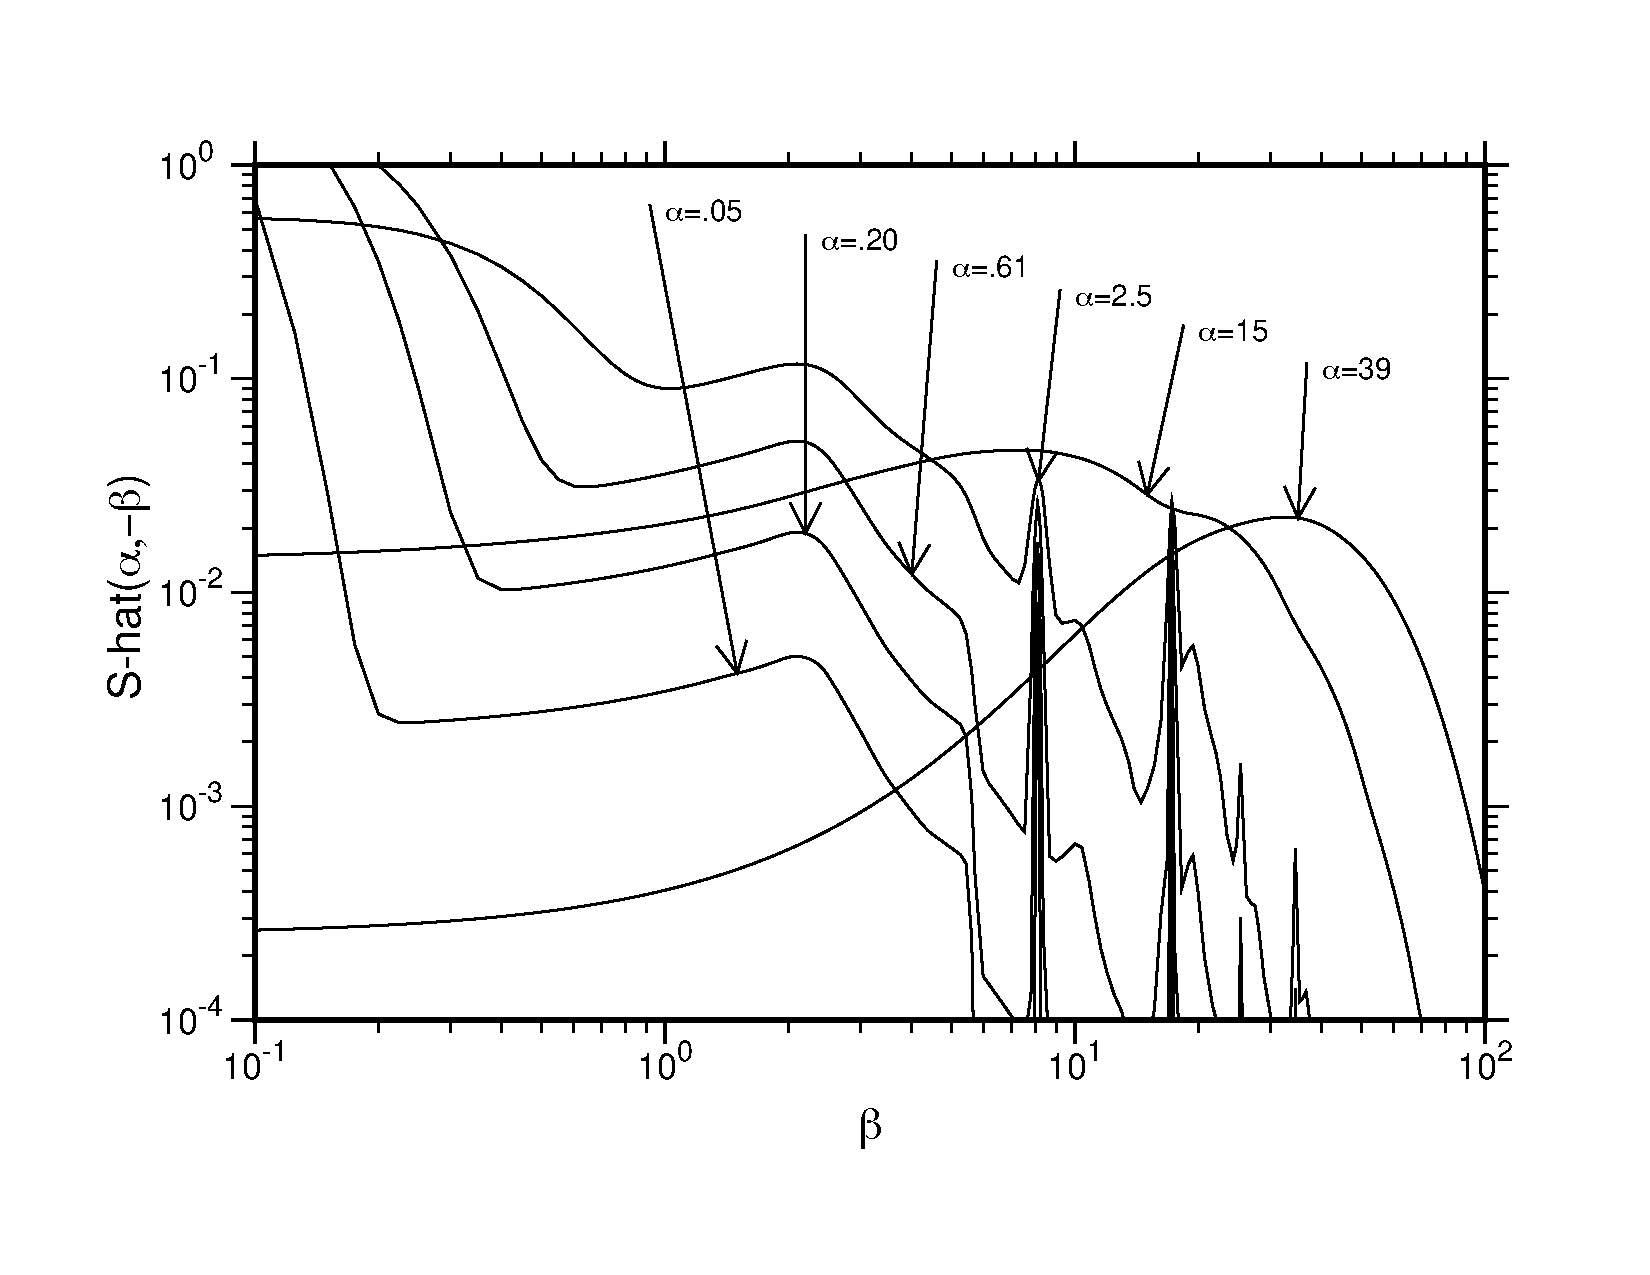
\includegraphics[keepaspectratio, height=3.5in, angle=0]{figs/hh2o-saack}
\caption[${\cal S}(\alpha,-\beta)$ for H in H$_2$O at room temperature]
{${\cal S}(\alpha,-\beta)$ for H in H$_2$O at room temperature plotted versus
 $\beta$ for various values of $\alpha$.}
\label{hh2o-sa}
\end{figure}

Finally, a summary of the effective temperature and Debye-Waller factor
is printed out, and the ENDF output file is constructed.  The
resulting $S(\alpha,\beta)$ can be plotted using capabilities
of the \hyperlink{sPLOTRhy}{PLOTR} module.  Fig.~\ref{hh2o-sa}
shows $S$ {\it vs}
$\beta$ for various $\alpha$ values.  The high-energy cutoff of the
energy distribution for the rotational modes is visible, as well
as the effect of the discrete oscillators.  Fig.~\ref{hh2o-sb} shows
$S$ {\it vs} $\alpha$ for various $\beta$ values.  Note the singularity
at low $\alpha$ and $\beta$ where the slope changes sign.  This is
an effect characteristic of the translational modes in liquids.
\index{diffusion singularity}

\begin{figure}[t]\centering
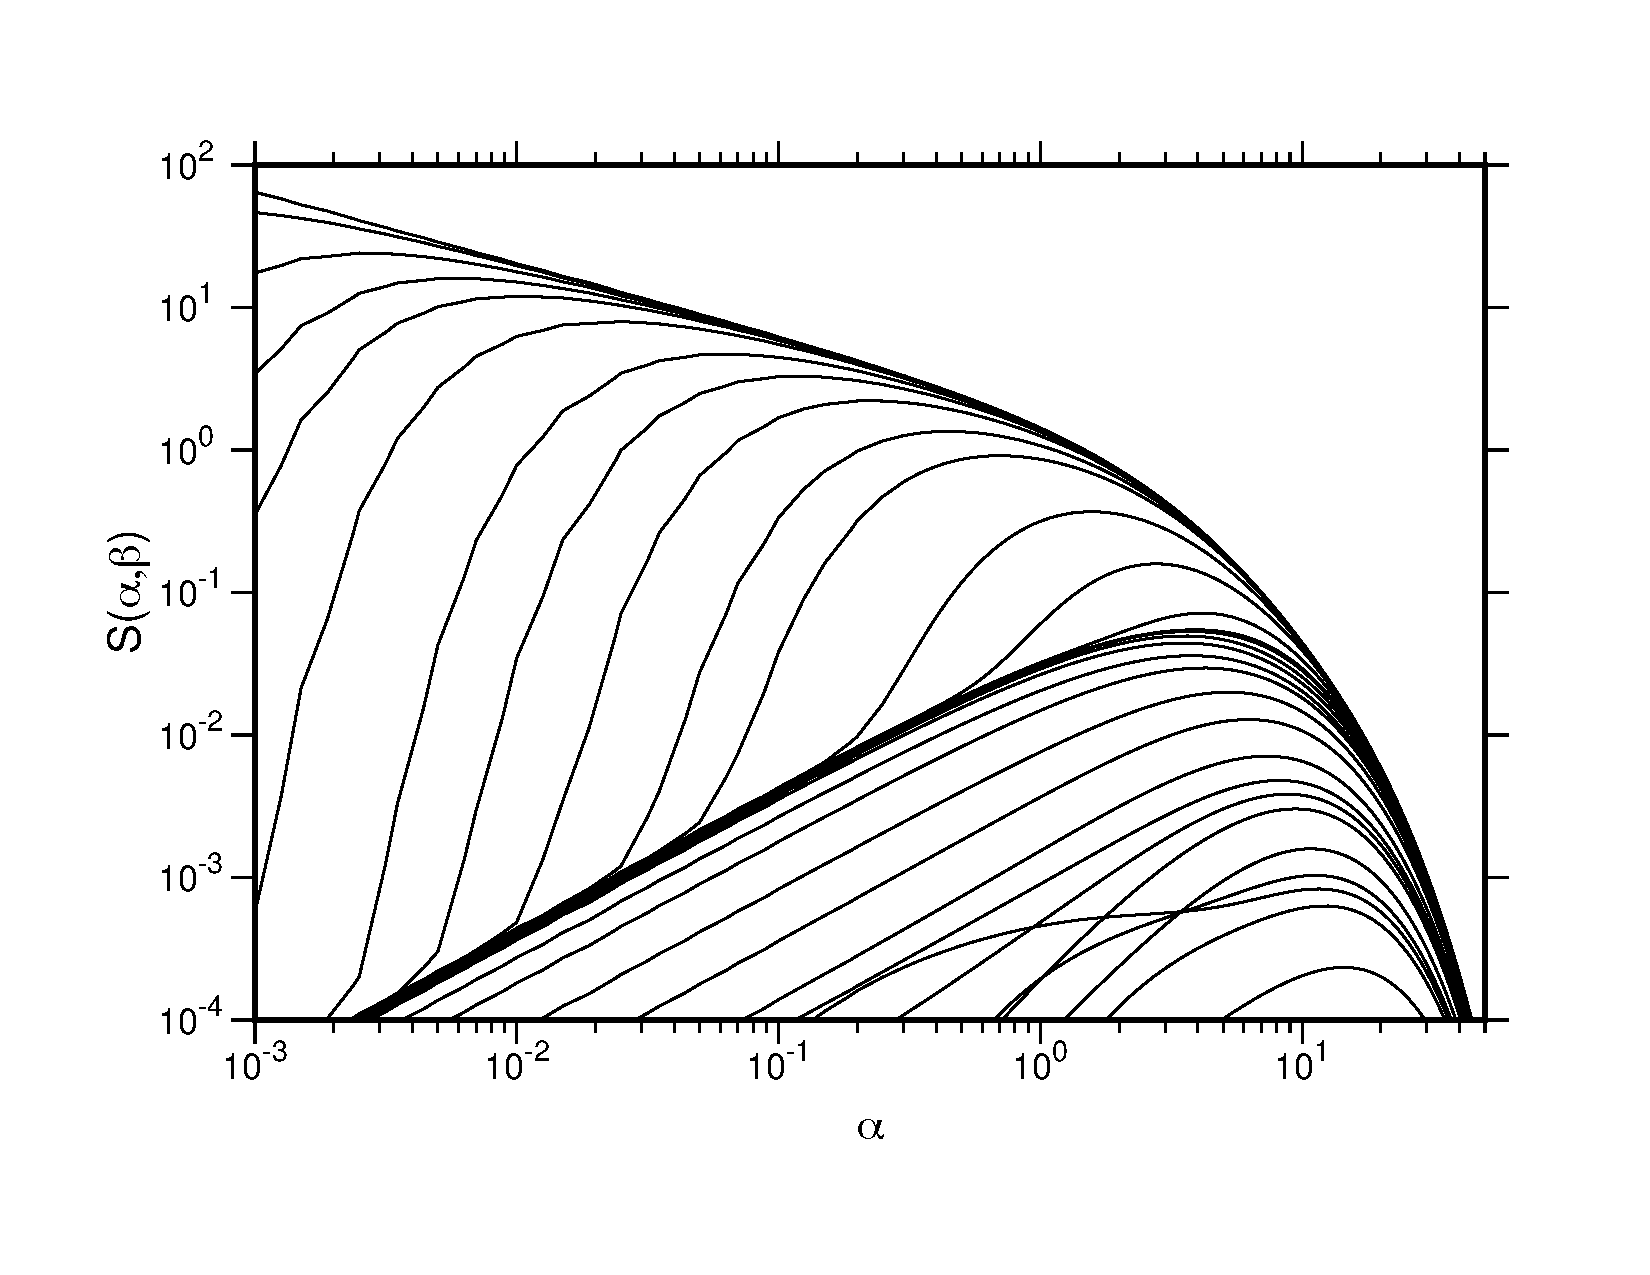
\includegraphics[keepaspectratio, height=3.2in, angle=0]{figs/hh2o-sback}
\caption[S-hat vs beta]
  {${\cal S}(\alpha,-\beta)$ vs $\alpha$ for a number of $\beta$ values.}
\label{hh2o-sb}
\end{figure}

\begin{figure}[b]\centering
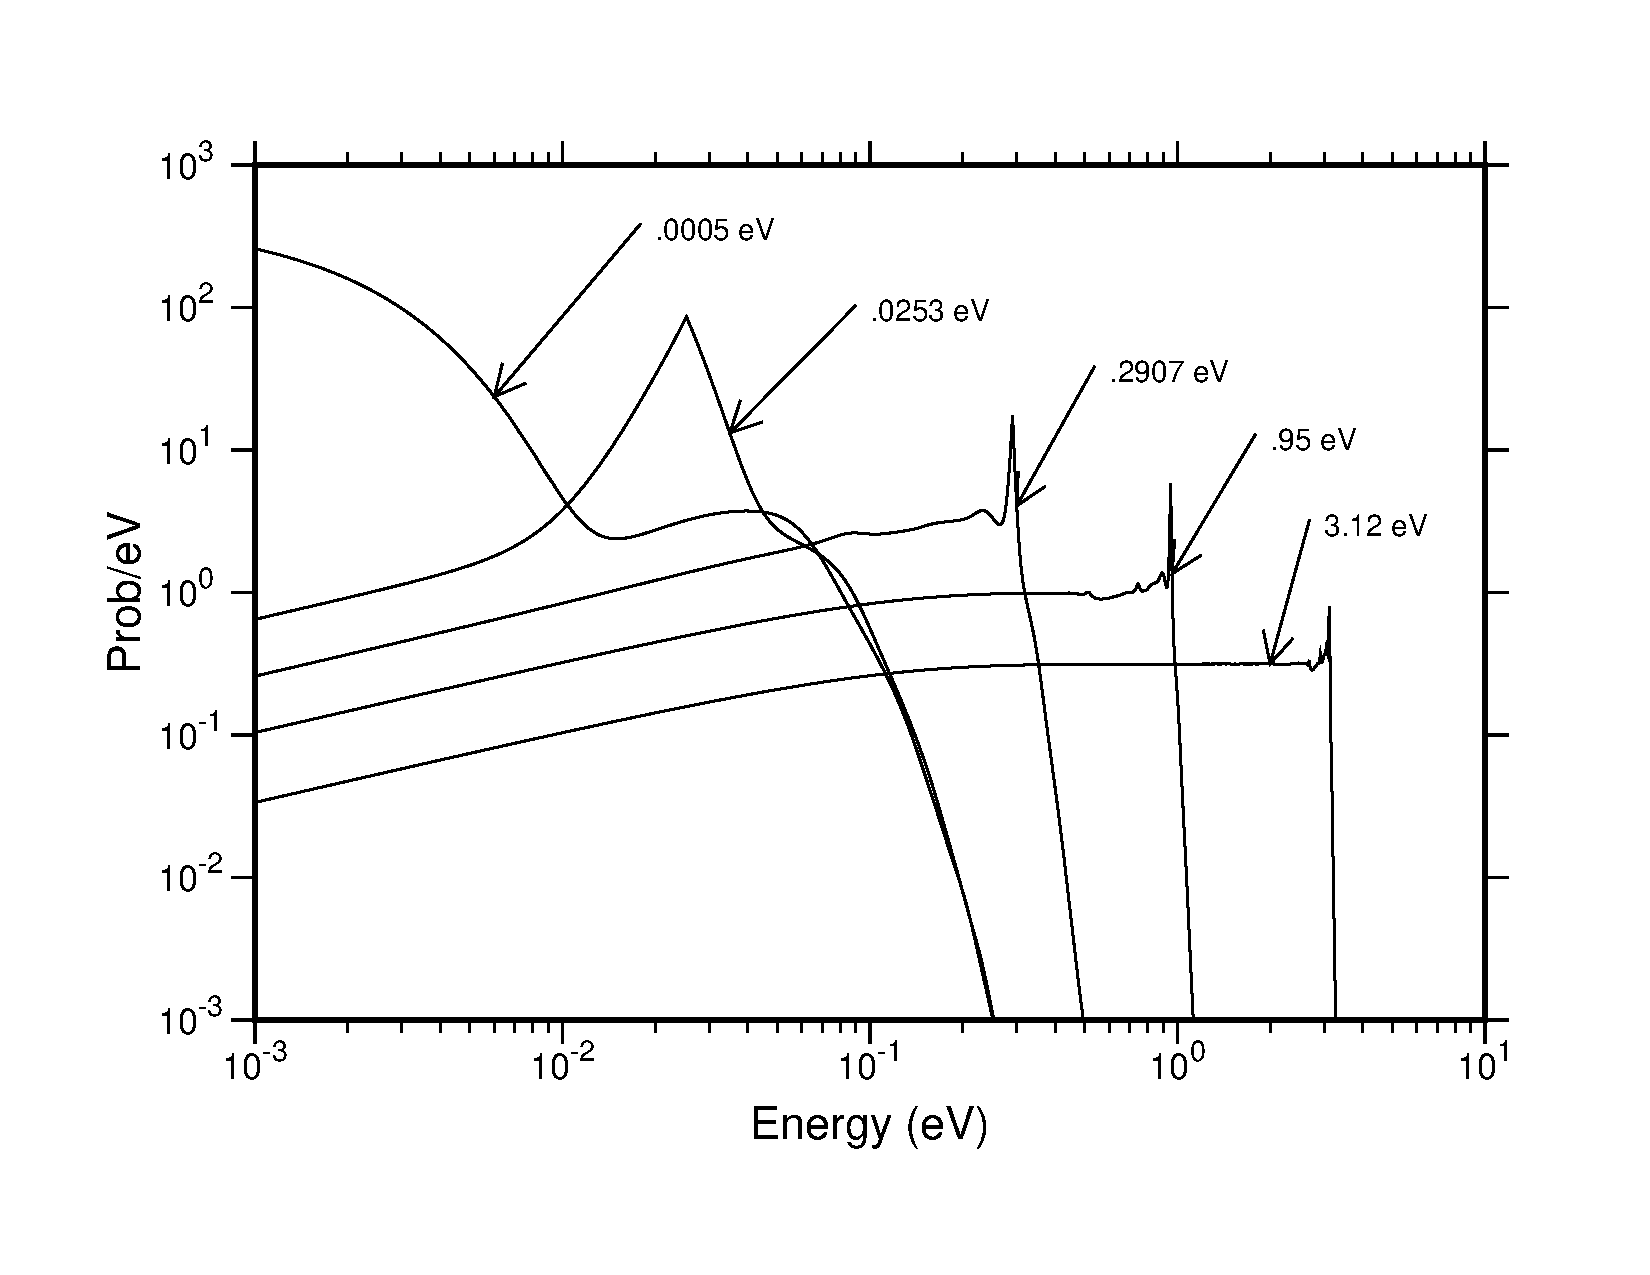
\includegraphics[keepaspectratio, height=3.2in, angle=0]{figs/hh2o-specack}
\caption[Incoherent inelastic spectra for H in H$_2$O]{Incoherent inelastic
 spectra for several incident energies for H in H$_2$O.}
\label{hh2o-spec}
\end{figure}

The neutron emission spectra for incoherent inelastic scattering that
results from processing this scattering law is shown in Fig.~\ref{hh2o-spec}
for several incident energies. For very low incident energies, the neutron
gains energy from the rotational modes excited at thermal equilibrium.
For higher energies, it is more probable that the neutron will lose
energy, and the effects of exciting translational, rotational and
vibrational modes are visible. The down-scatter behavior is shown
in more detail in Fig.~\ref{hh2o-spec2}.  The sharp peak at $E'=E$ is the
quasi-elastic peak coming from the diffusive translations.  The next
lower hump is from rotational modes, and the other peaks are from
vibrational modes.

\begin{figure}[t]\centering
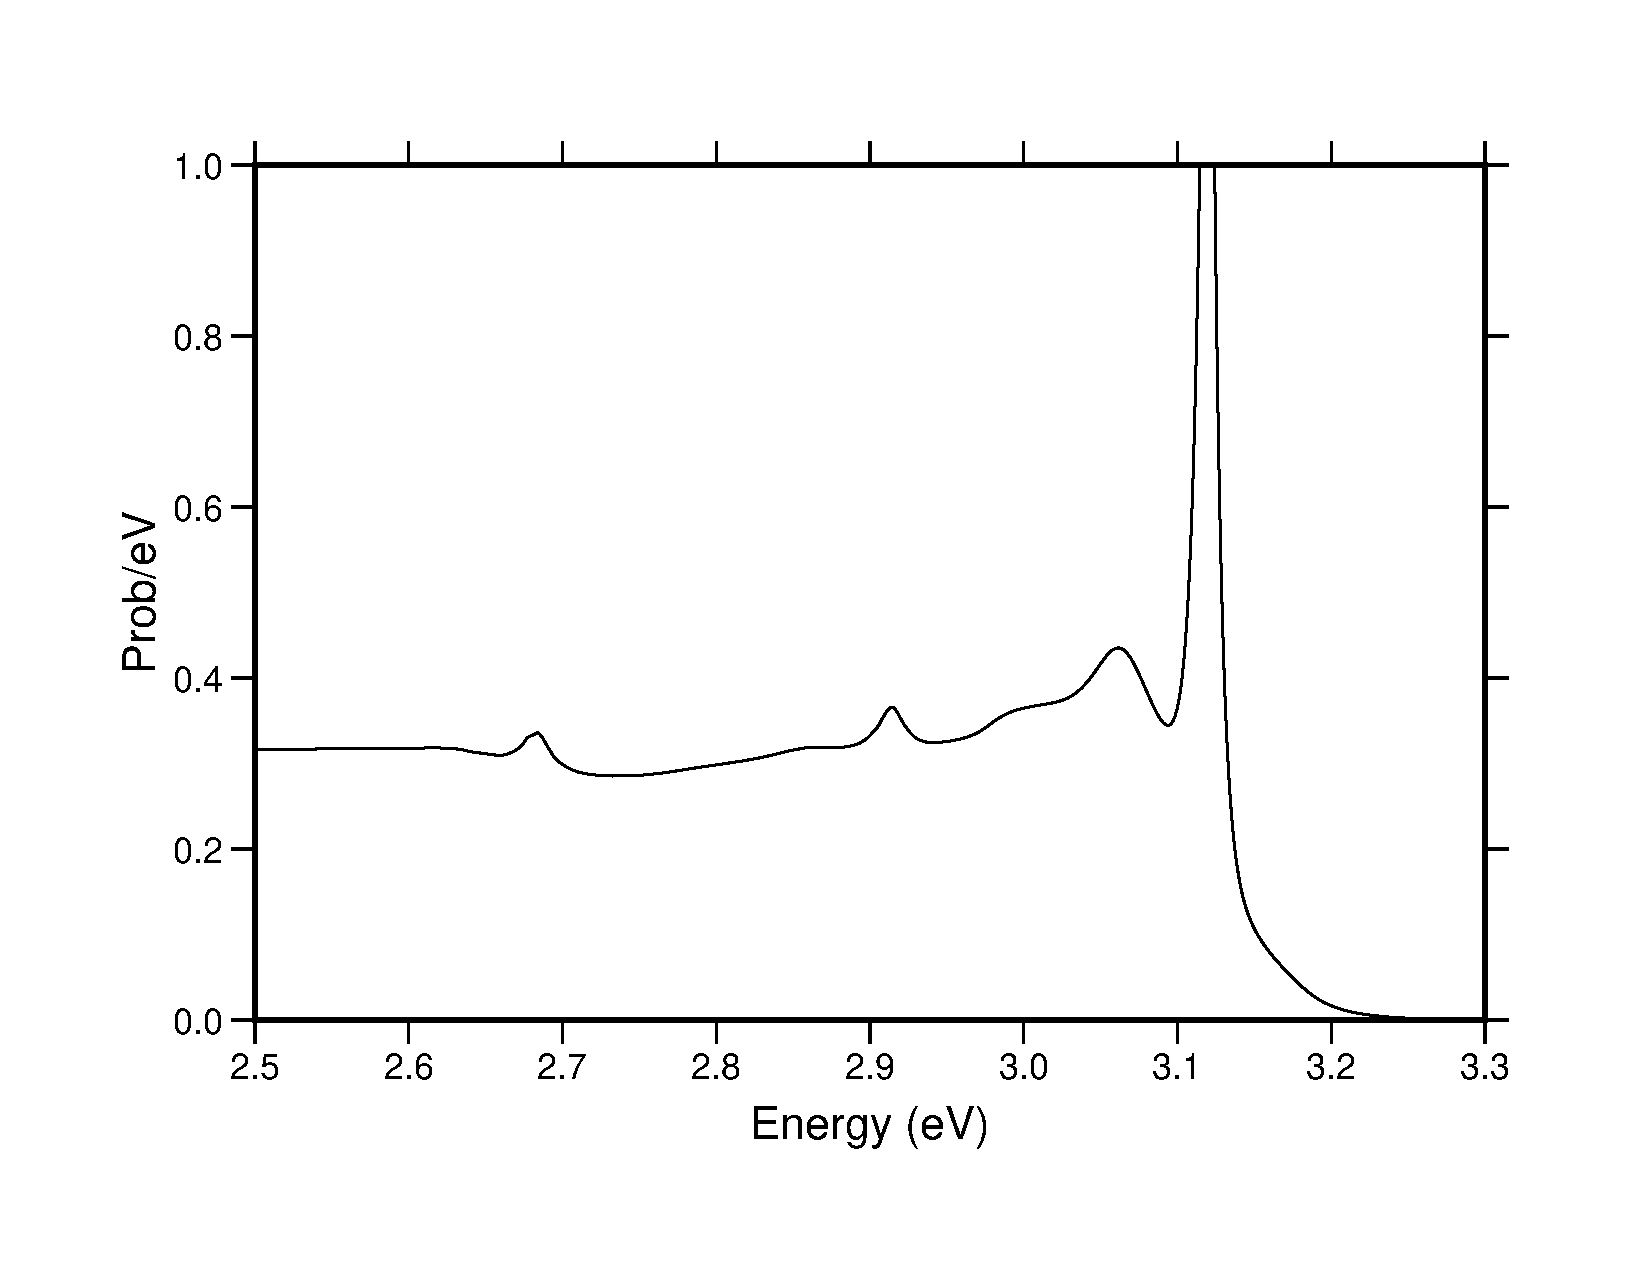
\includegraphics[keepaspectratio, height=3.2in, angle=0]{figs/hh2o-spec2ack}
\caption[Incoherent inelastic spectra for H in H$_2$O, detailed view]{Detailed
 view of a neutron emission spectrum for inelastic scattering for H in H$_2$O.}
\label{hh2o-spec2}
\end{figure}

\begin{figure}[b]\centering
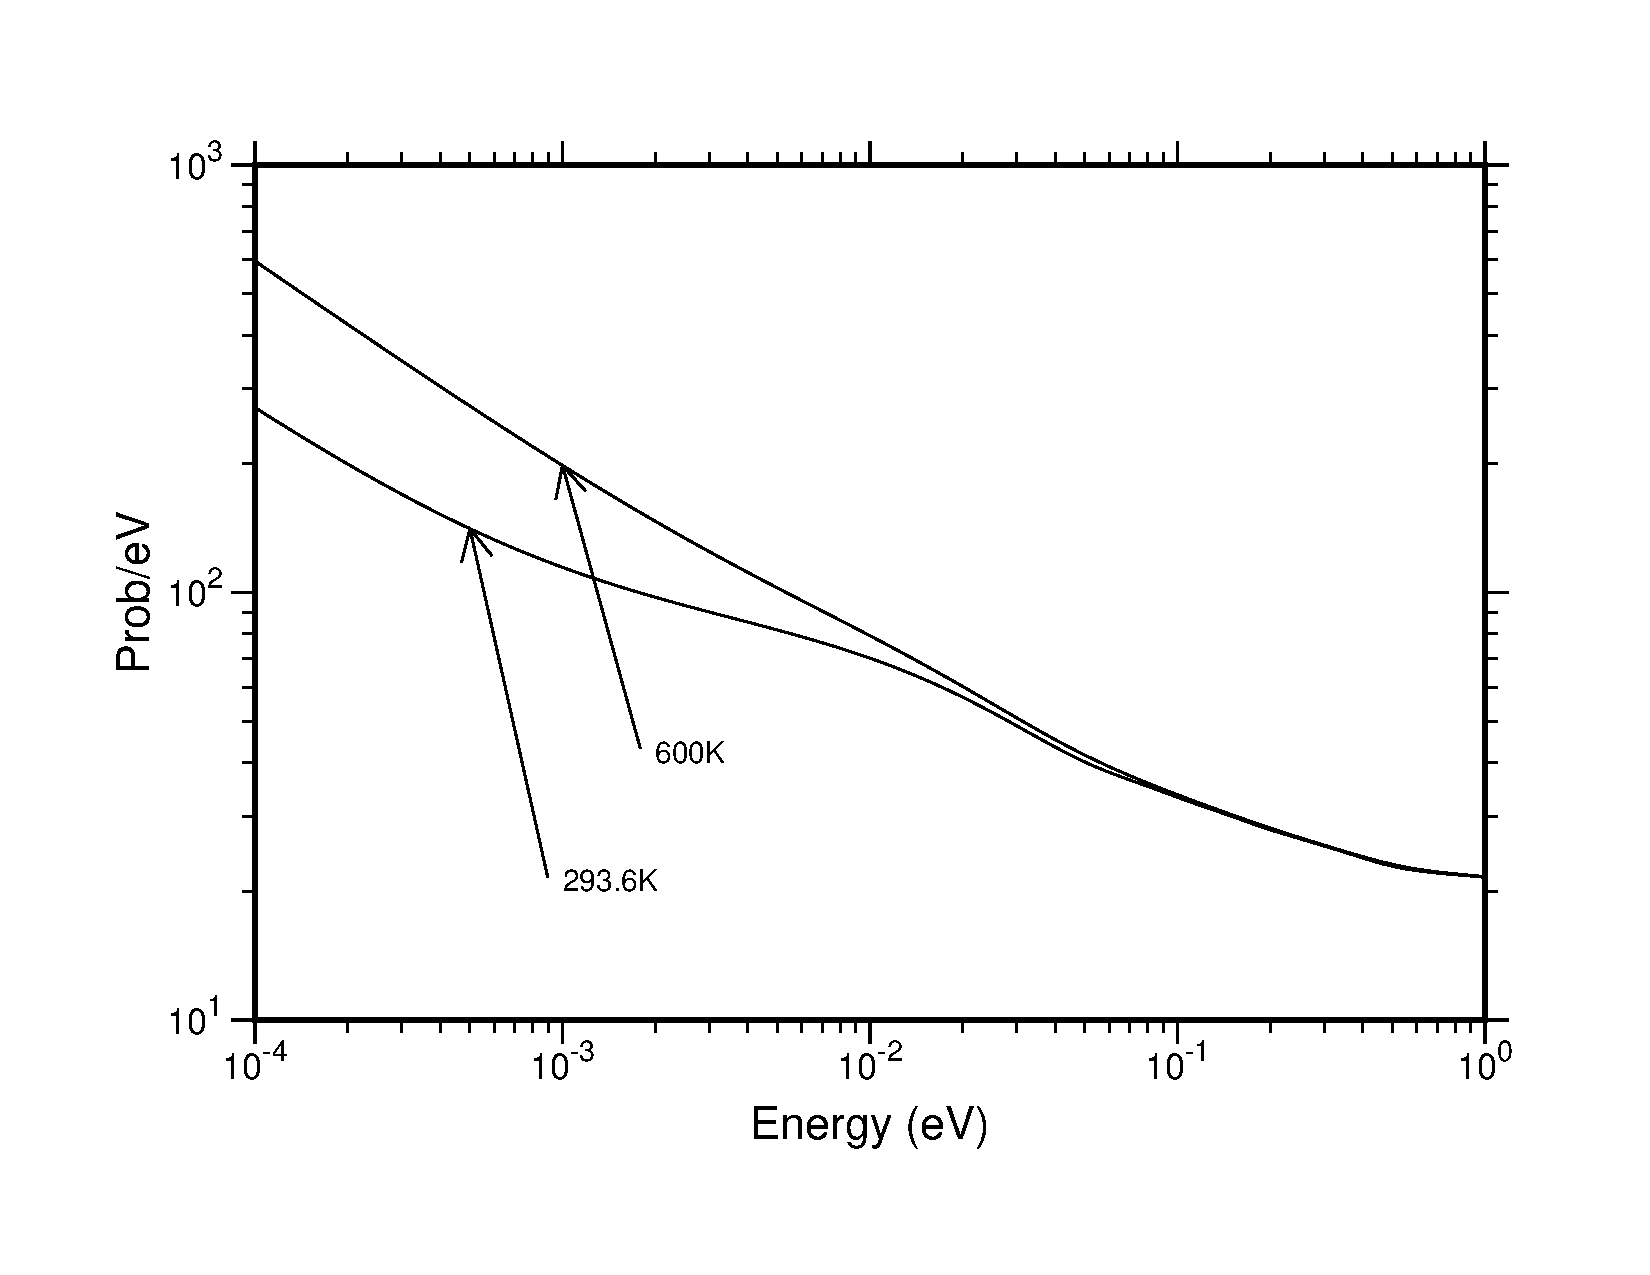
\includegraphics[keepaspectratio, height=3.2in, angle=0]{figs/hh2o-in1ack}
\caption[The incoherent inelastic cross section for H in H$_2$O at two
 temperatures]{The incoherent inelastic cross section for H in H$_2$O
 at two temperatures.}
\label{hh2o-in1}
\end{figure}

The integrated cross section is shown in Fig.~\ref{hh2o-in1} and
Fig.~\ref{hh2o-in2} for two temperatures. As the incident energy
increases, the cross section begins to approach the free-atom value,
as predicted by the theory. In practice, multigroup codes would
normally change from the thermal value to the target-at-rest value
at some particular break-point energy chosen so that error caused
by the additional discontinuity at that energy group was not too
significant. Monte Carlo codes normally change from the thermal
cross section to the free-gas cross section at some breakpoint
energy. There again, it is hoped that the breakpoint can be made
high enough to minimize the adverse effects of the discontinuity.
\index{free atom scattering cross section}
\index{target-at-rest cross section}

\begin{figure}[t]\centering
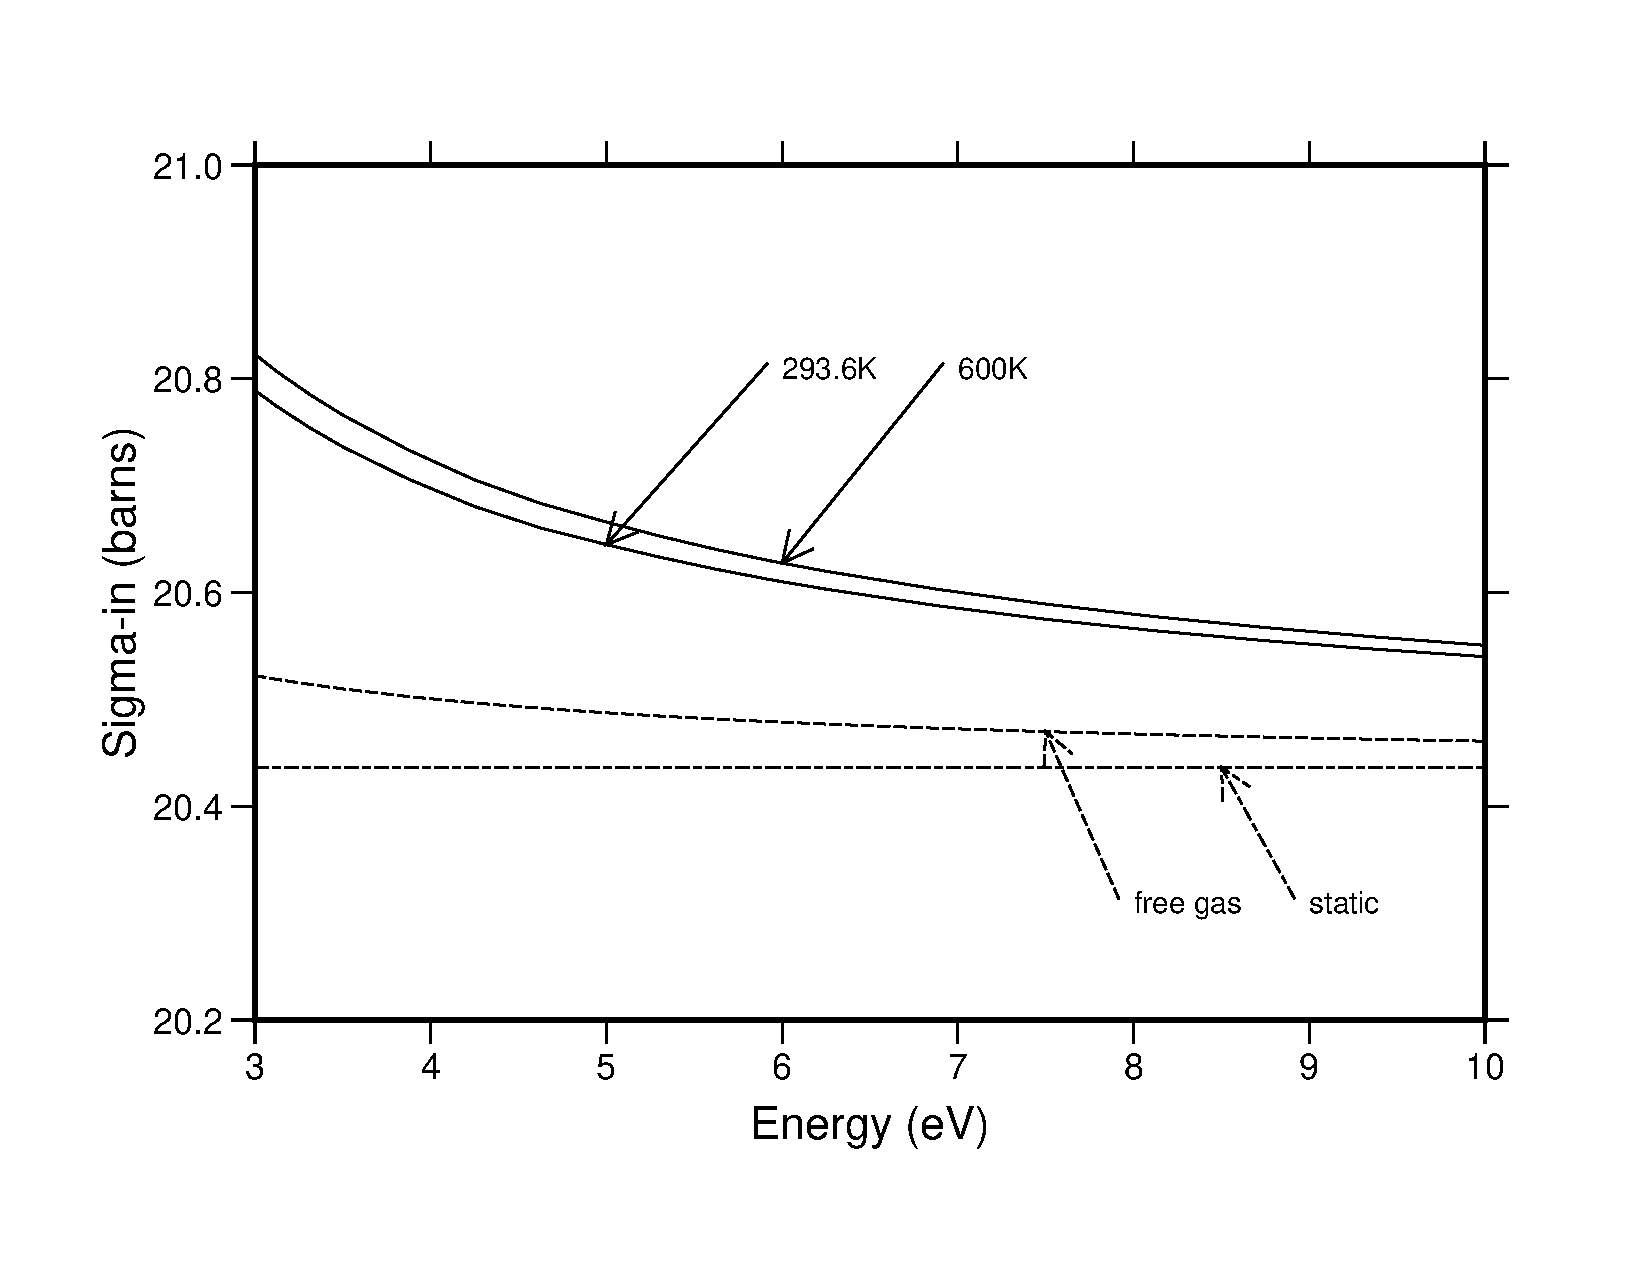
\includegraphics[keepaspectratio, height=3.2in, angle=0]{figs/hh2o-in2ack}
\caption[The incoherent inelastic cross section for H in H$_2$O for higher
 incident energies]{The incoherent inelastic cross section for H in H$_2$O for
 higher incident energies showing the static limit (scattering from atoms at
 rest) and the free-gas cross section.}
\label{hh2o-in2}
\end{figure}

Another approach that has been used in practice is to shift from the
thermal cross section to an SCT cross section, that is, a free-gas
cross section at a higher temperature than the ambient value.
Table~\ref{efft} shows the effective SCT temperatures for H in H$_2$O.
This approach gives a fairly good integrated cross section versus
energy above the thermal cutoff of the scattering law calculation,
and it gives a good downscatter spectrum, but the up-scatter is too large.
\index{SCT|see{short collision time}}

\begin{table}[t]
\begin{center}
\caption[H in H$_2$O SCT effective temperatures]{Effective temperatures
   for the Short Collision Time approximation for H in H$_2$O.}
\label{efft}
\vspace{3mm}
\hspace{-10mm}\begin{tabular}{cc}
\bf\small Temp ($^\circ$K) & \bf\small Eff Temp ($^\circ$K) \\ \hline
293.6 & 1269 \\
350 & 1276 \\
400 & 1289 \\
450 & 1305 \\
500 & 1324 \\
550 & 1344 \\
600 & 1367 \\
800 & 1473 \\ \hline
\end{tabular}
\end{center}
\end{table}
\index{effective temperature}

The angular behavior of thermal scattering is also of interest. For
H bound in H$_2$O, the hydrogen atom is not as free to recoil as the
free atom. This makes it look like it has a higher effective mass,
and it causes the scattering to be more isotropic on the average.
See Fig.~\ref{hh2o-mu}.  However, as Fig.~\ref{hh2oael} demonstrates,
there are still interesting anisotropies seen, especially near $E'=E$
where translational effects are important.
\index{angular distributions}

\begin{figure}[b]\centering
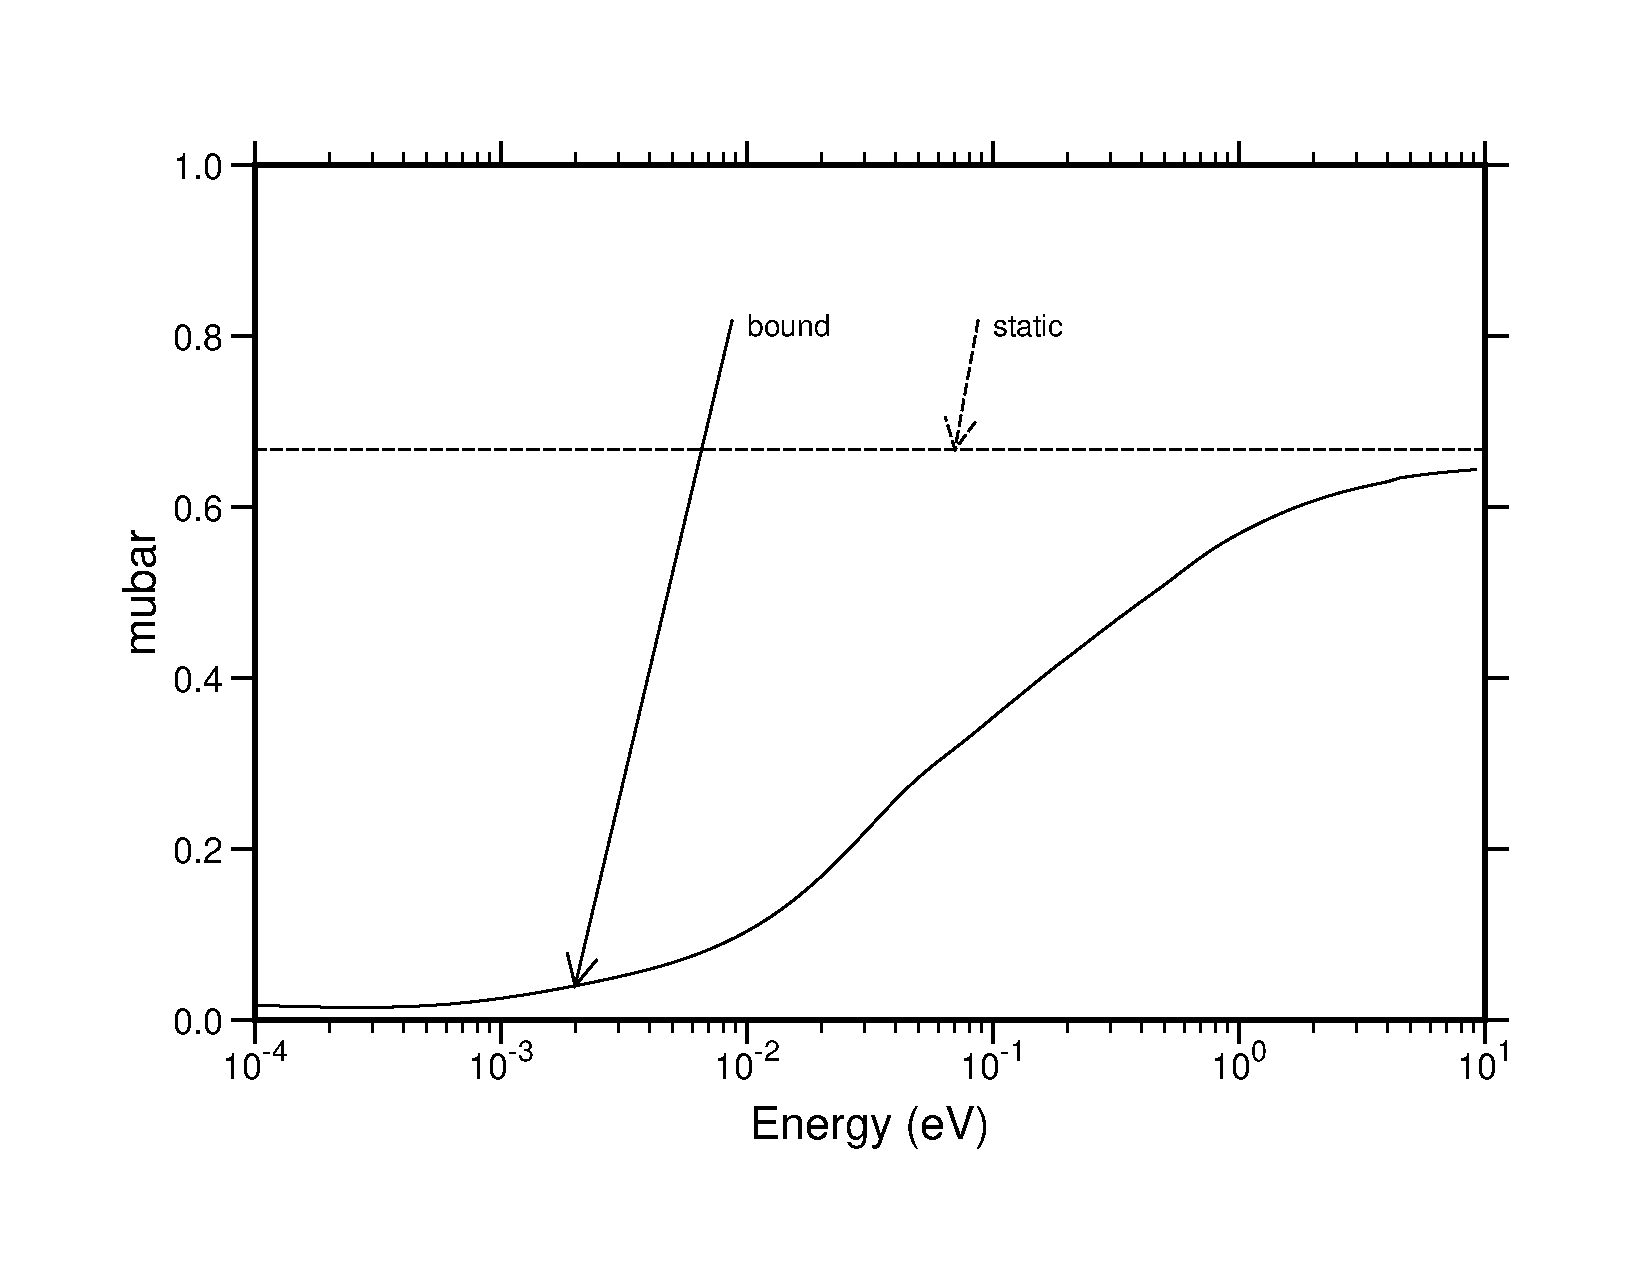
\includegraphics[keepaspectratio, height=3.2in, angle=0]{figs/hh2o-muack}
\caption[The average scattering cosine for H in H$_2$O compared to the
 static value for scattering from atoms at rest]{The average scattering cosine
 for H in H$_2$O compared to the static value for scattering from atoms at
 rest.  The effect of the binding of H in H$_2$O is to make the scattering
 more isotropic at thermal energies.}
\label{hh2o-mu}
\end{figure}

\begin{figure}[p]\centering
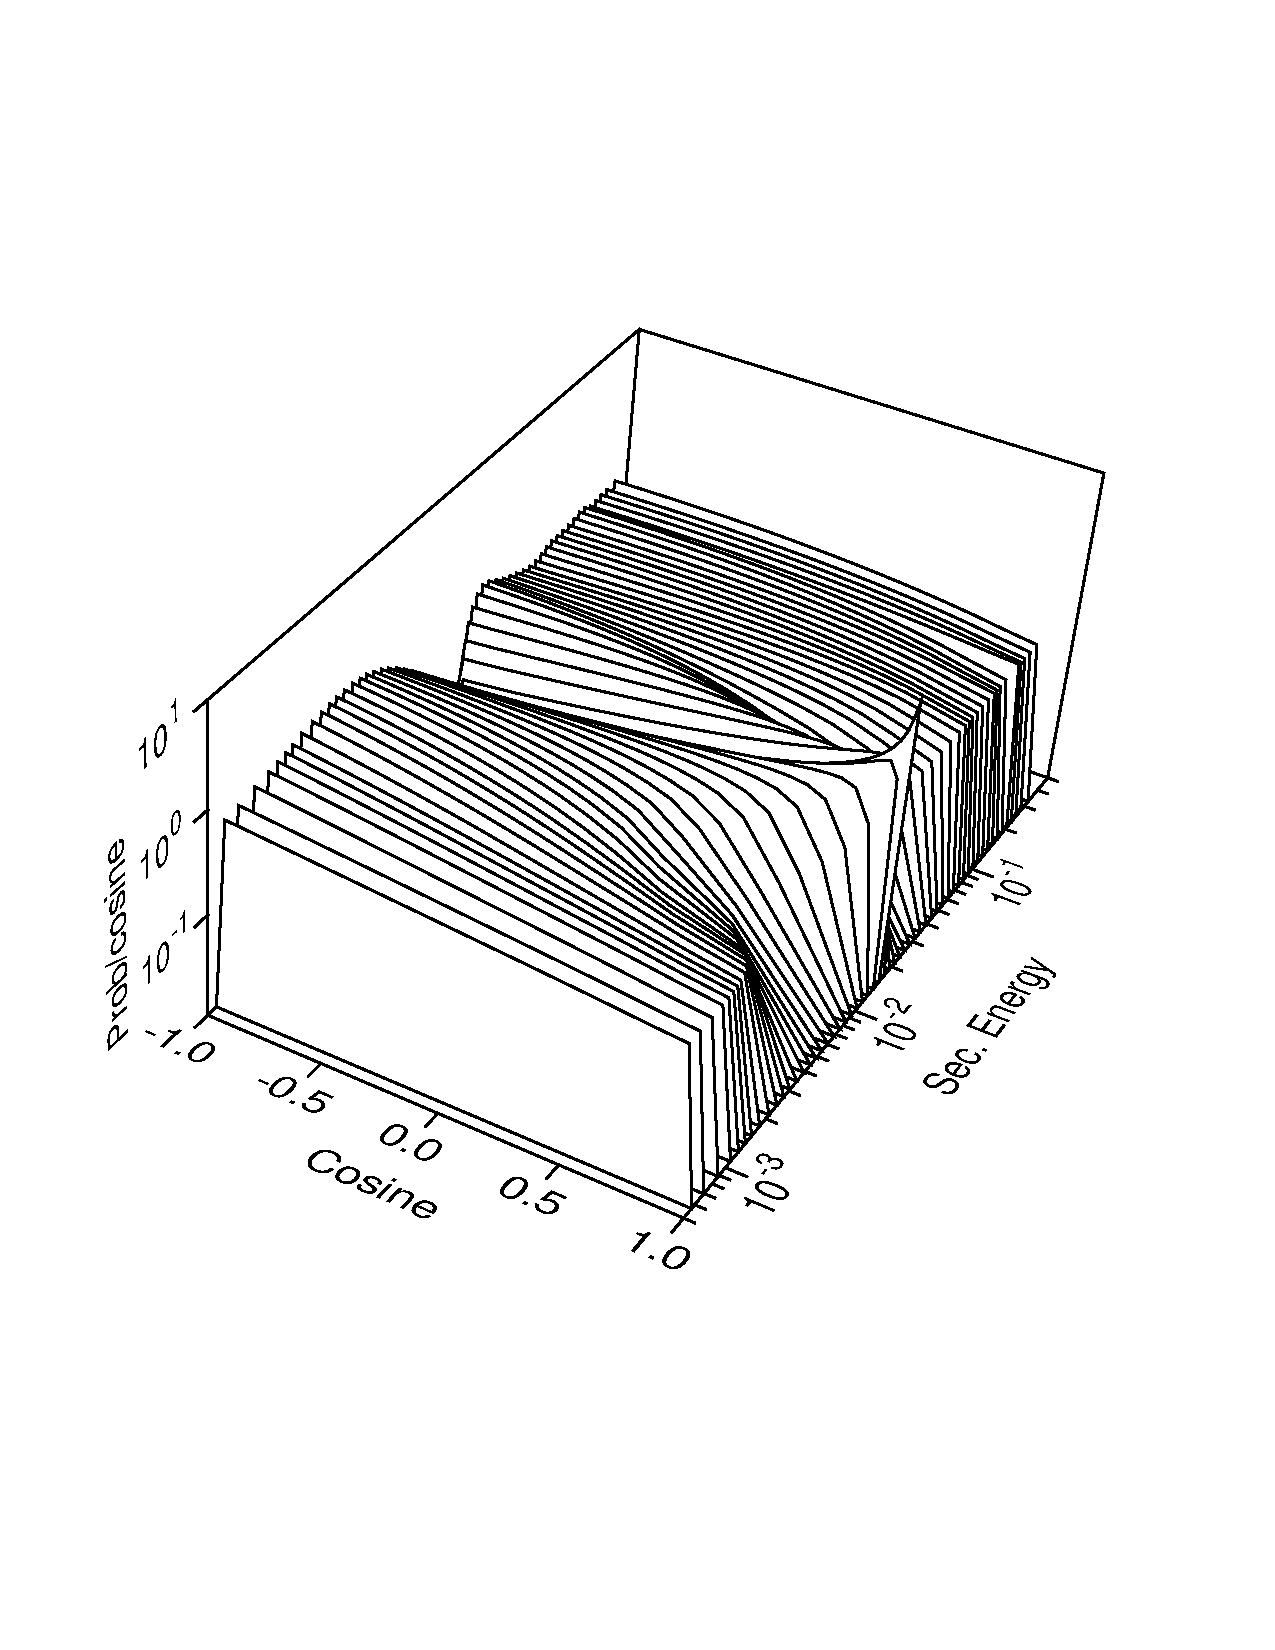
\includegraphics[keepaspectratio, height=3.2in, angle=0]{figs/hh2o-aeack}
\caption[A perspective view of an angle-energy distribution for H in H$_2$O.]
  {A perspective view of an angle-energy distribution for H in H$_2$O.}
\label{hh2oael}
\end{figure}

Fig.~\ref{hh2o-3d} gives an overall view of the isotropic part of the
scattering distribution for H in H$_2$O.

\begin{figure}[p]\centering
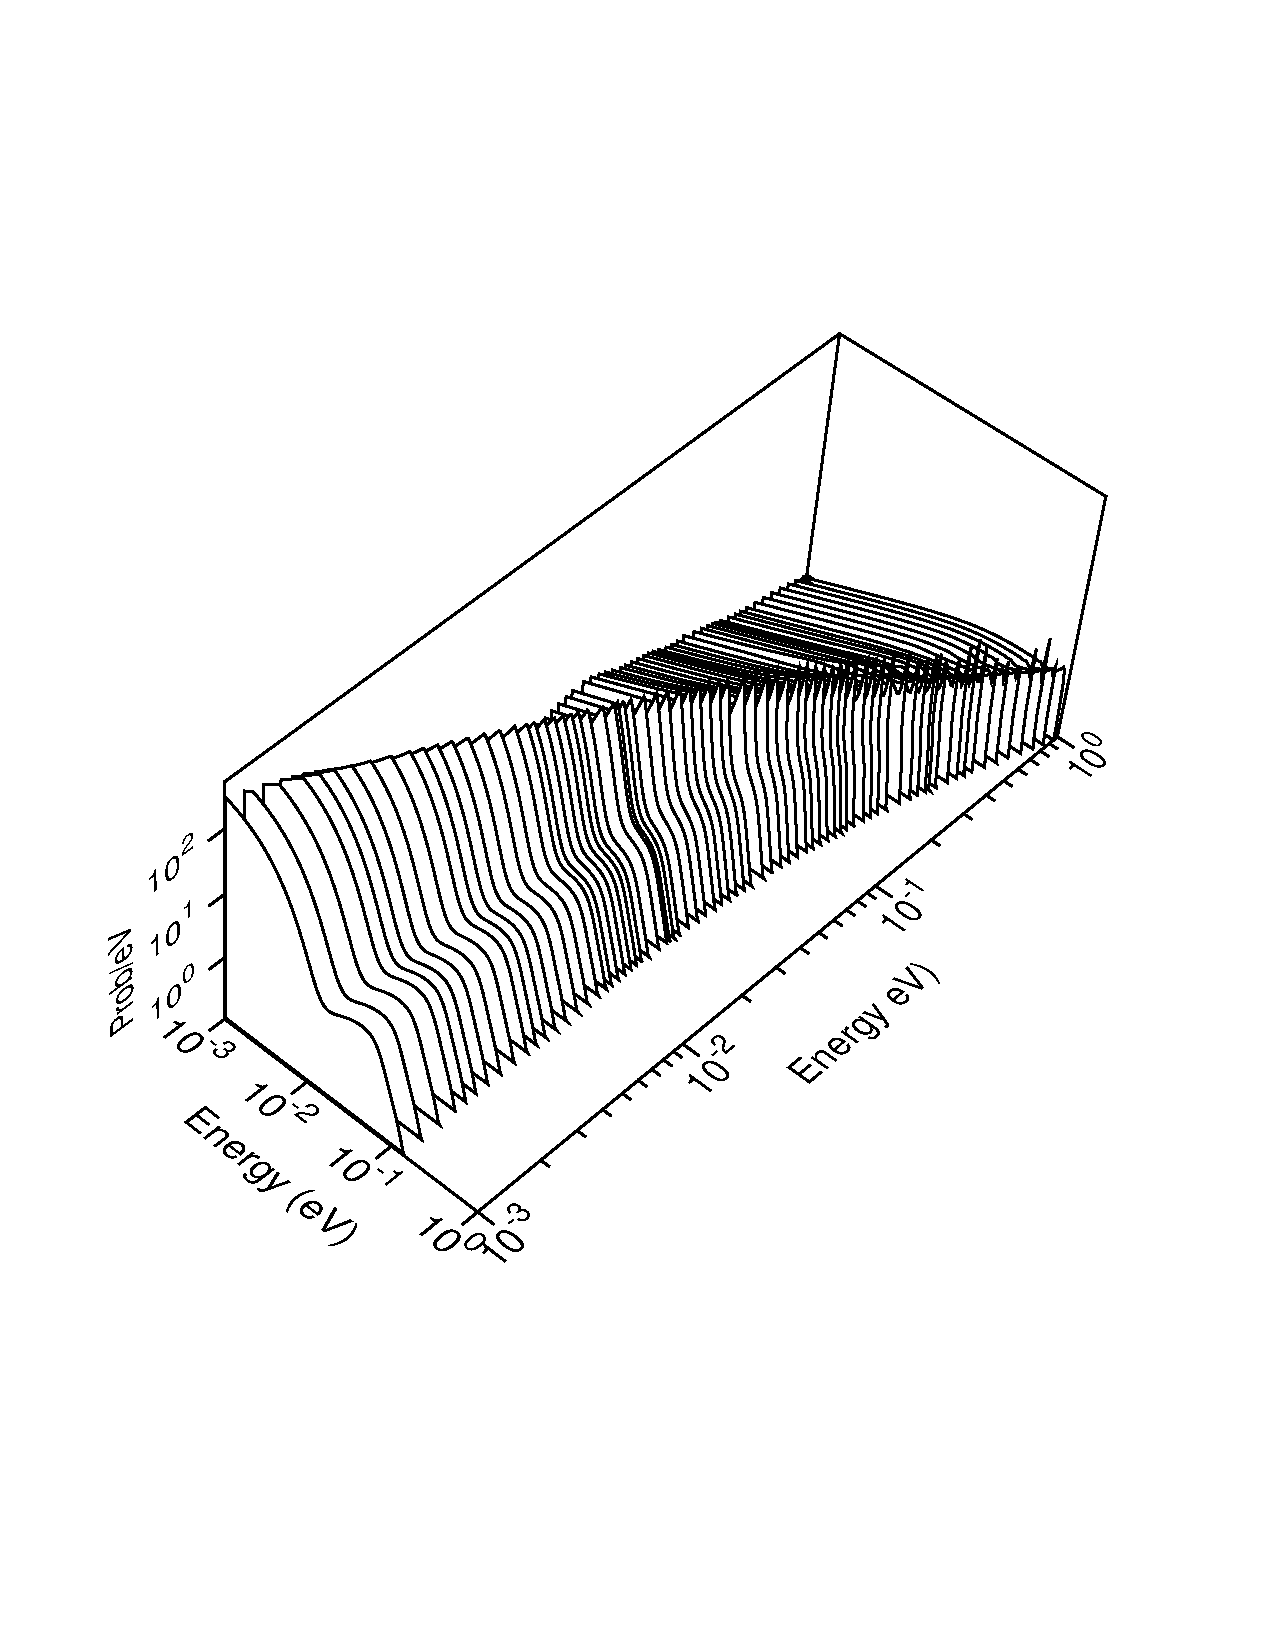
\includegraphics[keepaspectratio, height=3.2in, angle=0]{figs/hh2o-3dack}
\caption[A perspective view of the isotropic part of the incoherent
   inelastic scattering from H in H$_2$O.]
  {A perspective view of the isotropic part of the incoherent
   inelastic scattering from H in H$_2$O.  The variations in the
   size of the quasi-elastic peak are artifacts of the plotting program.}
\label{hh2o-3d}
\end{figure}

As the description of the evaluation for H in H$_2$O demonstrates, ENDF
scattering law data are not obtained directly from experimental
measurement as that requires more complete differential data than
are currently available. Instead, they are modeled based on various
kinds of input data ranging from neutron scattering measurements
to optical results. The model results are then compared to the
available experimental data to see how good of a job was done with the
evaluation. Examples of the comparison of the modeled thermal cross
section for water with
experiment\cite{Dritsa,Heinloth,SmithRR,Walton,Springer,Simpson,Russell}
are shown in Fig.~\ref{hh2o-tot1} and Fig.~\ref{hh2o-tot2}.
Additional comparisons with differential data are shown in the
report on the IAEA evaluation\cite{mattes}.  The results
are fairly good, except around 300 to 400 meV and below 1 meV.
The problem at the lowest energies comes from the failure of the
translational model.  This part of the distribution is not too
important in practice due to effects of detail balance.
\index{measurement vs theory}

\begin{figure}[b]\centering
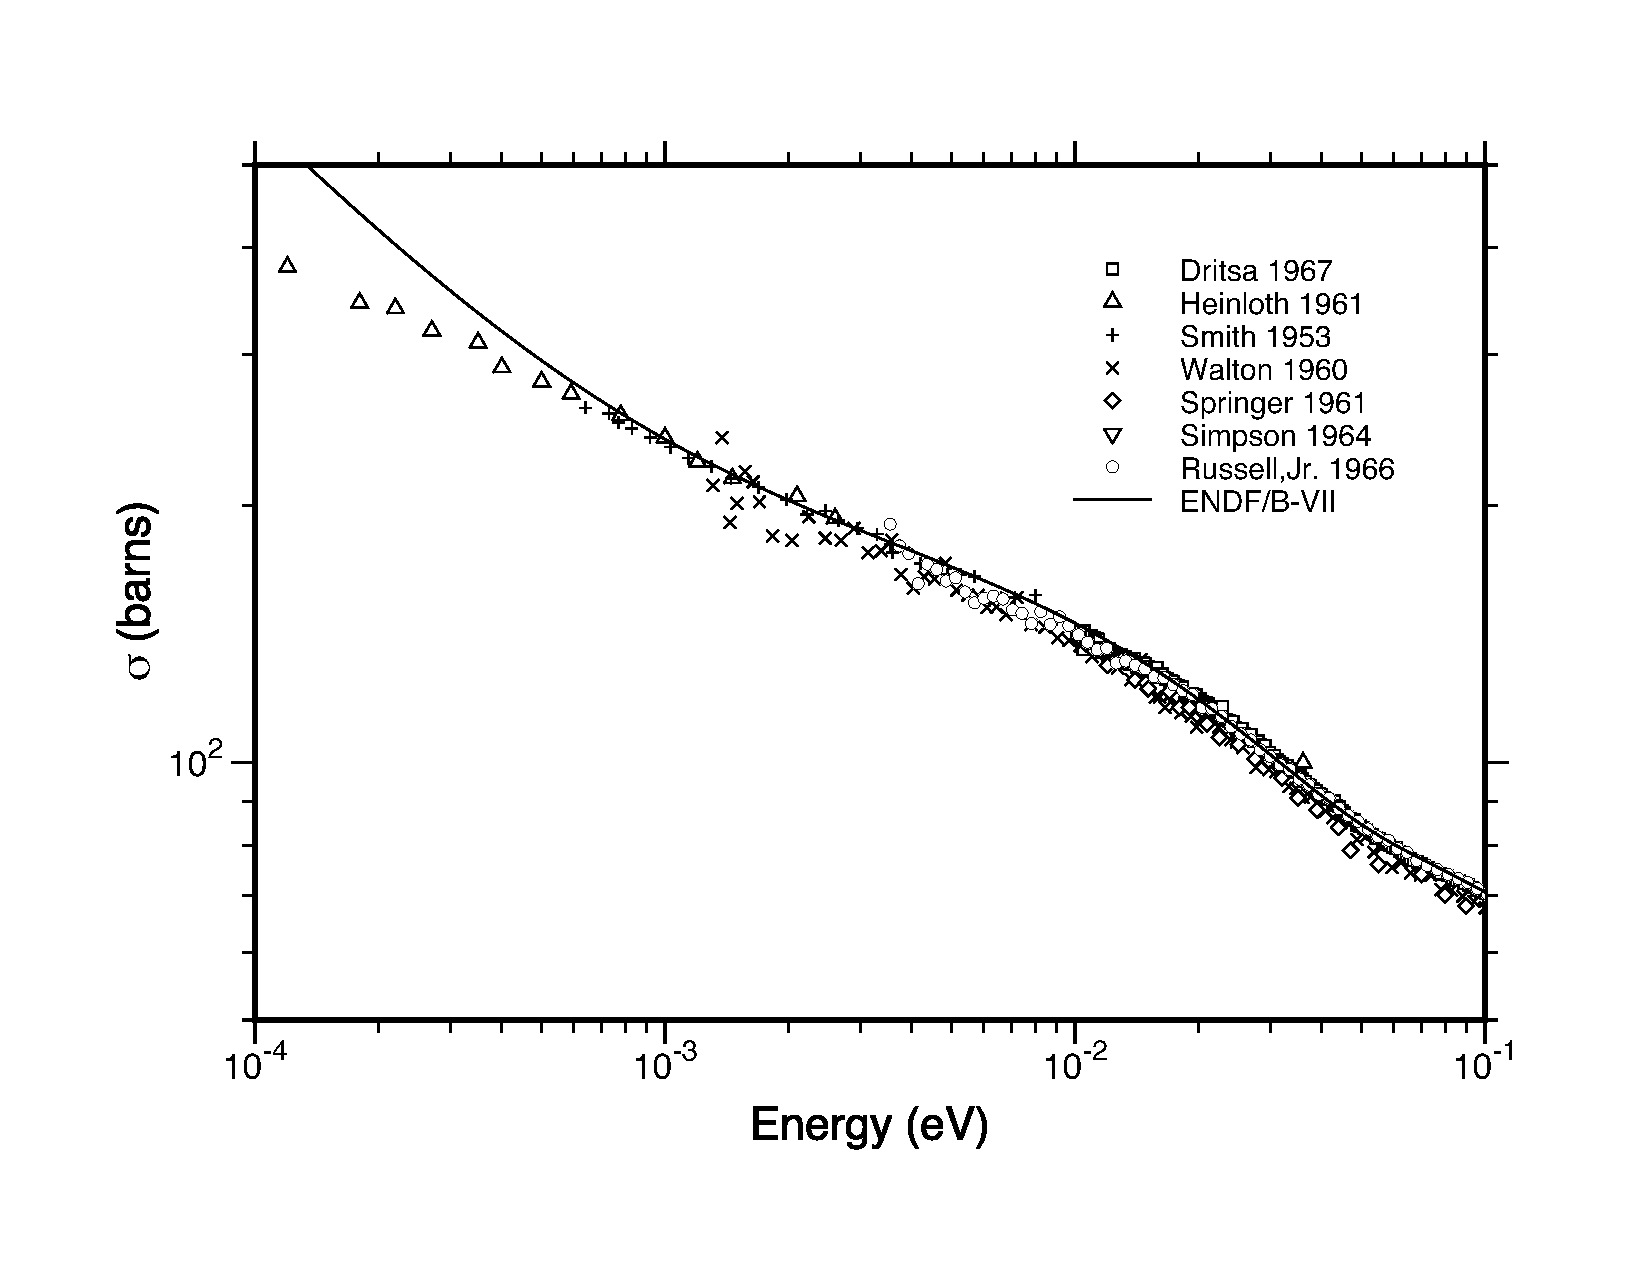
\includegraphics[keepaspectratio, height=3.3in, angle=0]{figs/hh2o-tot1ack}
\caption[Comparison of the ENDF/B-VII.0 thermal cross section for water at
 lower incident energies with experimental results]{Comparison of the
 ENDF/B-VII.0 thermal cross section for water at lower incident energies
 with experimental results for the CSISRS compilation at the the National
 Nuclear Data Center of the Brookhaven National Laboratory.  See the
 compilation for the references.}
\label{hh2o-tot1}
\end{figure}
\index{CSISRS compilation}
\index{National Nuclear Data Center!NNDC}

\begin{figure}[t]\centering
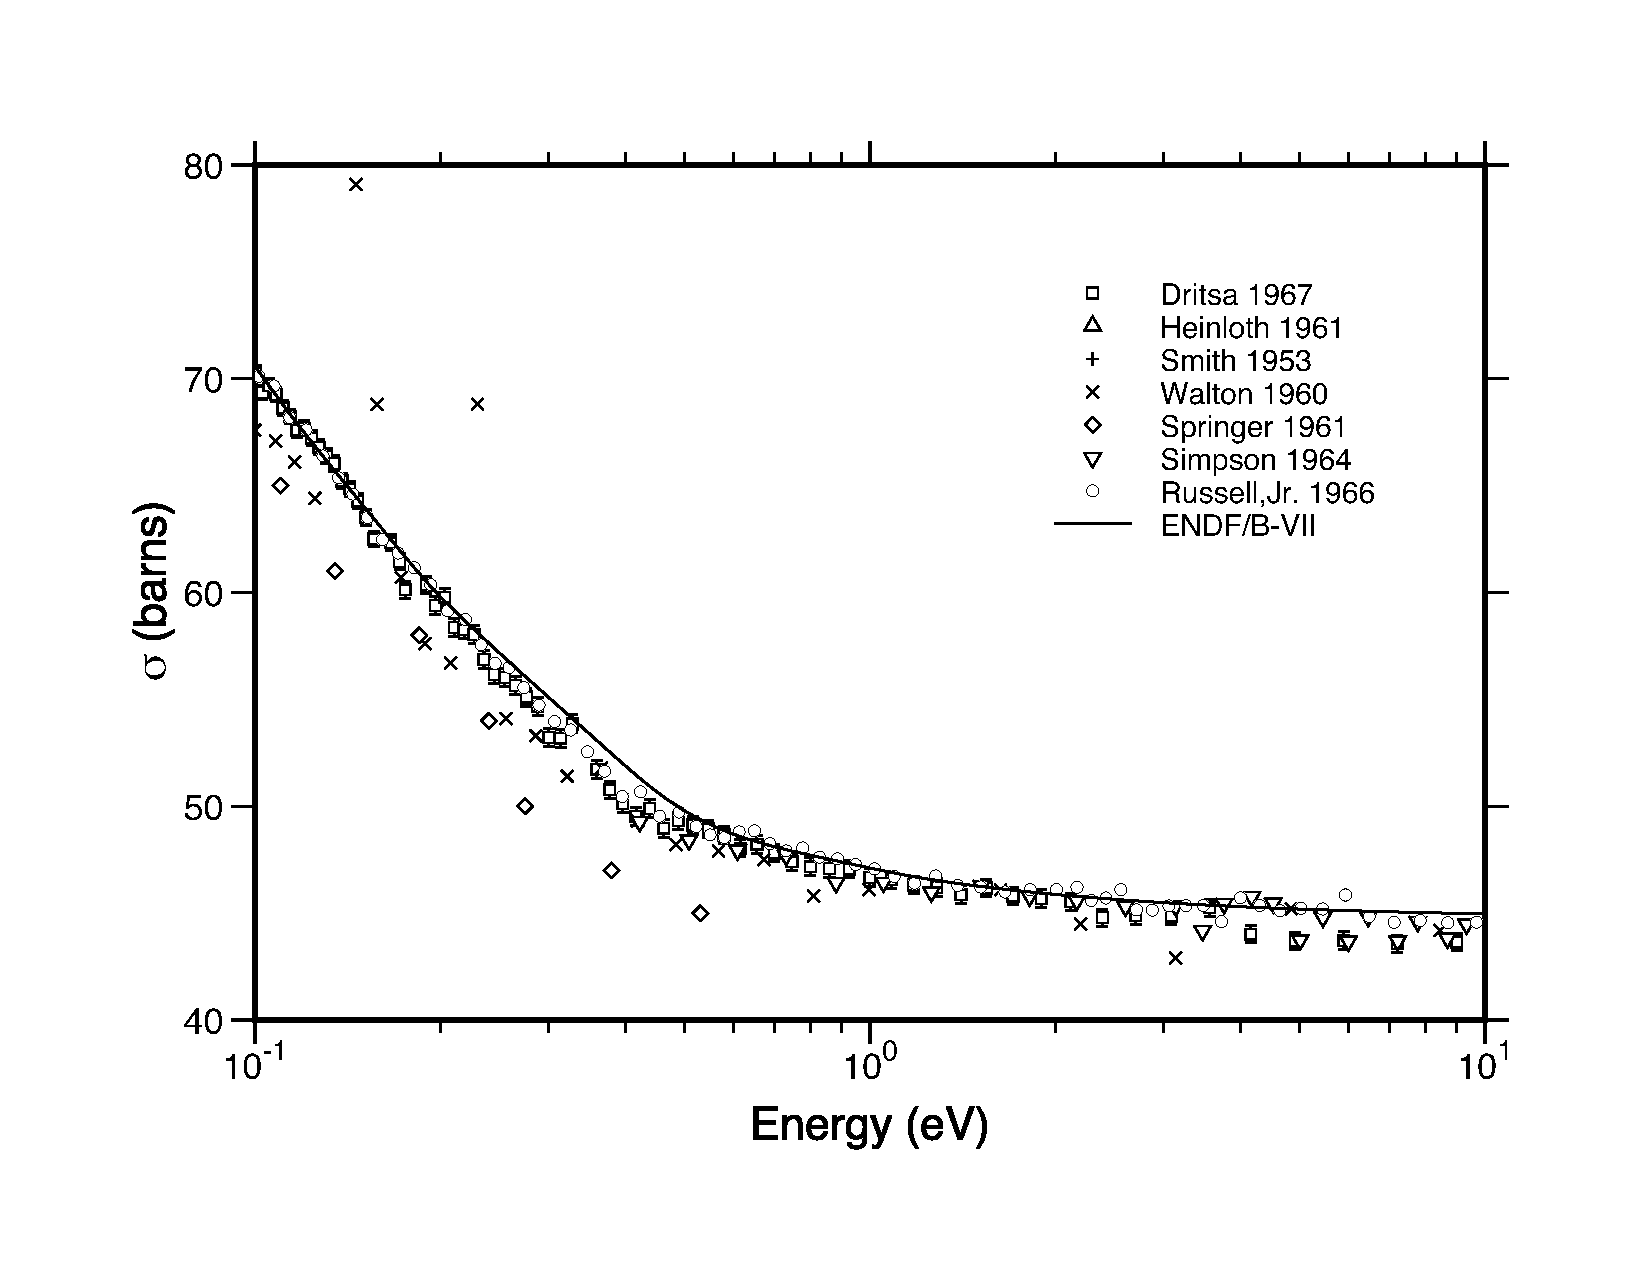
\includegraphics[keepaspectratio, height=3.0in, angle=0]{figs/hh2o-tot2ack}
\caption[Comparison of the ENDF/B-VII.0 thermal cross section for water at
 higher incident energies with experimental results]{Comparison of the
 ENDF/B-VII.0 thermal cross section for water at higher incident energies
 with experimental results for the CSISRS compilation at the the National
 Nuclear Data Center of the Brookhaven National Laboratory.  See the
 compilation for the references.}
\label{hh2o-tot2}
\end{figure}

\paragraph{The Model for Solid Methane.}
The methane molecule consists of an atom of carbon surrounded by four
atoms of hydrogen placed on the corners of a tetrahedron.  The carbon
atom is at the center of mass of the system; because of its symmetry,
the methane molecule is often called a ``spherical top".  Optical
measurements of methane in the gas phase show four fairly well defined
vibrational modes at 162 meV, 190 meV, 361 meV and 374 meV.  Following the lead
of Picton, they have been included in this model as discrete oscillators
with weights equal to .308, .186, .042, and .144, respectively.

Specific heat measurements in solid methane near one atmosphere show
three phases with transitions at 8K and 20.4K.  The melting point is
about 89K.  X-ray measurements show that the carbon atoms are
arranged on an fcc lattice for both of the higher two phases; it has
been speculated that the phase transition is due to a change in the
degree of rotational order, or perhaps due to the onset of a
self-diffusion behavior.  Because of this interesting question, a
series of slow neutron inelastic scattering experiments were carried
out with samples in each of the phases\cite{HB}.  Since hydrogen is
an incoherent scatterer, it was possible to analyze the data to obtain
a frequency spectrum for hydrogen in solid methane.  The results didn't
really explain what was happening in the 20K phase transition, but they
did provide the data needed for our calculation.

Again following Picton, we chose the spectrum for 22.1K for our model.
Instead of using Picton's numbers directly, we digitized the curve from
the graph in the reference, plotted it on a large scale, and then
smoothed it by hand.  Care was taken to use an $\omega^2$ variation
for low energies.  The resulting spectrum is shown in Fig.~\ref{smethr}.
As discussed by Harker and Brugger, the appropriate normalization for
this curve is 0.32.

\begin{figure}[t]\centering
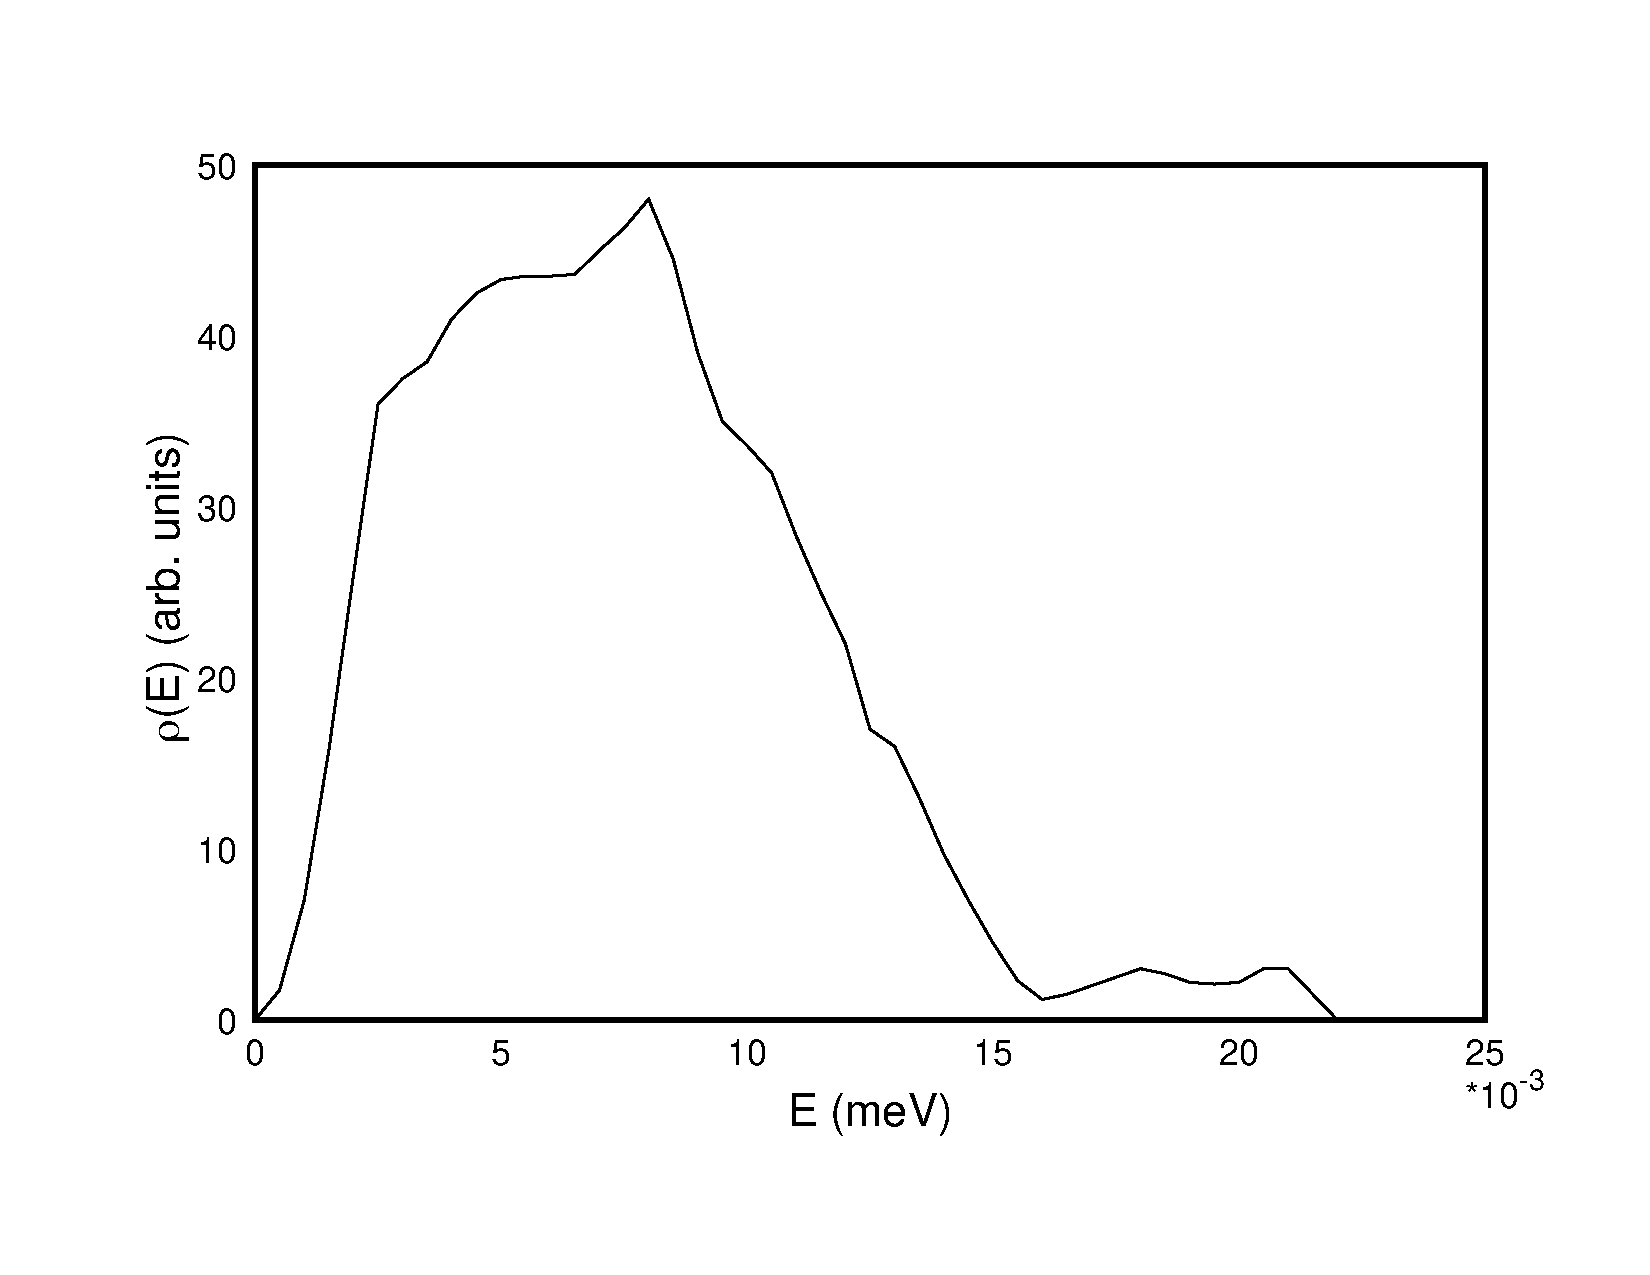
\includegraphics[keepaspectratio, height=3.2in, angle=0]{figs/le1ack}
\caption[Harker-Brugger frequency spectrum used for solid methane]{The
 Harker-Brugger frequency spectrum used for solid methane.  Note the
 quadratic shape at low energies.}
\label{smethr}
\end{figure}

This spectrum and the four discrete oscillators were then used to
calculate $S(\alpha,\beta)$ with LEAPR using the $\alpha$ and $\beta$
grids of Picton.  The input file follows:

\small
\begin{ccode}

leapr
26/
'solid methane at 22K, Harker & Brugger spectrum'/
 1 2/
 11 1001./
 0.9992 20.36 4/
 1 1. 11.898 4.7392 1/
 70 80/
 .1742 .3488 .4059 .4644 .5215 .6386 .7547 .8703
   .9860 1.1601 1.3932 1.6245 1.9148 2.2050 2.6105
   3.0177 3.5393 4.1198 4.8740 5.6871 6.6159 7.7760
   9.0522 10.6200 12.4187 14.5066 16.9443 19.8464 23.2115
   27.0995 31.7421 37.0805 43.4052 50.7168 59.1889 69.6343
   81.2403 87.0431 94.0059 101.5493 110.2545 120.1198 129.9834
   151.4547 177.5682 188.0122 204.2604 207.1629 209.4831 214.7058
   217.0265 220.5090 232.1145 242.5599 261.1291 272.7347 282.0199
   287.2413 298.2667 304.6496 311.0342 319.1575 327.2810 331.9236
   350. 370. 390. 410. 450. 500./
 0. .1742 .3488 .4059 .4644 .5215 .6386 .7547 .8703
   .9860 1.1601 1.3932 1.6245 1.9148 2.2050 2.6105
   3.0177 3.5393 4.1198 4.8740 5.6871 6.6159 7.7760
   9.0522 10.6200 12.4187 14.5066 16.9443 19.8464 23.2115
   27.0995 31.7421 37.0805 43.4052 50.7168 59.1889 69.6343
   81.2403 85.451 89.650 94.0059 96.0 100.221 104.6 110.2545
   120.1198 129.9834 151.4547 170.90 177.5682 181.6 185.67 190.419
   193.8 197.276 200.8 204.2604 207.1629 209.4831 214.7058
   217.0265 220.5090 232.1145 242.5599 261.1291 272.7347 282.0199
   287.2413 298.2667 304.6496 311.0342 319.1575 327.2810 331.9236
   350. 370. 390. 410. 430. 450./
 22/
 .0005 45/
 0. 1.75 7 15.75 26 36 37.5 38.5 41 42.5 43.3 43.5
  43.5 43.6 45 46.3 48 44.5 39 35 33.6 32 28.3 25 22 17 16
  13 9.7 7 4.5 2.3 1.2 1.5 2 2.5 3 2.7 2.2 2.1 2.2 3 3 1.5
  0./
 0. 0. .32/
 4/
 .162 .190 .361 .374/
 .308 .186 .042 .144/
' S-CH4     LANL       EVAL-NOV92 MACFARLANE'/
' NO REF TO DATE       DIST-'/
'----ENDF/B-6          MATERIAL 11'/
'-----THERMAL DATA'/
'------ENDF-6'/
' SOLID METHANE AT 22K, SPECTRUM OF HARKER AND BRUGGER.'/
/
stop

\end{ccode}
\normalsize

After the calculation, the moments of $T_n$ and $S(\alpha,\beta)$ can be
checked.  The errors should be modest.  The output listing for the
solid-type part of the problem should be examined carefully to see that the
$\alpha$ and $\beta$ ranges are sufficient and that the normalization
and sum rule checks are reasonably well satisfied.   Since this is a
solid, there was no translational calculation.  In the discrete-oscillator
calculation the delta functions for $\beta>0$ are put directly into the
scattering law as sharp triangles.  The $\beta{=}0$ peak is converted
into incoherent elastic scattering.   A listing showing some of the
discrete lines is given below:

\newpage
\small
\begin{ccode}

   alpha=   2.61050

      debye-waller factor=  6.0347e-01

      discrete lines
              beta      weight
             0.000  9.8340E-01
           -85.451  9.2531E-03
          -170.903  4.3532E-05
          -100.221  4.7644E-03
          -185.672  4.4830E-05
          -200.441  1.1541E-05
          -190.419  5.6623E-04
          -197.276  1.8739E-03
          -282.728  1.7632E-05
        norm check    1.0000
        rule check    0.9964

\end{ccode}
\normalsize

\noindent
The Debye-Waller factor printed here is the one from the solid-type
spectrum, $\lambda_s$.  It defines the total strength of all the
discrete lines.  All the discrete lines taken together must satisfy
the normalization and sum-rule requirements of any scattering law.
If the number of discrete lines increases above 100, some of them will
begin to be lost, and the checks will begin to decrease below unity.
The listing for the discrete-oscillator calculation should show that the
grid specified does a reasonable job of satisfying the overall
normalization and sum-rule checks.  LEAPR automatically prepared an
output file in ENDF-6 format.  Plots of $S(\alpha,\beta)$ {\it vs.}
$\beta$ for several values of $\alpha$ are give in Fig.~\ref{smeths}.

\begin{figure}[t]\centering
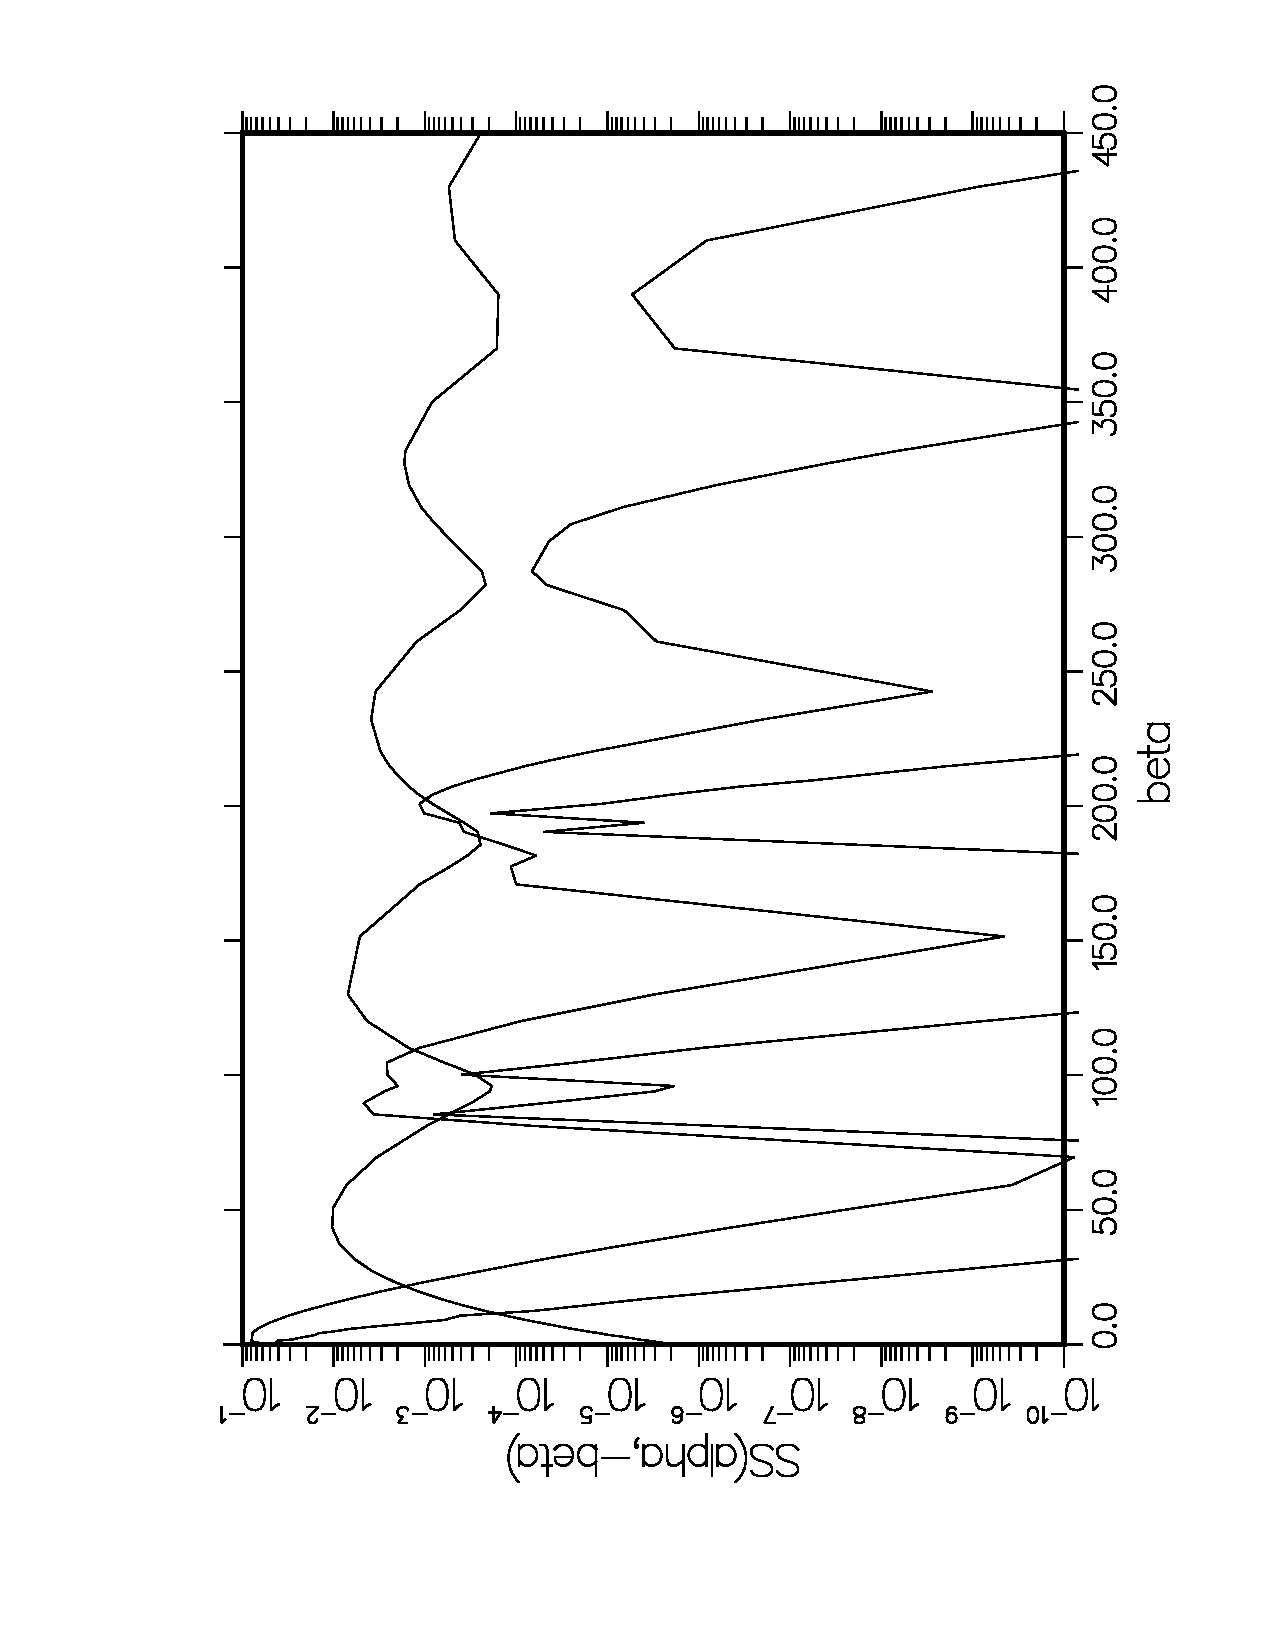
\includegraphics[keepaspectratio, height=3.4in, angle=270]{figs/le2ack}
\caption[${\cal S}(\alpha,-\beta)$ for solid methane]{${\cal S}(\alpha,-\beta)$
 for solid methane shown as a function of $\beta$ for the $\alpha$ values 0.986
 (lowest), 16.94, and 151.45 (highest).  The four discrete levels show up as
 sharp triangles in the lowest curve.}
\label{smeths}
\end{figure}

\begin{figure}[b]\centering
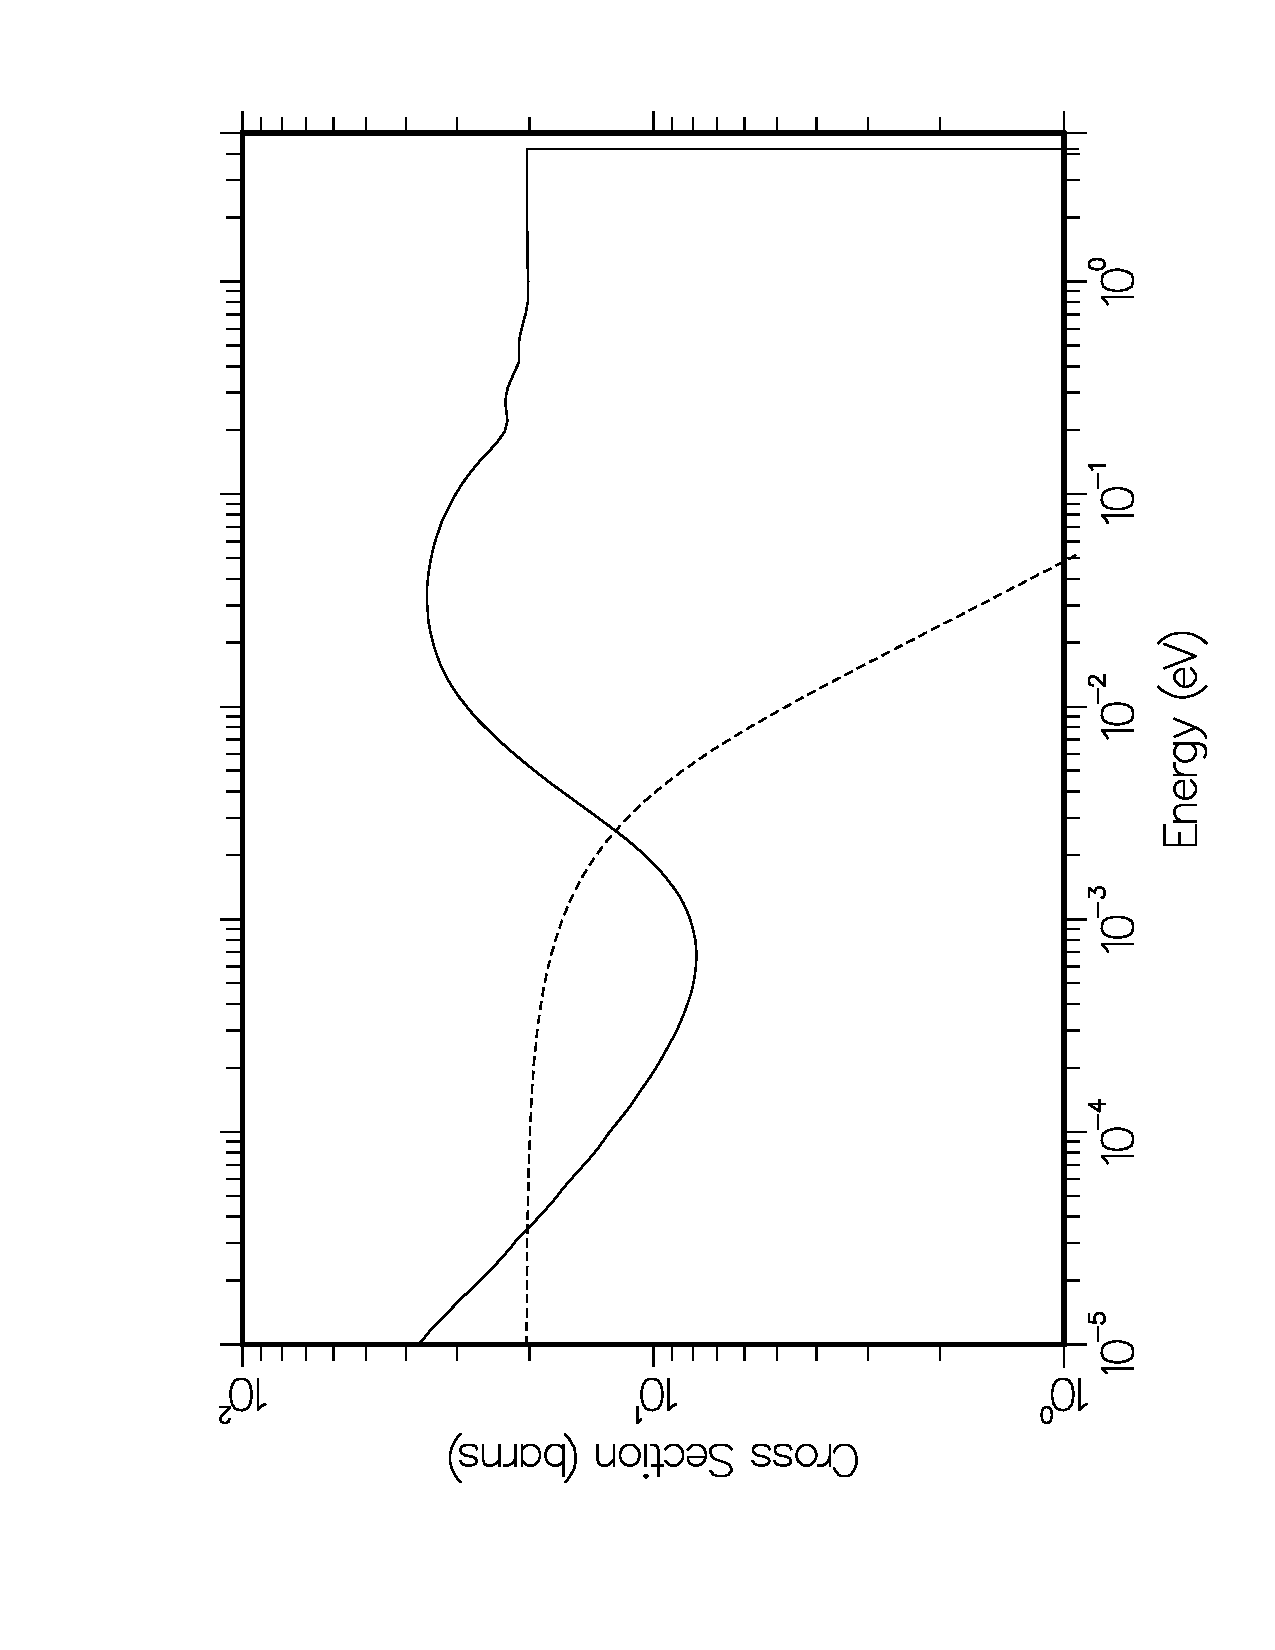
\includegraphics[keepaspectratio, height=3.4in, angle=270]{figs/le3ack}
\caption[Inelastic and incoherent elastic cross sections for solid methane]
{Inelastic (solid) and incoherent elastic (dashed) cross sections for
 solid methane.  The small bumps starting at about 0.2 eV are due to
 the discrete levels at 0.162 eV, 0.190 eV, 0.361 eV, and 0.374 eV.}
\label{smeth}
\end{figure}

Next, the new evaluation for $S(\alpha,\beta)$ can be processed into
integrated cross sections and double differential cross sections using
the \hyperlink{sTHERMRhy}{THERMR} module of NJOY.  A plot
of the integrated cross section
is given in Fig.~\ref{smeth}, and plots of the outgoing neutron
spectrum integrated over angle at several incident energies are
given in Fig.~\ref{fig4}.

\begin{figure}[t]\centering
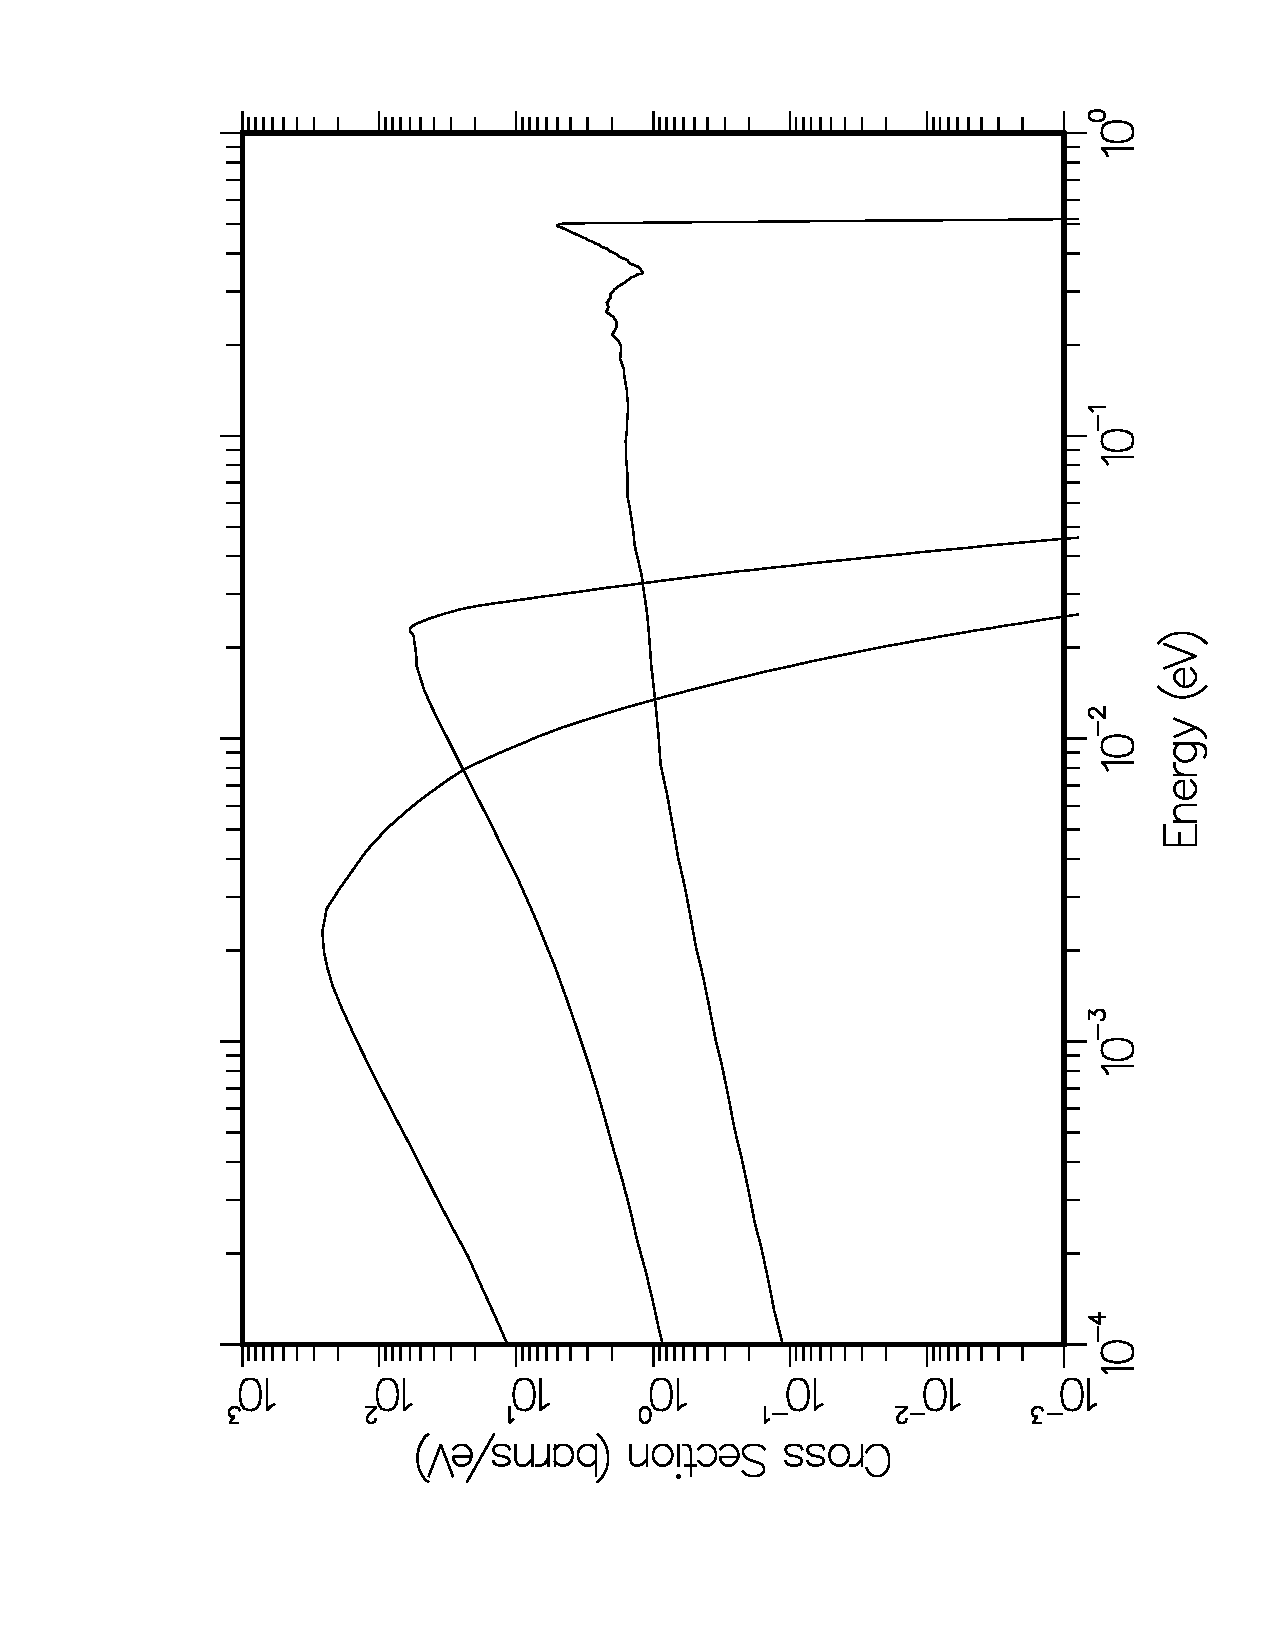
\includegraphics[keepaspectratio, height=3.4in, angle=270]{figs/le4ack}
\caption[Outgoing neutron spectra for solid methane]{Neutron spectra
 $\sigma(E{\rightarrow}E')$ for solid methane shown as functions of
 outgoing neutron energy $E'$ for $E=$0.0001 eV, 0.0253 eV, and 0.503 eV.}
\label{fig4}
\end{figure}

\paragraph{The Model for Liquid Methane.}
This example is for liquid methane at 100K.  Once again, we use the
four discrete oscillators to represent the the molecular vibrations.
 In addition, we need a continuous frequency distribution to represent
the molecular rotations, and a pair of parameters $d$ and $c$ to
represent diffusion.  This latter component was omitted from the
earlier model of Picton, but we felt that it might be needed to obtain a
reasonable quasi-elastic peak in the spectrum of scattered neutrons.
Therefore, we couldn't use the Picton input directly, and we had to refer
to his source\cite{AYY}.  Agrawal and Yip divided the problem into two
parts: translations and rotations.

For translations, they proposed a model for $\gamma(t)$ that matches the
expected diffusive behavior at long times and provides an oscillatory
behavior at short times.  Each methane molecule is assumed to move in a
``cage" formed by its neighbors, and the cage itself is allowed to
relax with time.  As Agrawal and Yip point out, the molecule will
oscillate initially, but gradually as the restoring forces decay into
a frictional background, it will go over into diffusive motions.  The
resulting analytic expression for the frequency spectrum is

\begin{equation}
   f_t(\omega)=\frac{2}{\pi}\,\frac{\omega_0^2/\tau_0}
      {(\omega^2-\omega_0^2)^2+(\omega/\tau_0)^2}\,.
   \label{liq1}
\end{equation}

\noindent
The fact that $f(\omega)$ is nonzero at $\omega{=}0$ indicates that the
molecules are capable of diffusion, and in addition, $f(\omega)$ has
a resonant behavior near $(\omega^2{-}\tau_0^2)^{1/2}$, the characteristic
frequency of local oscillations.

For rotations, the argument starts out by recalling that for translations,
$\gamma(t)$ is related to the mean-square displacement $W(t)$ by

\begin{equation}
   \gamma(t)=\kappa^2W(t)\,,
\end{equation}

\noindent
where the magnitude of the wave vector is related to $\alpha$ by

\begin{equation}
   \alpha=\frac{\hbar^2\kappa^2}{2MkT}\,.
\end{equation}

\noindent
The rotational analog of the mean-square displacement is the mean-square
component of the bond length $\vec{b}$ along the the vector $\vec{\kappa}$, or

\begin{eqnarray}
   W(t)&=&<[b_\kappa(t)-b_\kappa(0)]>^2\nonumber\\
       &=&2<b_\kappa^2>\left[1-\frac{<b_\kappa(t)
            b_\kappa(0)>}{<b_\kappa^2>}\right]\nonumber\\
       &=&\frac{2b^2}{3}\Bigl[1-F_1(t)\Bigr]\,.
\end{eqnarray}
The function $F_1(t)$  is seen to describe the correlation between a
specific direction in the molecule at $t{=}0$ with its direction at a later
time $t$.  Therefore, it is called the ``dipole correlation function''.
The same function appears in the classical limit of the theory of
optical line shapes for infrared absorption as presented by
Gordon\cite{Gordon}.  At frequencies where it is safe to assume that
the internal vibrations of different molecules are uncoupled, the shape
of a vibrational line depends mostly on the reorientation motions of
individual molecules, and the dipole correlation function can be
obtained from

\begin{equation}
   F_1(t)=\int_{\rm band}\hat{I}(\omega)\cos\omega t\,d\omega.
\end{equation}

\noindent
Gordon has used this method to compute $F_1(t)$ for liquid methane at
98K based on the infrared data of Ewing\cite{Ewing}.  In order to link this
result to neutron scattering, we use the high-temperature classical limit
of Eq.\ref{gamma} to express $W(t)$; namely,

\begin{equation}
   W(\hat{t})=\frac{\hbar^2}{2MkT}\int_0^\infty
      \frac{\rho_r}{\beta^2}\Bigl[1-\cos(\beta\hat{t})\Bigr]\,d\beta,
\end{equation}
\vspace{0.5 pt}

\noindent
which can be inverted to obtain

\begin{equation}
   \rho_r(\beta)=\frac{2MkT}{\hbar^2}\intall
       \frac{d^2\gamma_r}{dt^2}\rm e^{i\beta\hat{t}}\,d\hat{t}\,.
\end{equation}

\noindent
This limit is justified by noting that $\beta{<}1$ for the rotational modes
in liquid methane around 90K.  It is now easy to compute $\rho_r$ by taking
two derivatives of the dipole correlation function graphed by Gordon.

The result is shown in Fig.~\ref{fig5}, together with the translational
frequency distribution discussed above.  These numbers were generated by
digitizing the curve from Agrawal and Yip, subtracting the translational
part, and smoothing the remainder.  Agrawal and Yip compared their model
with both double-differential and integrated cross sections, with very good
agreement.

\begin{figure}[t]\centering
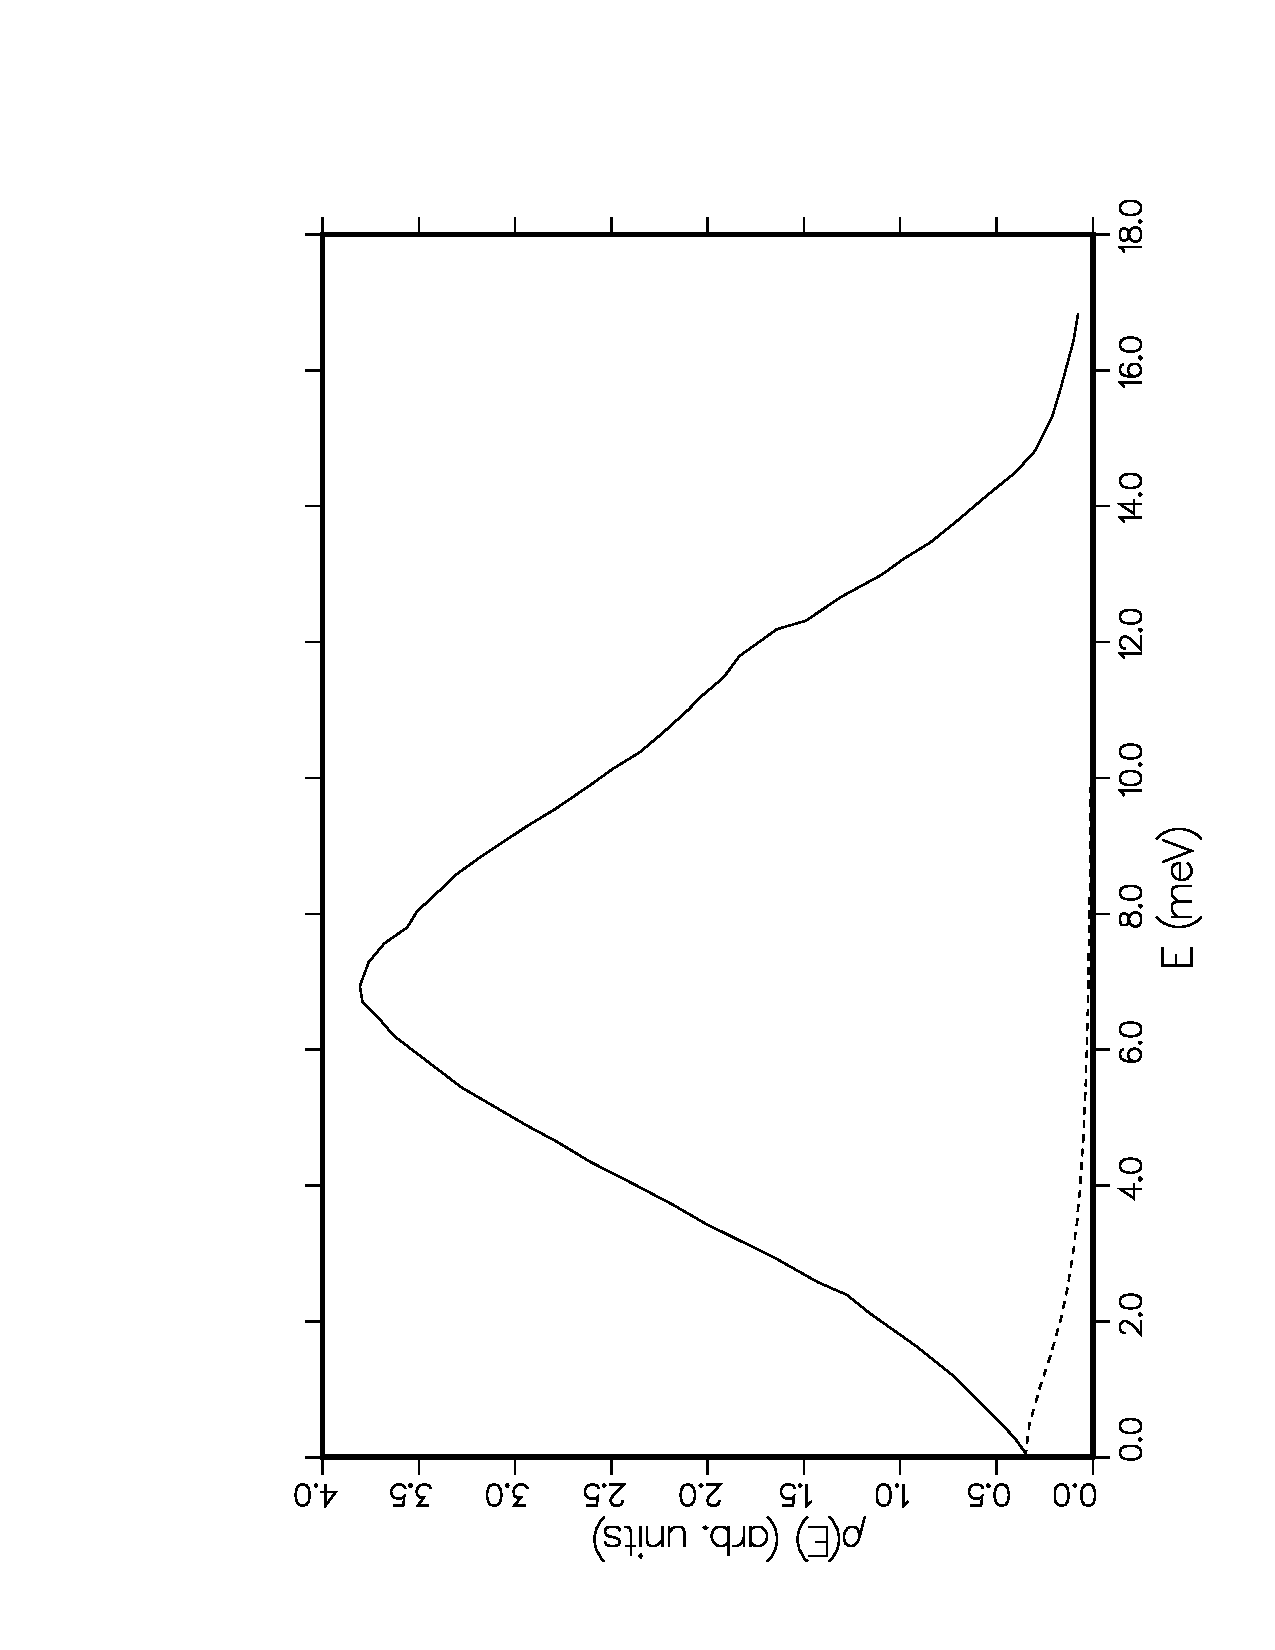
\includegraphics[keepaspectratio, height=3.4in, angle=270]{figs/le5ack}
\caption[Agrawal-Yip frequency spectrum for liquid methane]
  {Frequency spectrum for liquid methane (solid) as given by
  Agrawal and Yip, including an analytic translational part (dashed)
  and a rotational part based on Gordon's analysis
  of the optical measurements of Ewing.}
\label{fig5}
\end{figure}

\begin{figure}[b]\centering
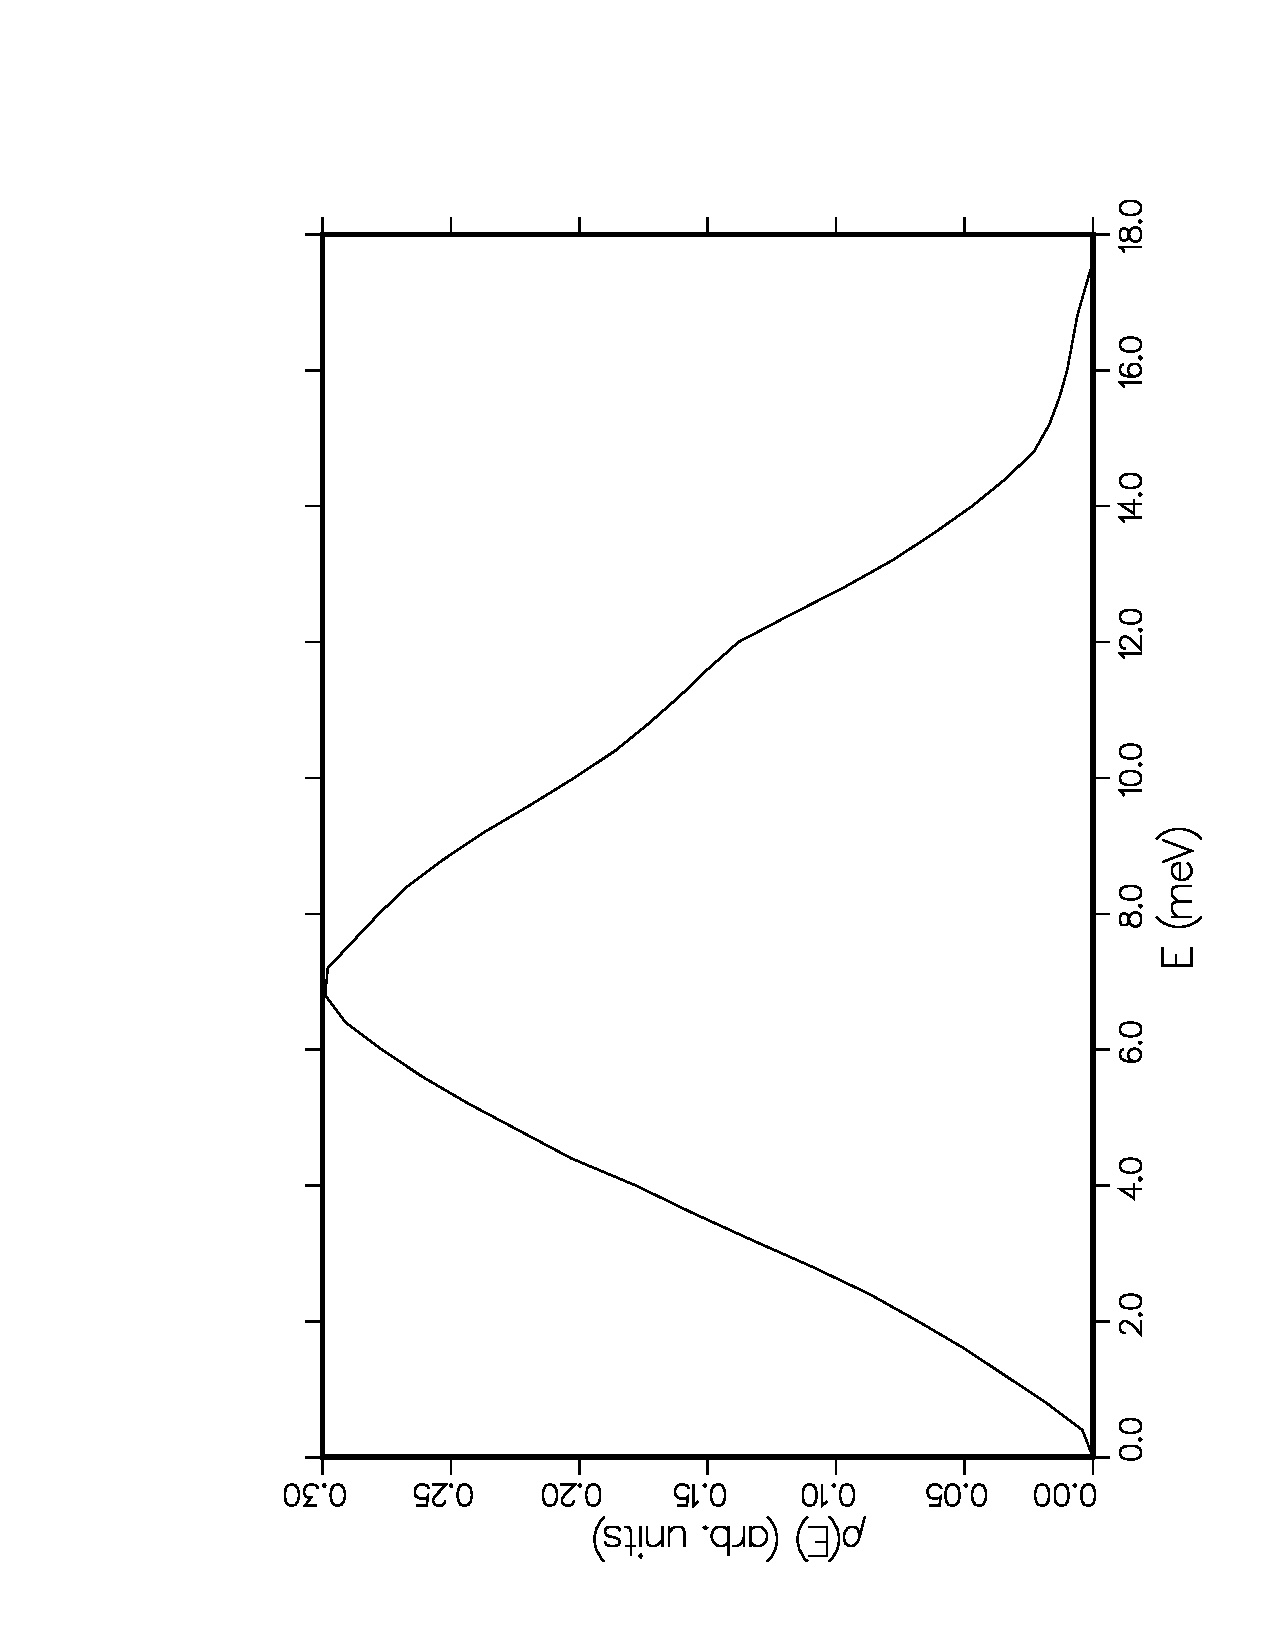
\includegraphics[keepaspectratio, height=3.4in, angle=270]{figs/le6ack}
\caption[Frequency spectrum for liquid methane with translational and
 rotational modes]{Effective frequency spectrum for methane including
 both translational and rotational modes, but not including diffusive modes.}
\label{fig6}
\end{figure}

Unfortunately, this model does not match the requirements of LEAPR.  The
only type of frequency distribution that is nonzero at $\omega{=}0$ that
can be used by the code is the diffusive law of Egelstaff and Schofield,
which does not have the short-time oscillatory behavior of Eq. \ref{liq1}.
Our main reason for using the diffusion term in our model for liquid methane
was to improve the ``quasi-elastic" peak, which depends mostly on the
small-$\omega$ part of the frequency distribution.  Therefore, it seemed
reasonable to select diffusion parameters $d$ and $c$ that gave a reasonable
representation for the full width at half maximum of the quasi-elastic
peak, to subtract the result $f_d$ from the sum of the two curves shown
in Fig.~\ref{fig5}, and to use the difference to represent both the
translational oscillatory modes and the rotational modes.  Fig.~\ref{fig6}
shows this breakdown. Once again, there has been some hand smoothing, and
the low energy part of the distribution was forced to follow an $\omega^2$
law.  The final breakdown was 1.5\% diffusion, 30.5\% rotation, and 68\%
molecular vibrations.

The LEAPR input for liquid methane at 100K is shown below.

\small
\begin{ccode}

liquid methane at 100k, modified agrawal & yip model
  89  81/
  .0387  .0775  .0902  .1032  .1159
   .1419  .1677  .1934  .2191  .2578  .3096 .3610
   .4255  .4900  .5801  .6706  .7865  .9155  1.0831
   1.2638  1.4702  1.7280  2.0116  2.3600  2.7597  3.2237
   3.7654  4.4103  5.1581  6.0221  7.0538  8.2401  9.6456
   11.2704  13.1531  15.4743  18.0534  19.3429  20.8902 22.5665
   24.5010  26.6933  28.8852  33.6566  39.4596  41.7805  45.3912
   46.0362  46.5518  47.7124  48.2218  49.0020  51.5810  53.9022
   58.0287  60.6077  62.6711  63.8314  66.2815  67.6999  69.1187
   70.9239  72.7291  73.7608  78.6611  83.5613  86.1404  90.0089
   93.2326  96.4566  98.0039  100.8408  104.4516  109.6097  117.8625
   137.8503  140.5583  144.6847  149.5850  161.1907  183.4447  208.7711
   237.5941  270.3965  307.7273  350.2124  398.5625  453.5881 516.2107/
  0.0  .0387  .0775  .0902
   .1032  .1159  .1419  .1677  .1934  .2191  .2578
   .3096  .3610  .4255  .4900  .5801  .6706  .7865
   .9155  1.0831  1.2638  1.4702  1.7280  2.0116  2.3600
   2.7598  3.2237  3.7654  4.4103  5.1581  6.0221  7.0538
   8.2401  9.6456  11.2704  13.1531  15.4743  18.0538  19.3429
   20.8902  22.5665  24.5010  26.6933  28.8852  33.6566  39.4596
   41.7805  45.3912  46.0362  46.5518  47.7124  48.2281  49.0020
   51.5810  53.9022  58.0287  60.6077  62.6711  63.8314  66.2815
   67.6999  69.1187  70.9239  72.7291  73.7608  78.6611  83.5613
   86.1404  90.0089  93.2326  96.4566  98.0039  100.8408  104.4516
   109.6097  117.8625  137.8503  140.5583  144.6847  149.5850 161.1907/
 100/
 1 1/
 .00040 45/
 0. .004 .018 .034 .050 .068 .087 .109
   .133 .156 .178 .203 .223 .243 .261 .277 .291 .299
   .298 .288 .278 .267 .253 .237 .219 .202 .186 .173
   .161 .150 .138 .118 .097 .078 .062 .047 .034 .023
   .017 .013 .010 .008 .006 .003 0./
 3. 200. 0 0 .32/
 4/
  .162 .190 .361 .374/
  .308 .186 .042 .144/
 0/
 10 1001. 1.008 20.3 1 0 8/
' L-CH4     LANL       EVAL-FEB88 MACFARLANE'/
' NO REF TO DATE       DIST-'/
'----ENDF/B-6          MATERIAL'/
'-----THERMAL DATA'/
'------ENDF-6'/
' LIQUID METHANE AT 100k, MODEL OF AGRAWAL AND YIP'/
' AS IMPLEMENTED BY D.J.PICTON,'/
'  MODIFIED TO INCLUDE A DIFFUSIVE COMPONENT.'/
/

\end{ccode}
\normalsize

\begin{figure}[b]\centering
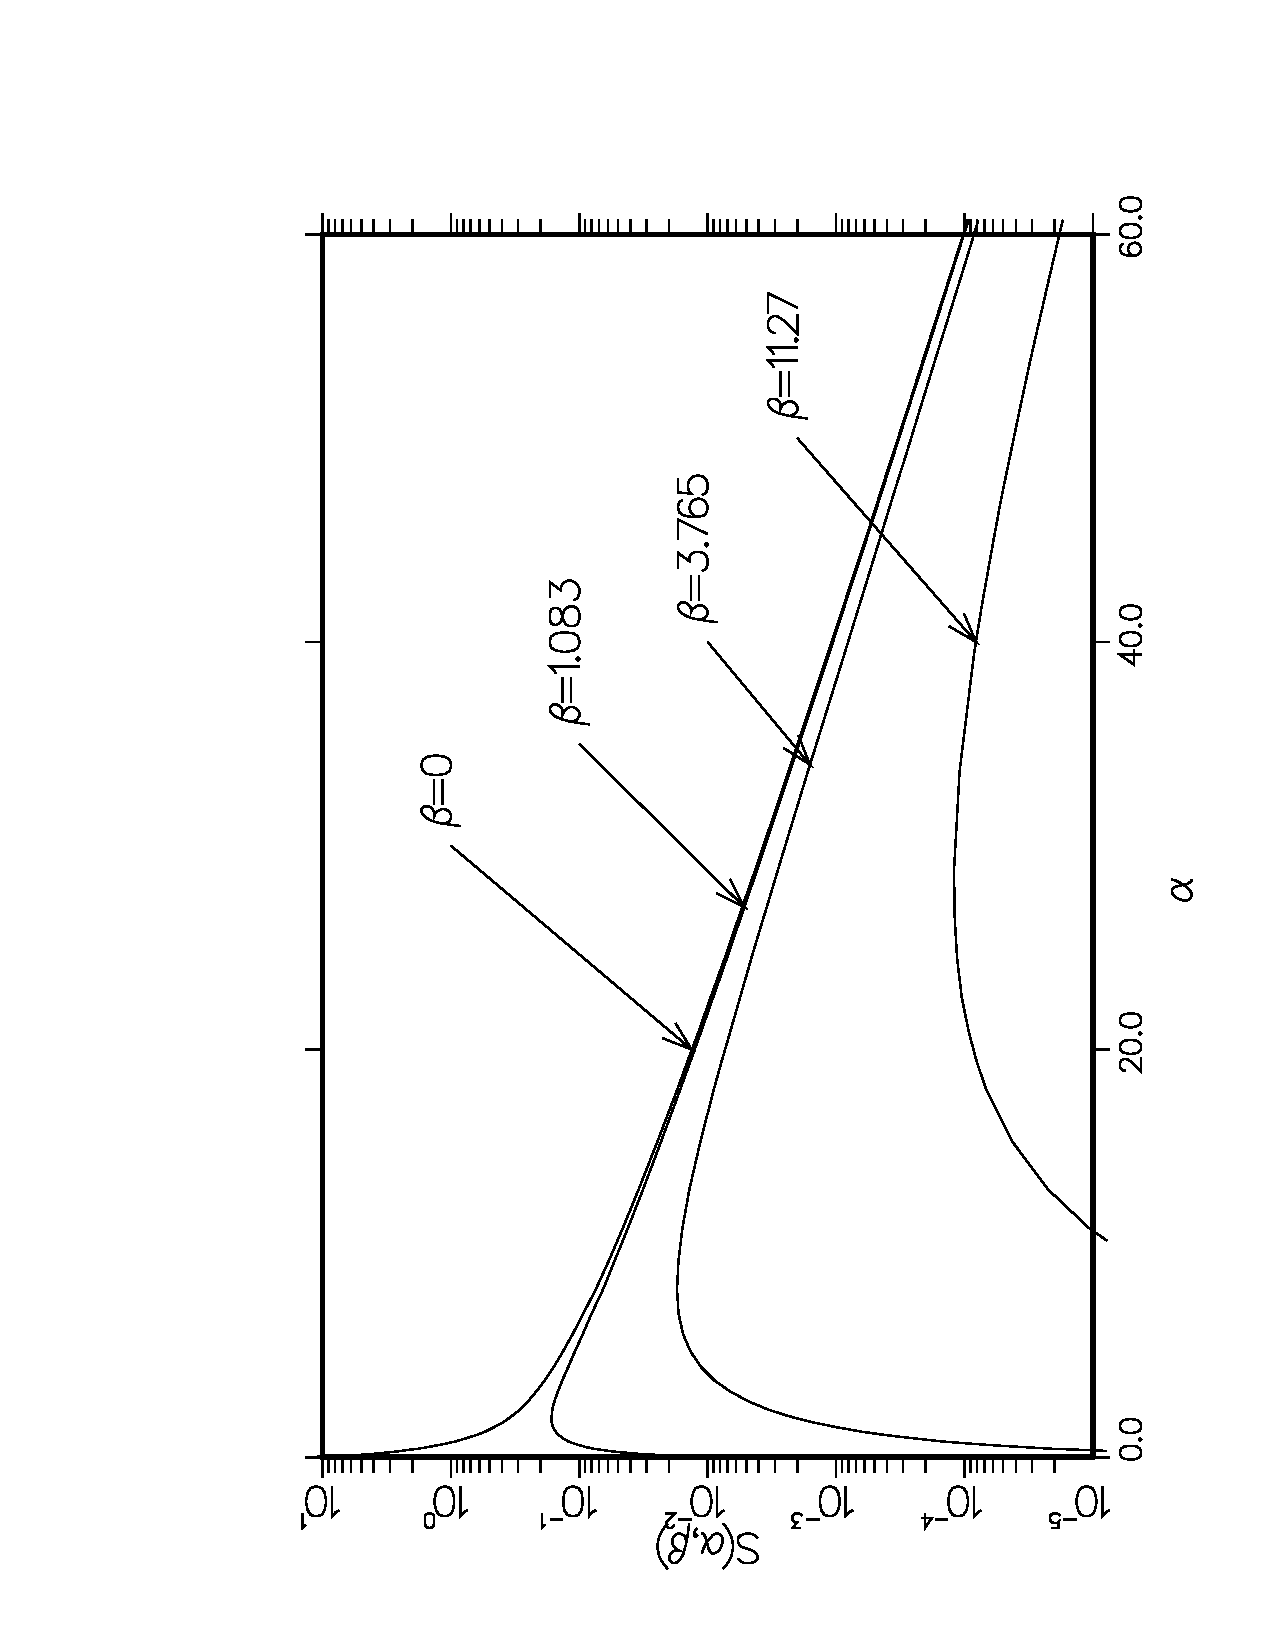
\includegraphics[keepaspectratio, height=3.5in, angle=270]{figs/le7ack}
\caption[$S(\alpha,\beta)$ for Liquid Methane]{$S(\alpha,\beta)$ curves
 for liquid methane.  Note the diffusive behavior at low $\alpha$ and $\beta$.}
\label{fig7}
\end{figure}

LEAPR can be run with this input deck.  Once again the moments of $T_n$
and $S(\beta)$ can be checked, and no great problems should be seen.  These
checks help to prove that the $\epsilon$ grid for the input frequency
spectrum and the $\beta$ grid for calculating $S$ are reasonable.  The
user should also check the range of $\alpha$ and $\beta$ to be sure that no
significant cross section contributions were being cut off. The results
should be good for all energy transfers possible with incident neutron
energies up to 1 eV. Once again, LEAPR produces an output file in
ENDF-6 format.  This time, there will be no elastic contribution at all.
Plots of $S(\alpha,\beta)$ versus $\alpha$ for several values of $\beta$
with this mode are shown in Fig.~\ref{fig7}.  Note that the behavior of
the curves for small  $\beta$ is quite different than in
Fig.~\ref{smeths}.  This reflects the presence of the diffusive component.

The new evaluation for liquid methane can be run through the
\hyperlink{sTHERMRhy}{THERMR} module
of NJOY to produce integrated and differential cross sections.  Sample
results are given in Figs.~\ref{fig8} and \ref{fig9}.  The integrated
cross section at 100K is compared with experimental data at 110K that was
quoted in the Agrawal and Yip paper.

\begin{figure}[t]\centering
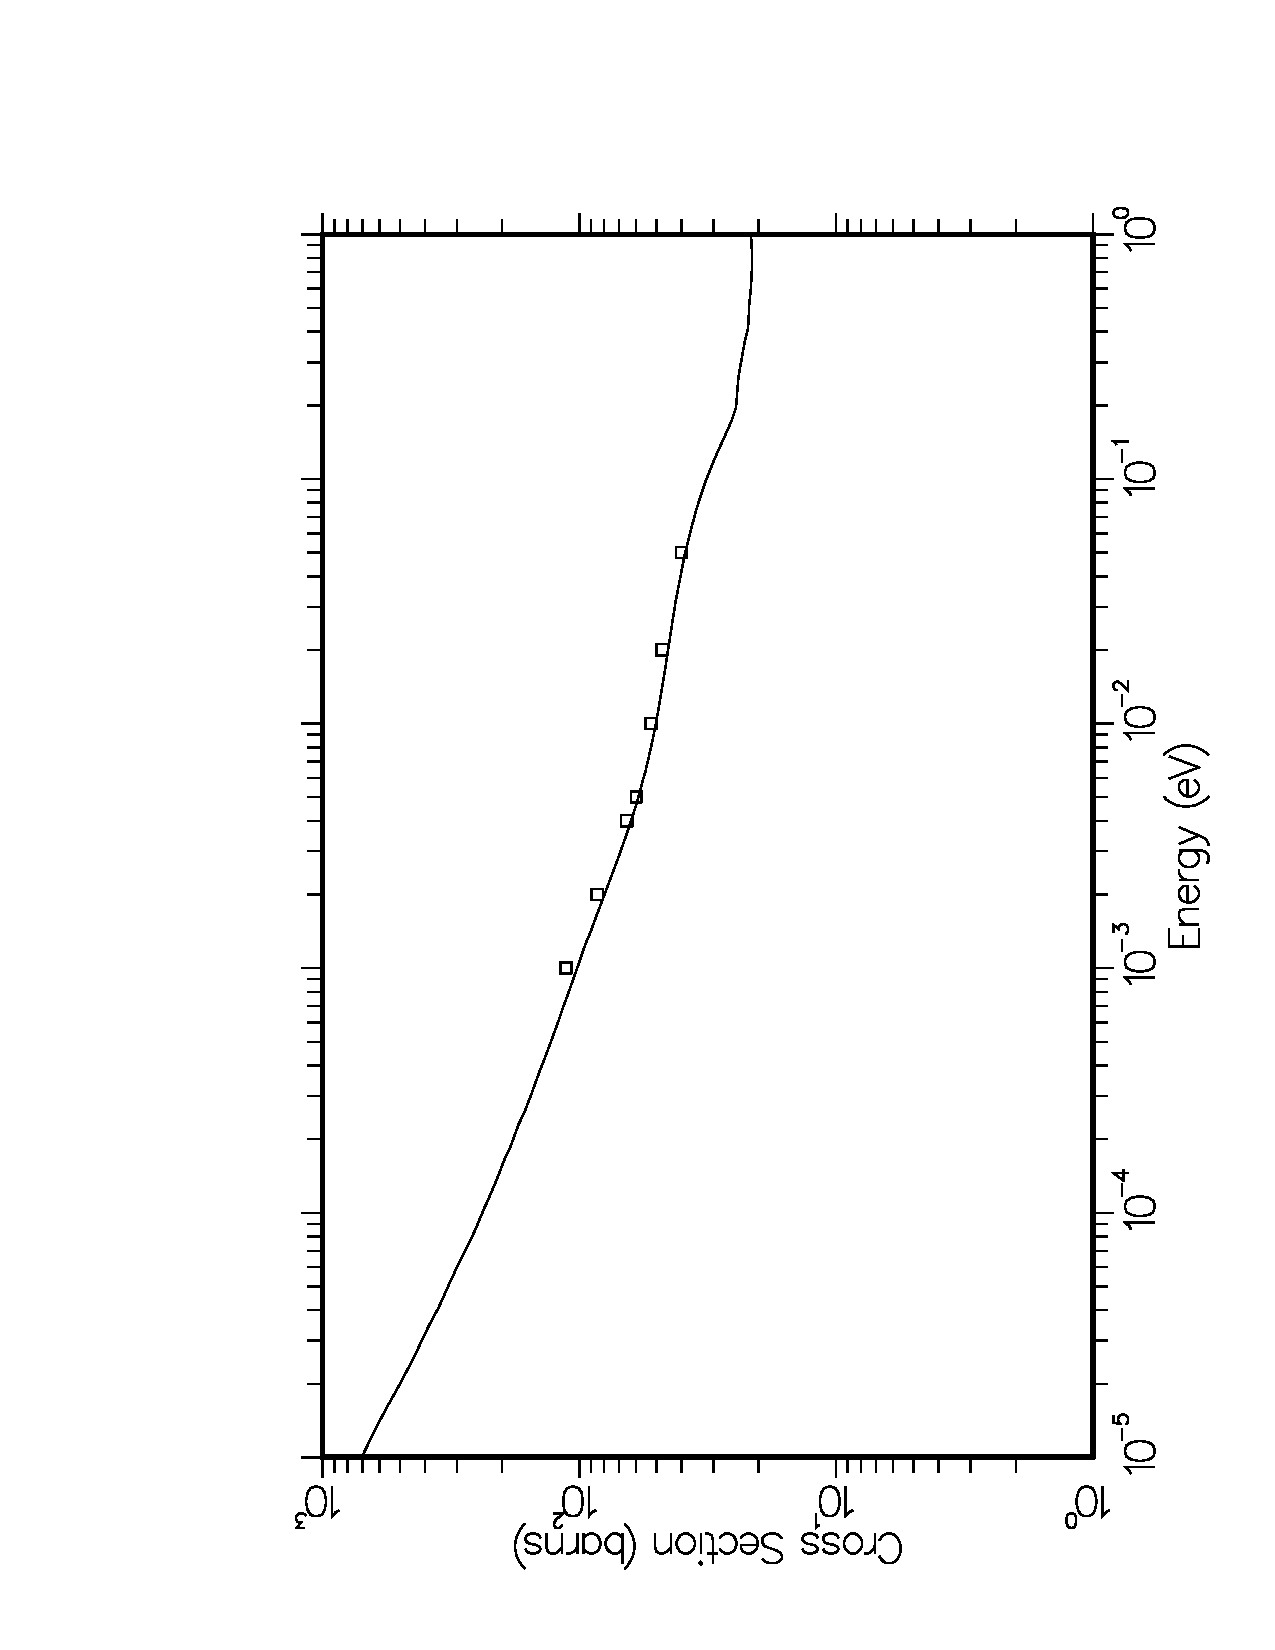
\includegraphics[keepaspectratio, height=3.5in, angle=270]{figs/le8ack}
\caption[Cross section for liquid methane at 100K]{The computed cross
 section for liquid methane at 100K (solid) is compared to experimental data
 at 110K (squares) by Whittemore and by Rogalska as quoted by Agrawal
 and Yip.}
\label{fig8}
\end{figure}

\begin{figure}[b]\centering
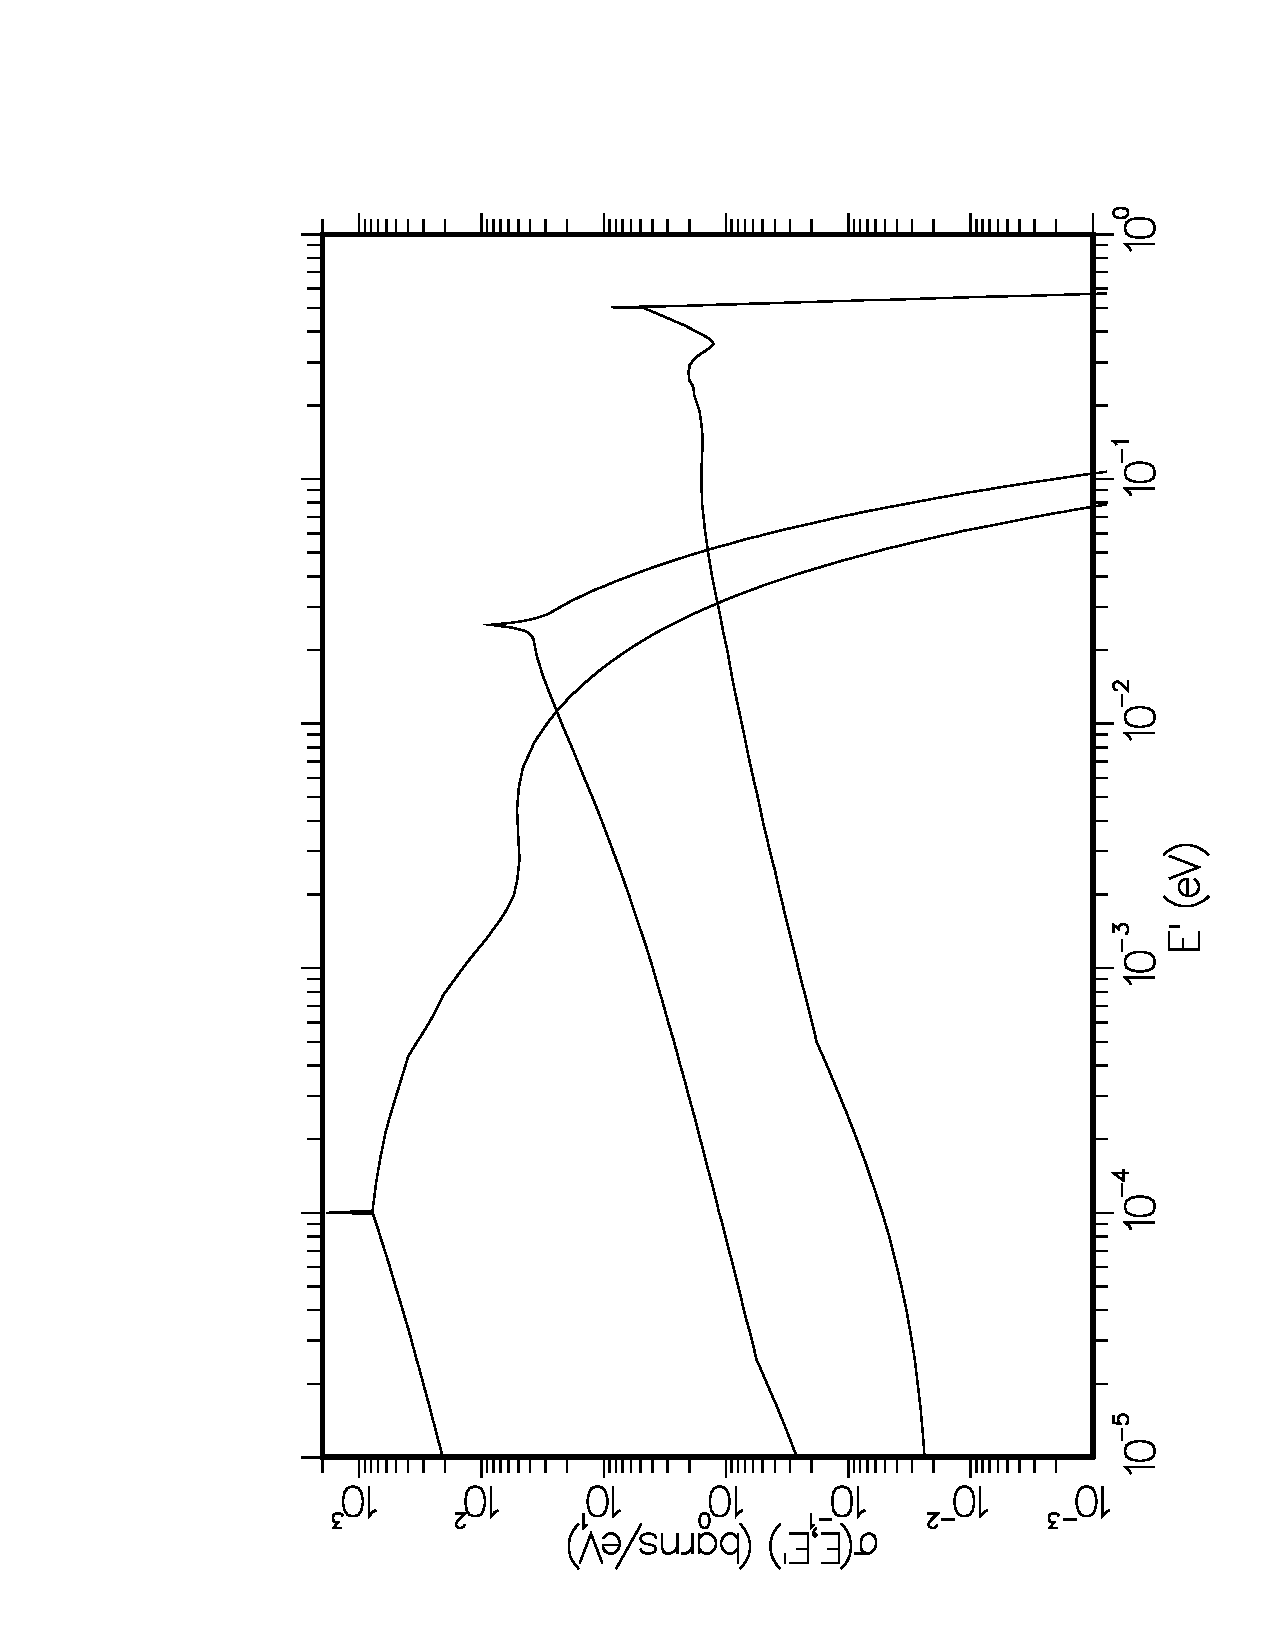
\includegraphics[keepaspectratio, height=3.5in, angle=270]{figs/le9ack}
\caption[Neutron Spectra for liquid methane]{Neutron spectra
 $\sigma(E{\rightarrow}E')$ are shown for $E=$ 0.0001 eV, 0.0253 eV, and 0.503
 eV.  Note the sharp quasi-elastic peak that results from the diffusive
 term in the theory used here.}
\label{fig9}
\end{figure}

\paragraph{The Model for Liquid Hydrogen.}
As discussed above, we picture a hydrogen molecule bound in a cluster of
about 20 molecules and undergoing vibrations similar to those of a
hydrogen molecule in a solid.  These clumps then diffuse through the
liquid (hindered translations) according to the Egelstaff-Schofield
effective width model.  This physical situation is described by the
Keinert-Sax distribution function shown in Fig.~\ref{fig10}.  They
assumed a weight of 0.025 for the hindered translation, leaving a value
of 0.475 for the solid-like distribution.  In addition,
intermolecular coherence is taken into accound using the
Vineyard\index{Vineyard} approximation.  The static
structure factor $S(\kappa)$ was
provided by Keinert and Sax. See Fig.~\ref{skh}.

This model can then be used in LEAPR.  Some results for the
effective translational ${\cal S}(\alpha,\beta)$ to be used in
the Young and Koppel formulas are shown in Figs.~\ref{fig11a}
and \ref{fig11b}.  Because  of the spin correlations,
$S(\alpha,\beta) {\ne} S(\alpha,-\beta)$, and it is necessary to
calculate both sides of the function.  Similar results for ortho
hydrogen are shown in Figs.~\ref{fig12a} and \ref{fig12b}.
These results were then passed to the ENDF output subroutine,
which allows for asymmetric scattering functions through the
parameter ``LASYM'' in the ENDF File 7 format (it is in the
``L1'' position of the head card for MF=7, MT=4).  When LASYM=1,
the $\beta$ grid in File 7 starts with $-\beta_{\rm max}$ and
increases through zero to $+\beta_{\rm max}$.  Some examples
of energy distributions for this asymmetric case computed by
\hyperlink{sTHERMRhy}{THERMR} are shown in Figs.~\ref{fig13}
and \ref{fig14}.

A comparison of the computed cross section for para and ortho
hydrogen with experiment is shown in Fig.~\ref{fig15}.

\begin{figure}[bp]\centering
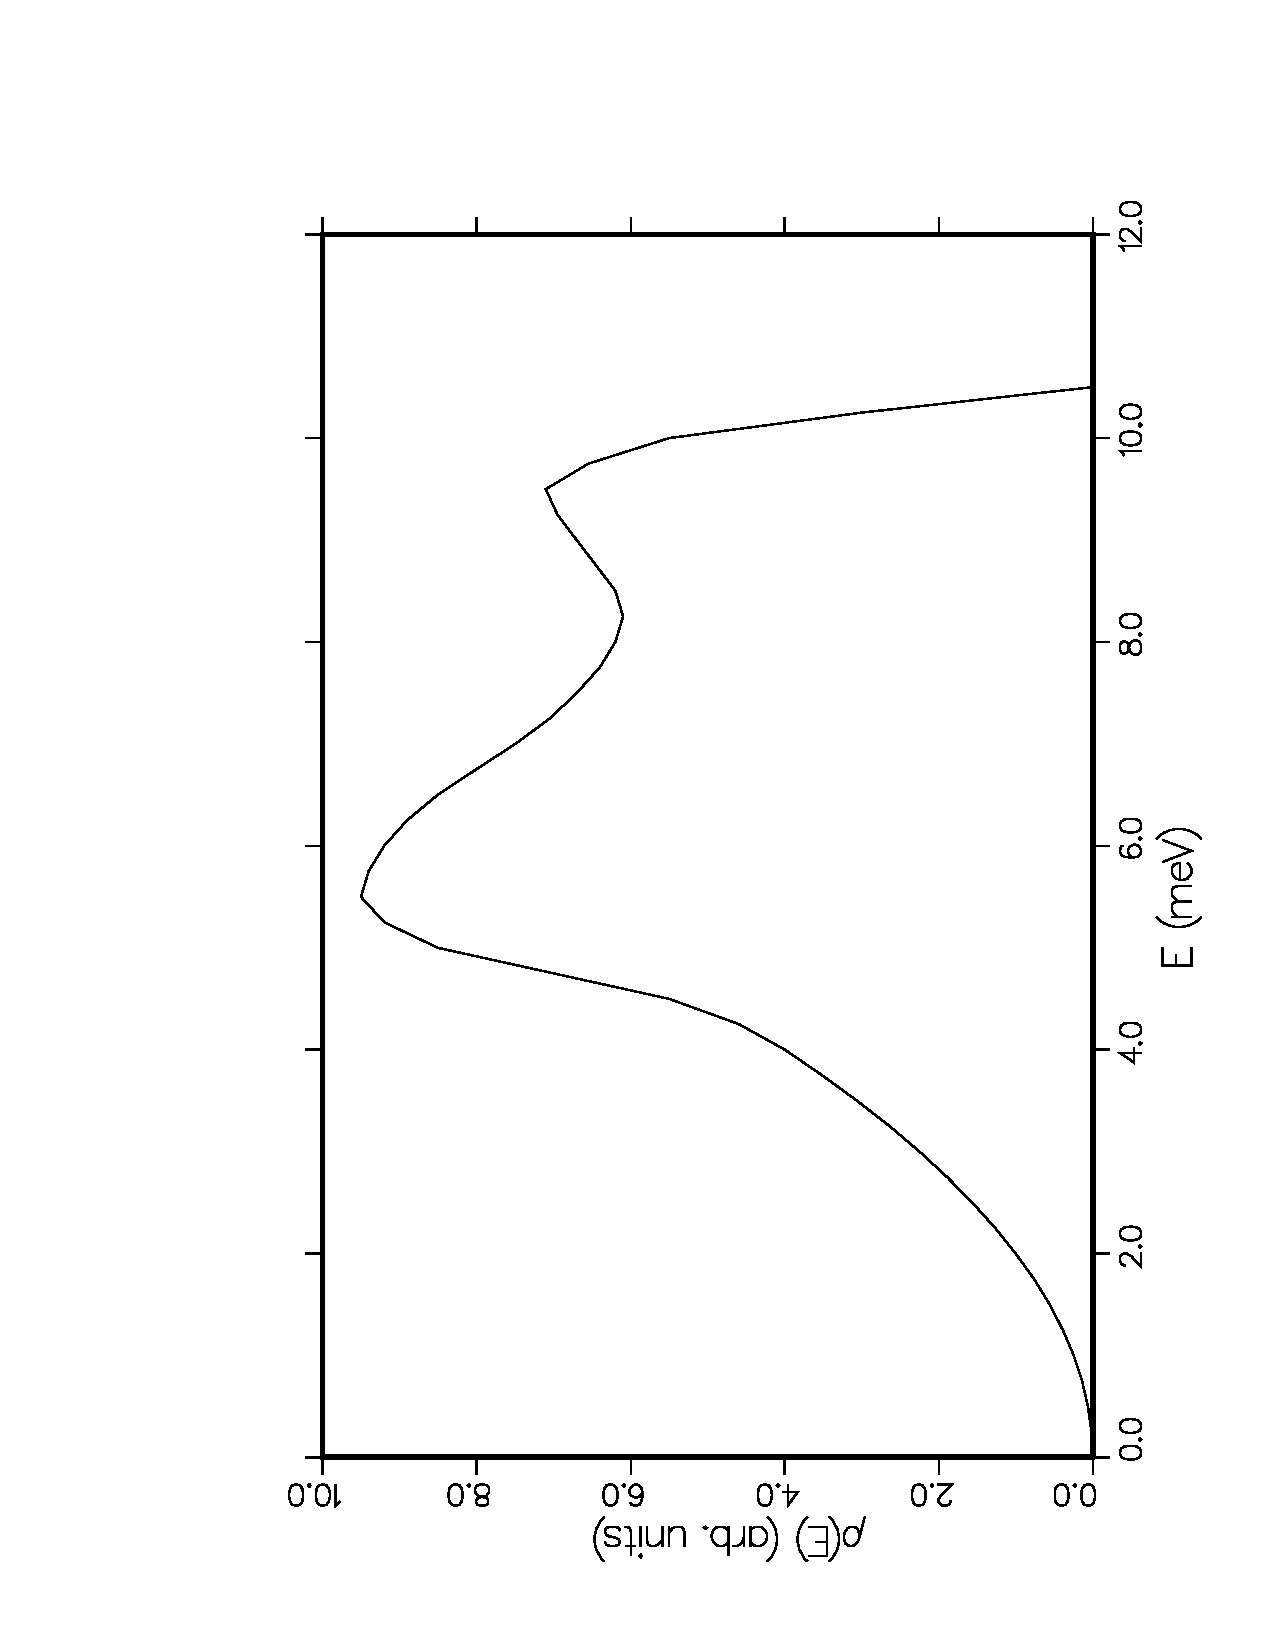
\includegraphics[keepaspectratio, height=3.7in, angle=270]{figs/le10ack}
\caption[Keinert-Sax frequency spectrum]{The Keinert-Sax frequency
 distribution for the effective translational modes of liquid hydrogen.}
\label{fig10}
\end{figure}

\begin{figure}[tp]\centering
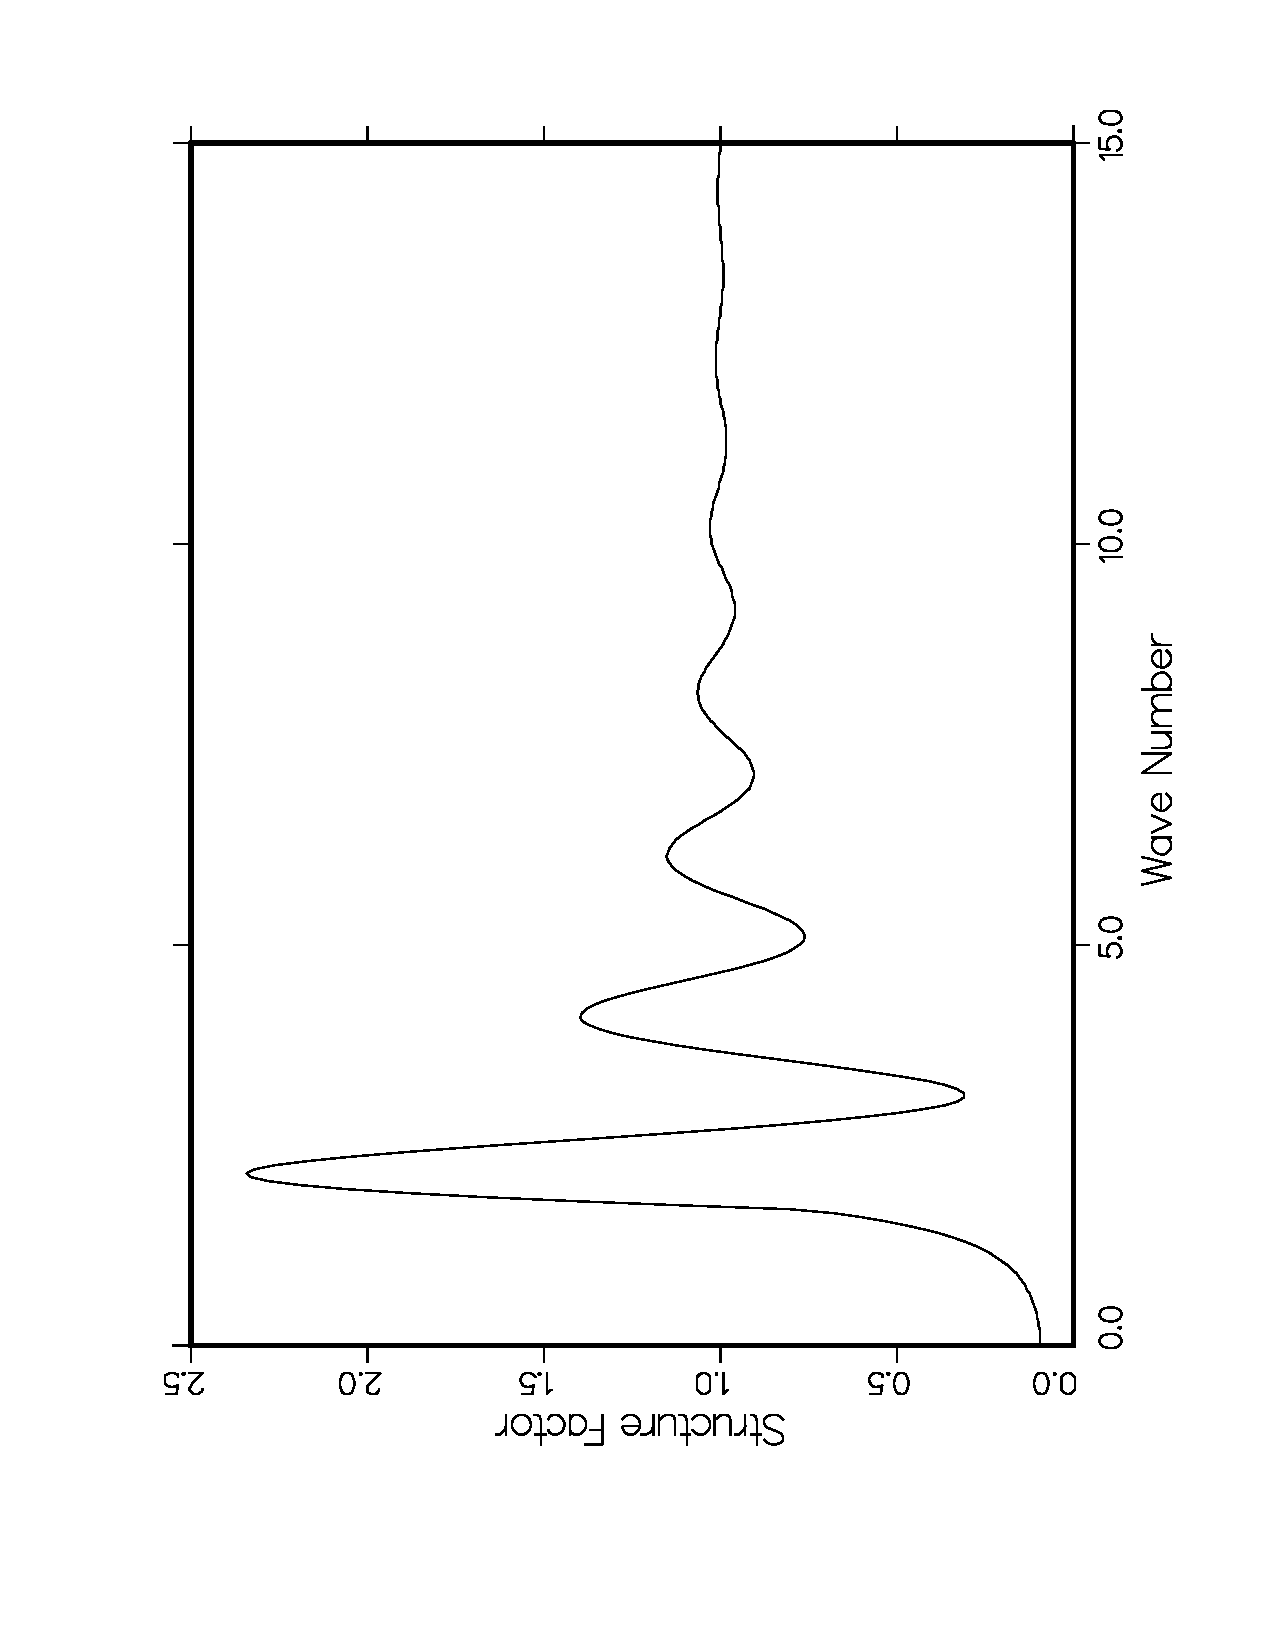
\includegraphics[keepaspectratio, height=4.0in, angle=270]{figs/le10skack}
\caption[The static structure factor, $S(\kappa)$, for liquid hydrogen]{The
 static structure factor $S(\kappa)$ for liquid hydrogen.}
\label{skh}
\end{figure}

\begin{figure}[bp]\centering
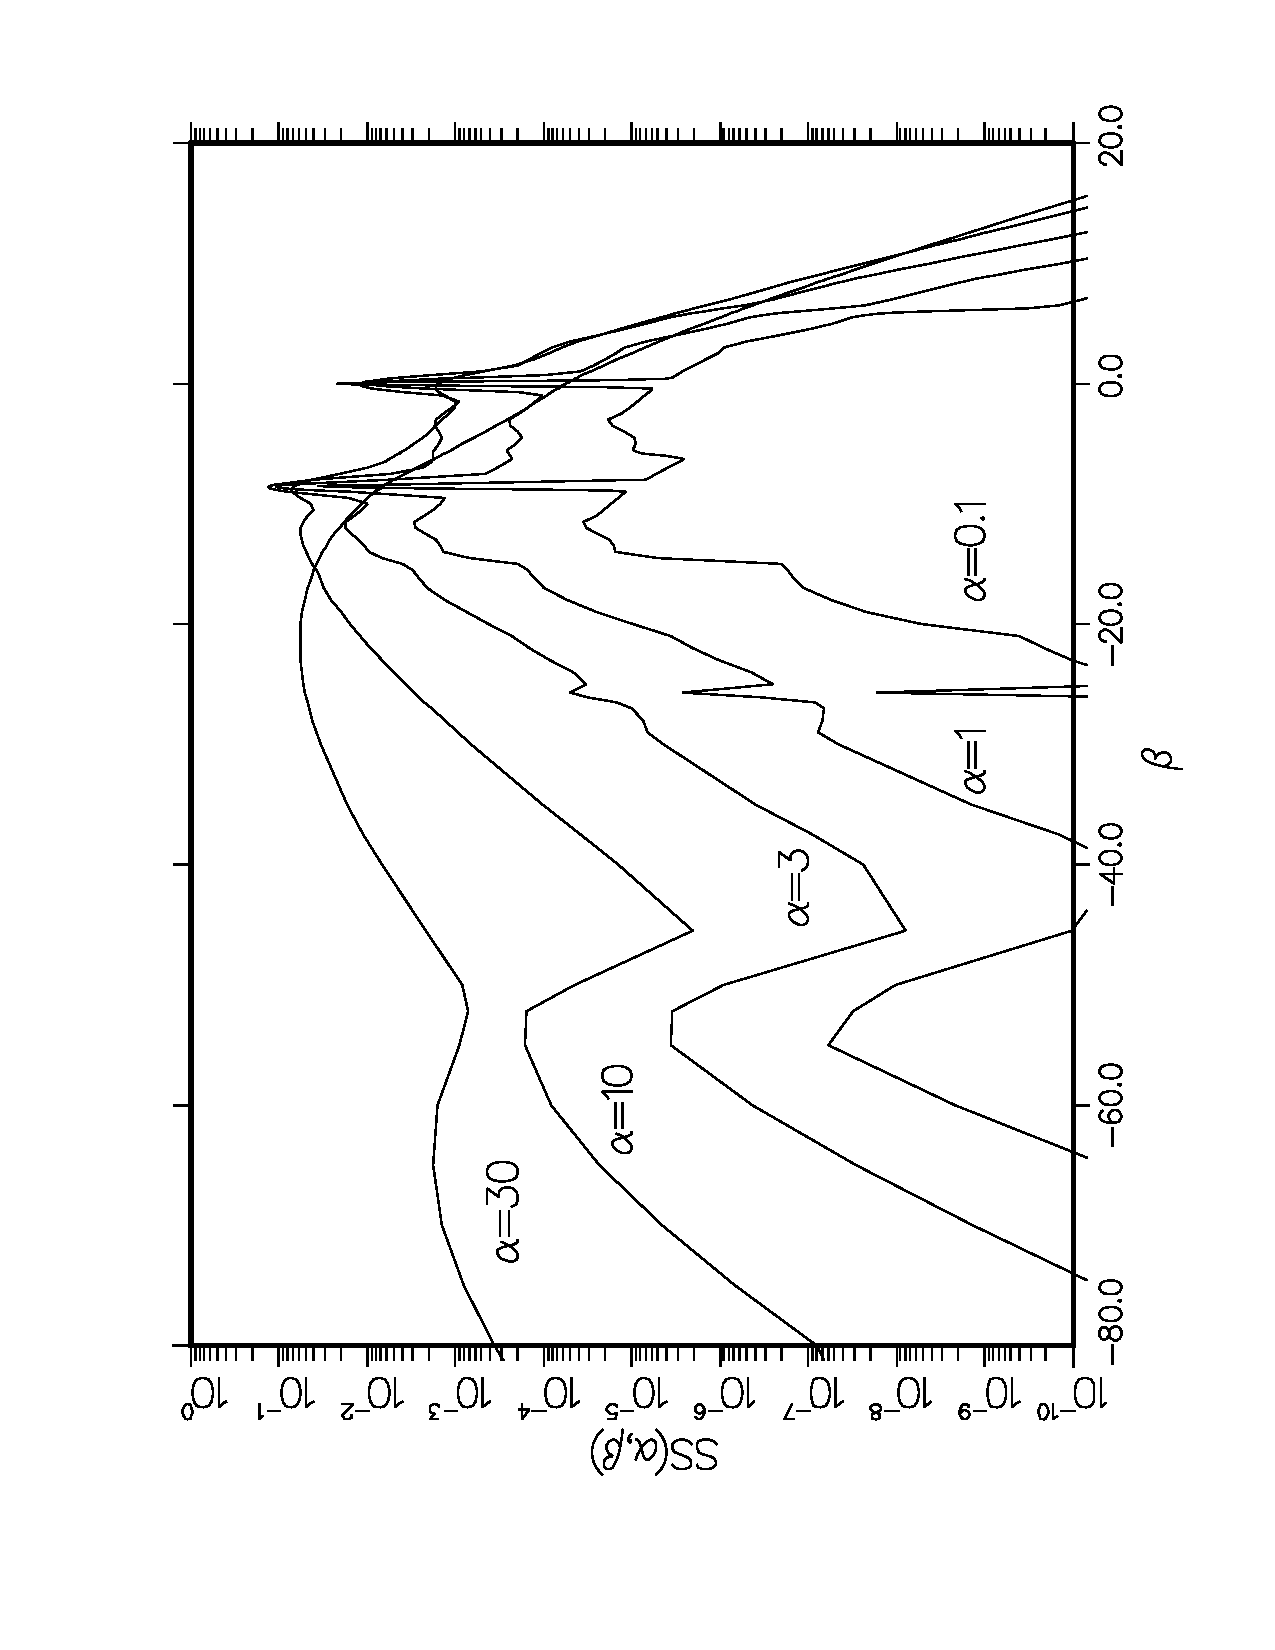
\includegraphics[keepaspectratio, height=4.0in, angle=270]{figs/le11aack}
\caption[script-S vs beta for para-hydrogen]{Script-S for para-hydrogen
 at 20K is shown as a function of $\beta$ for several $\alpha$ values.}
\label{fig11a}
\end{figure}

\begin{figure}[tp]\centering
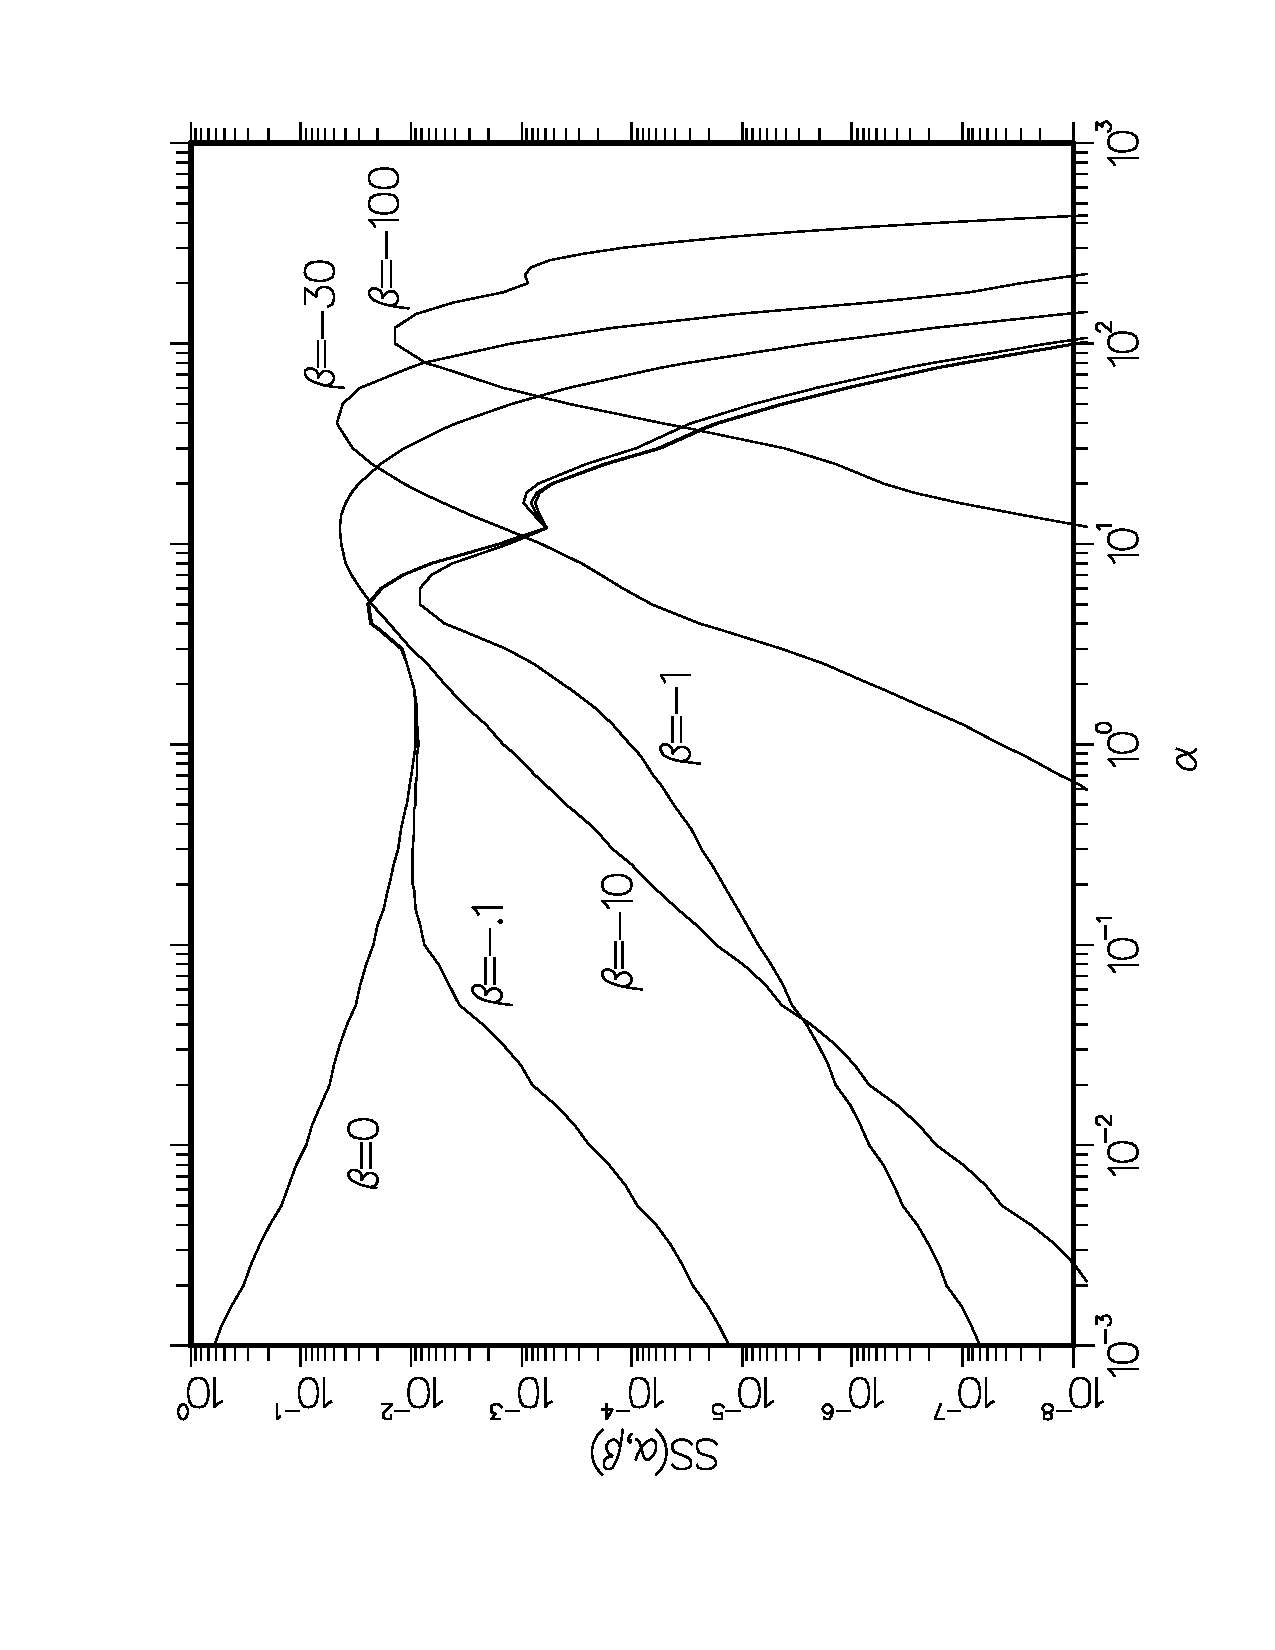
\includegraphics[keepaspectratio, height=4.0in, angle=270]{figs/le11back}
\caption[script-S vs alpha for para-hydrogen]{Script-S for para-hydrogen
 at 20K is shown as a function of $\alpha$ for several $\beta$ values
 corresponding to downscatter.}
\label{fig11b}
\end{figure}

\begin{figure}[bp]\centering
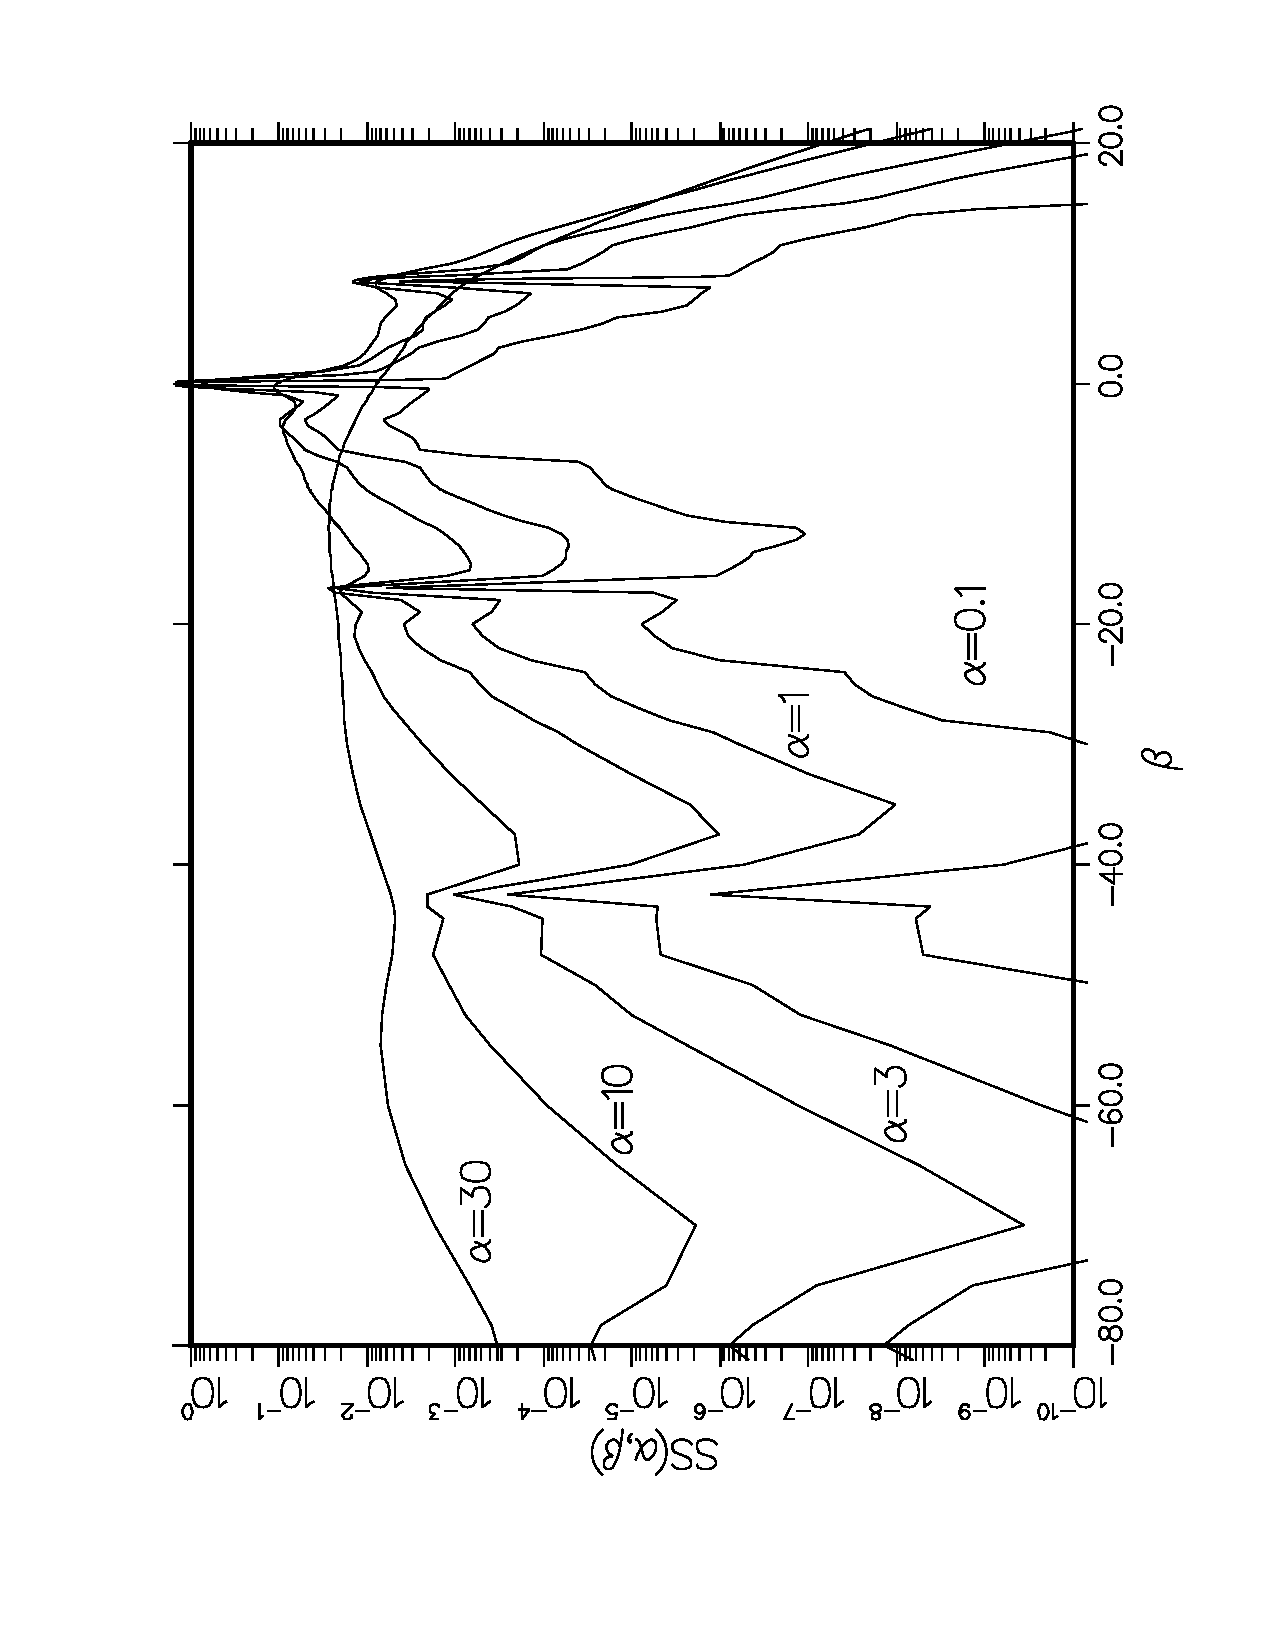
\includegraphics[keepaspectratio, height=4.0in, angle=270]{figs/le12aack}
\caption[script-S vs beta for ortho-hydrogen]{Script-S for ortho-hydrogen at
 20K is shown as a function of $\beta$ for several $\alpha$ values.}
\label{fig12a}
\end{figure}

\begin{figure}[tp]\centering
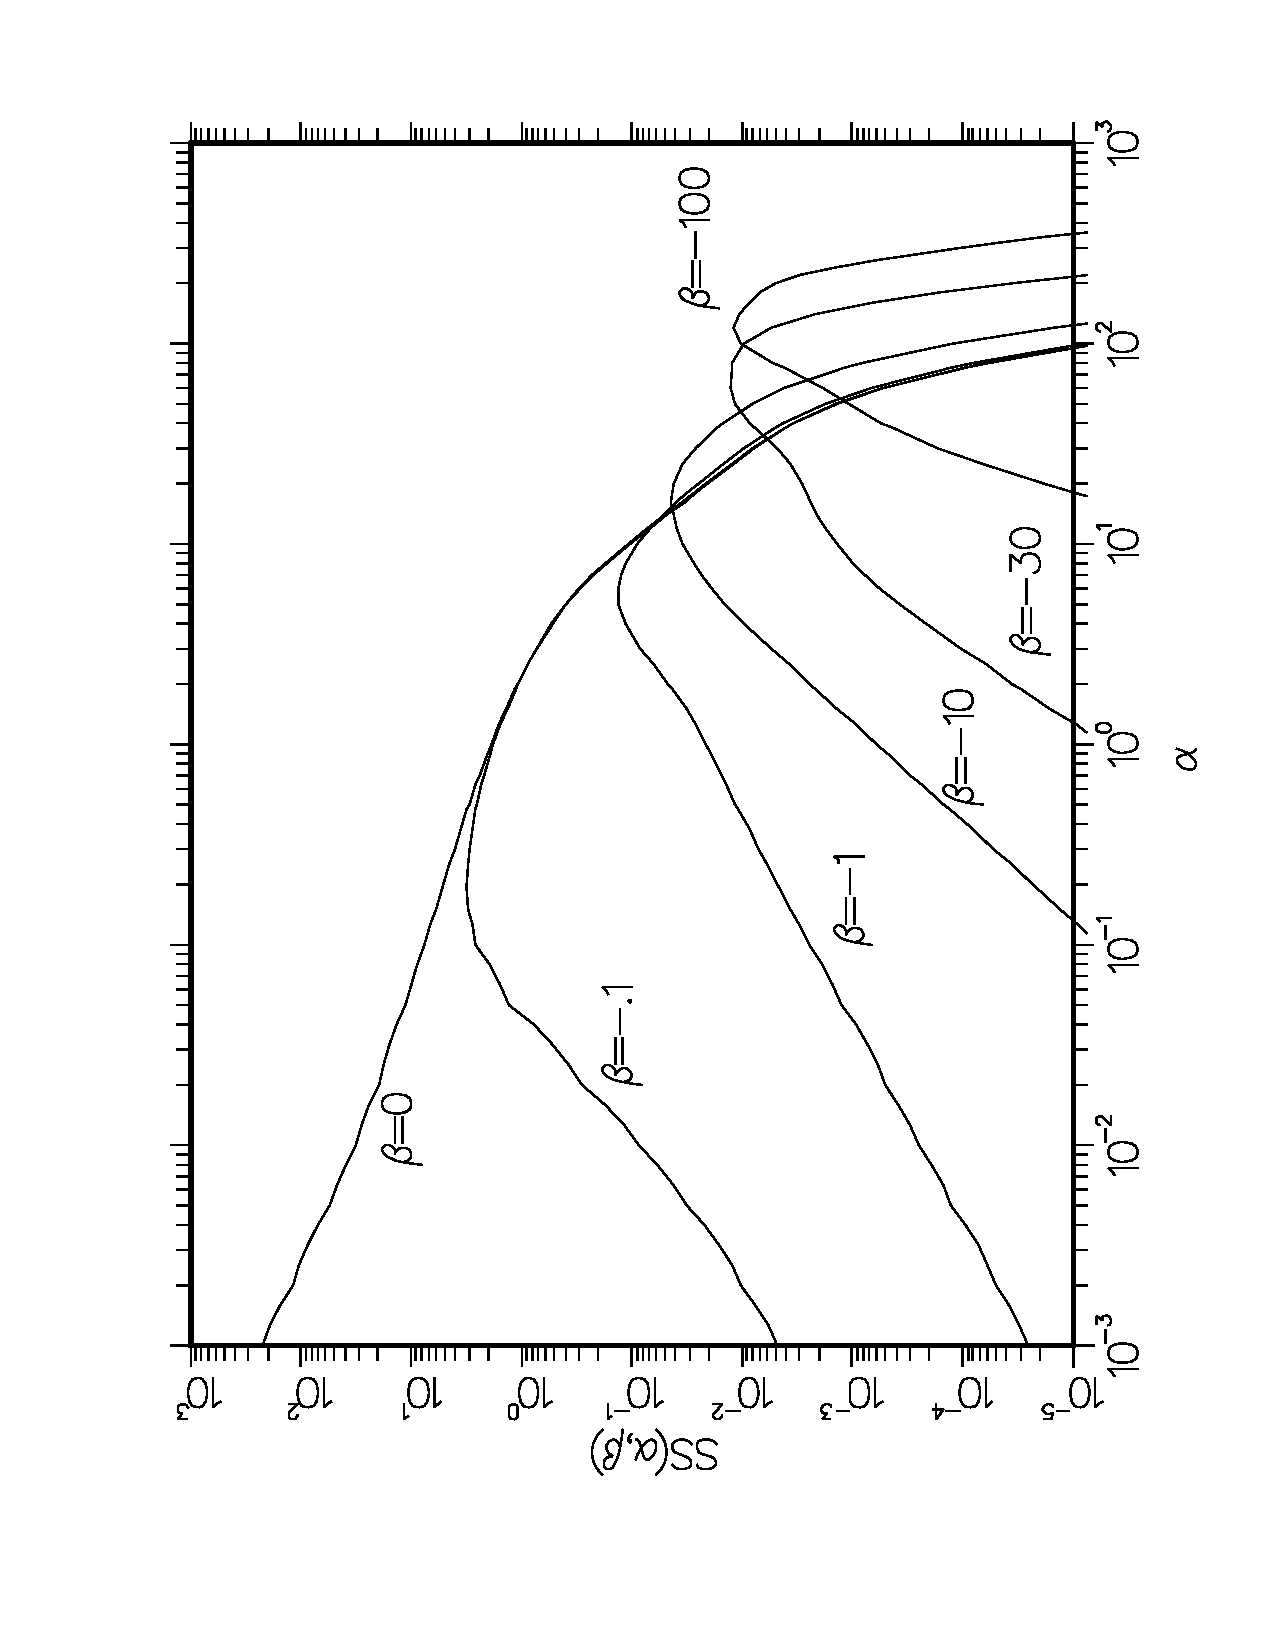
\includegraphics[keepaspectratio, height=4.0in, angle=270]{figs/le12back}
\caption[script-S vs alpha for ortho-hydrogen]{Script-S for ortho-hydrogen at
 20K is shown as a function of $\alpha$ for several $\beta$ values
 corresponding to downscatter.}
\label{fig12b}
\end{figure}

\begin{figure}[tp]\centering
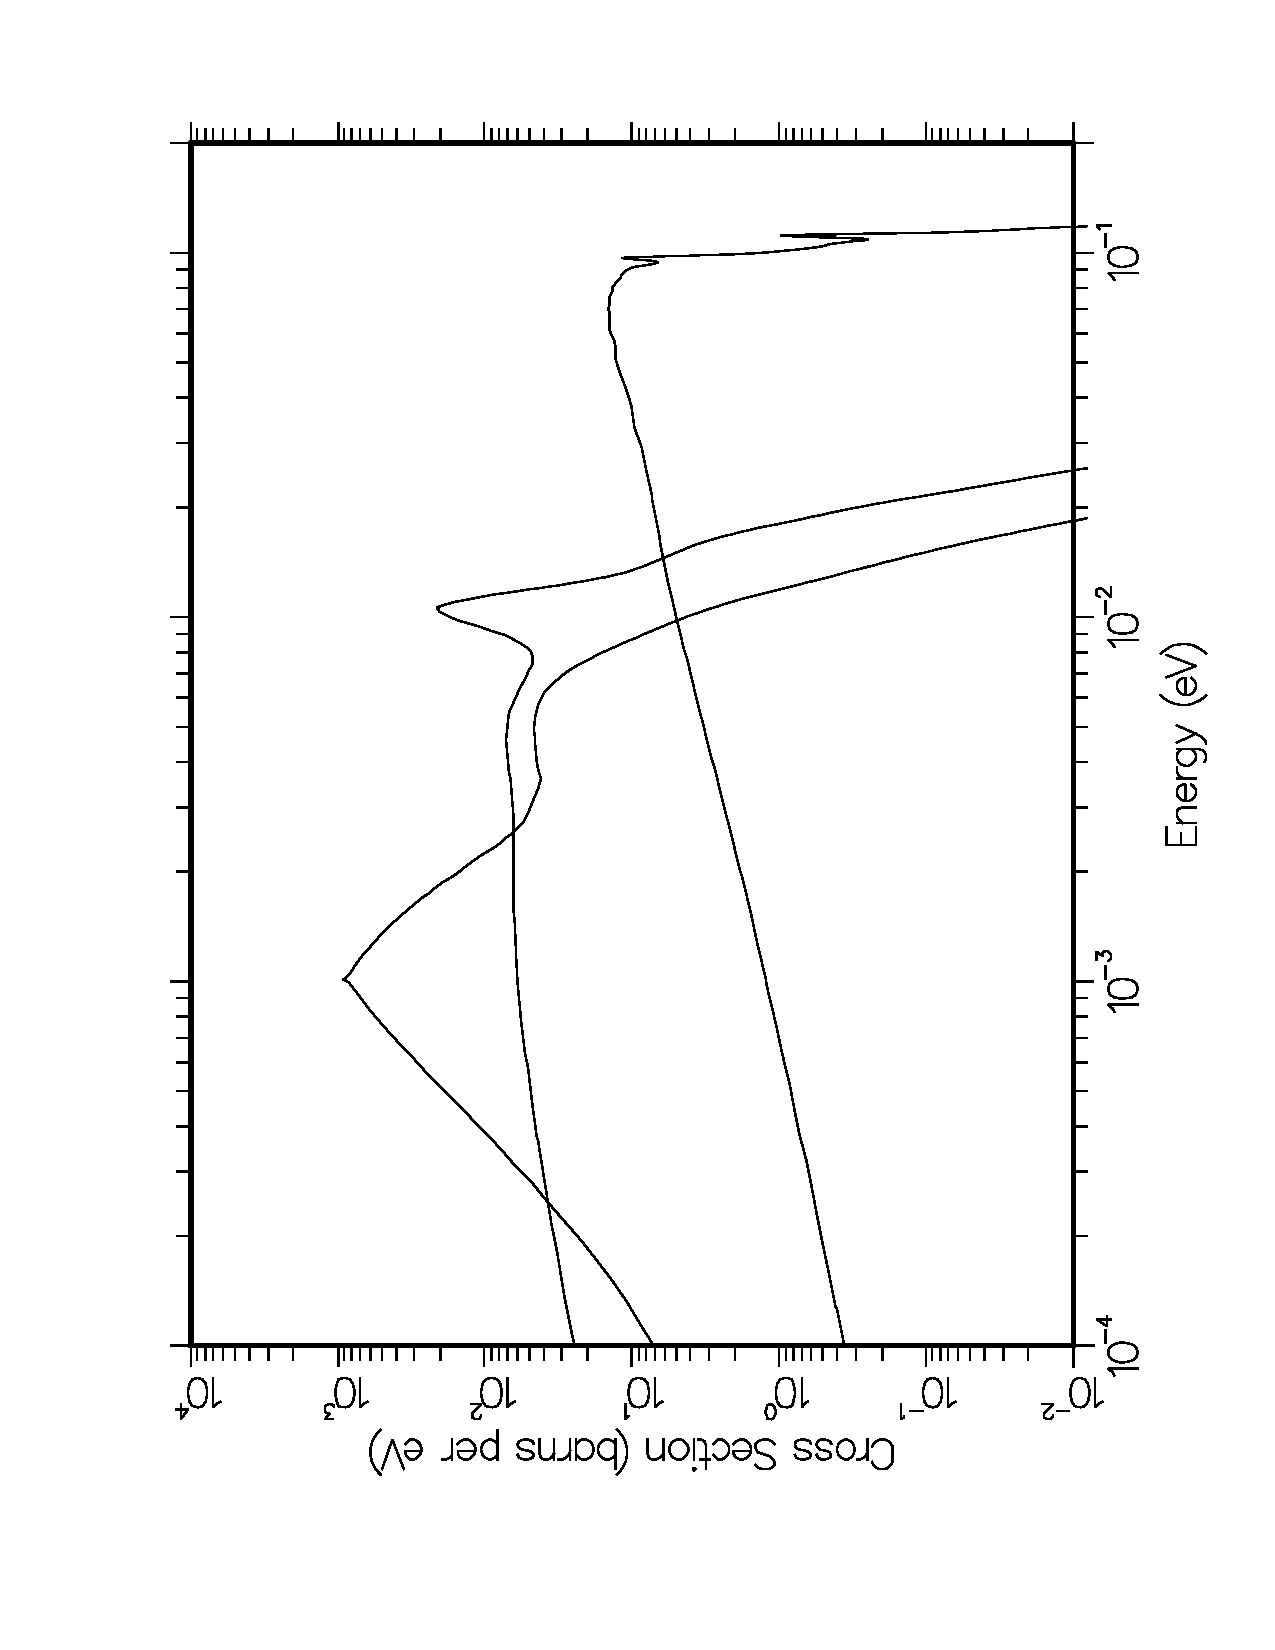
\includegraphics[keepaspectratio, height=4.0in, angle=270]{figs/le13ack}
\caption[Para-hydrogen neutron spectra]{The spectra
 $\sigma(E{\rightarrow}E')$ for liquid para-hydrogen are
 shown for $E{=}$ 0.0001 eV, 0.0106 eV, and 0.112 eV.}
\label{fig13}
\end{figure}

\begin{figure}[bp]\centering
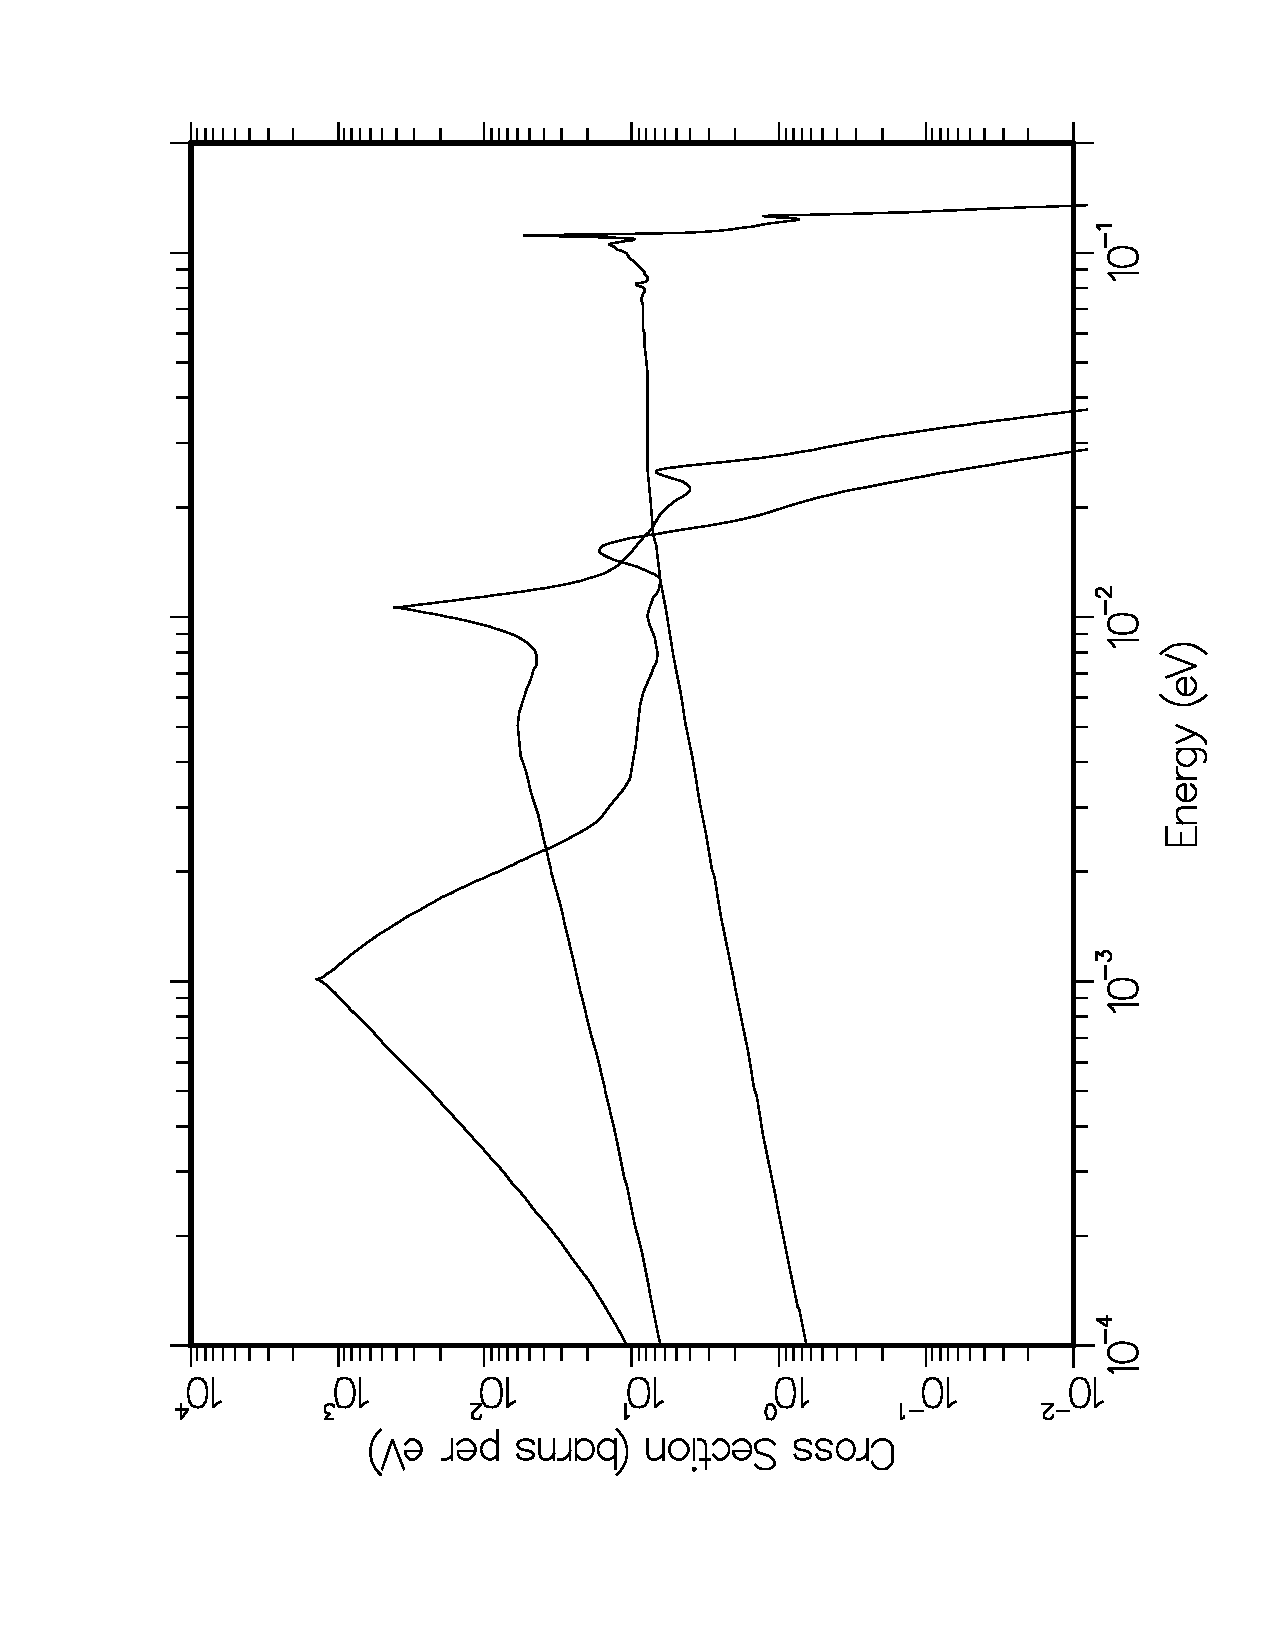
\includegraphics[keepaspectratio, height=3.8in, angle=270]{figs/le14ack}
\caption[Ortho-hydrogen neutron spectra]{The spectra
 $\sigma(E{\rightarrow}E')$ for liquid ortho-hydrogen are
 shown for $E{=}$ 0.0001 eV, 0.0106 eV, and 0.112 eV.}
\label{fig14}
\end{figure}

\begin{figure}[tp]\centering
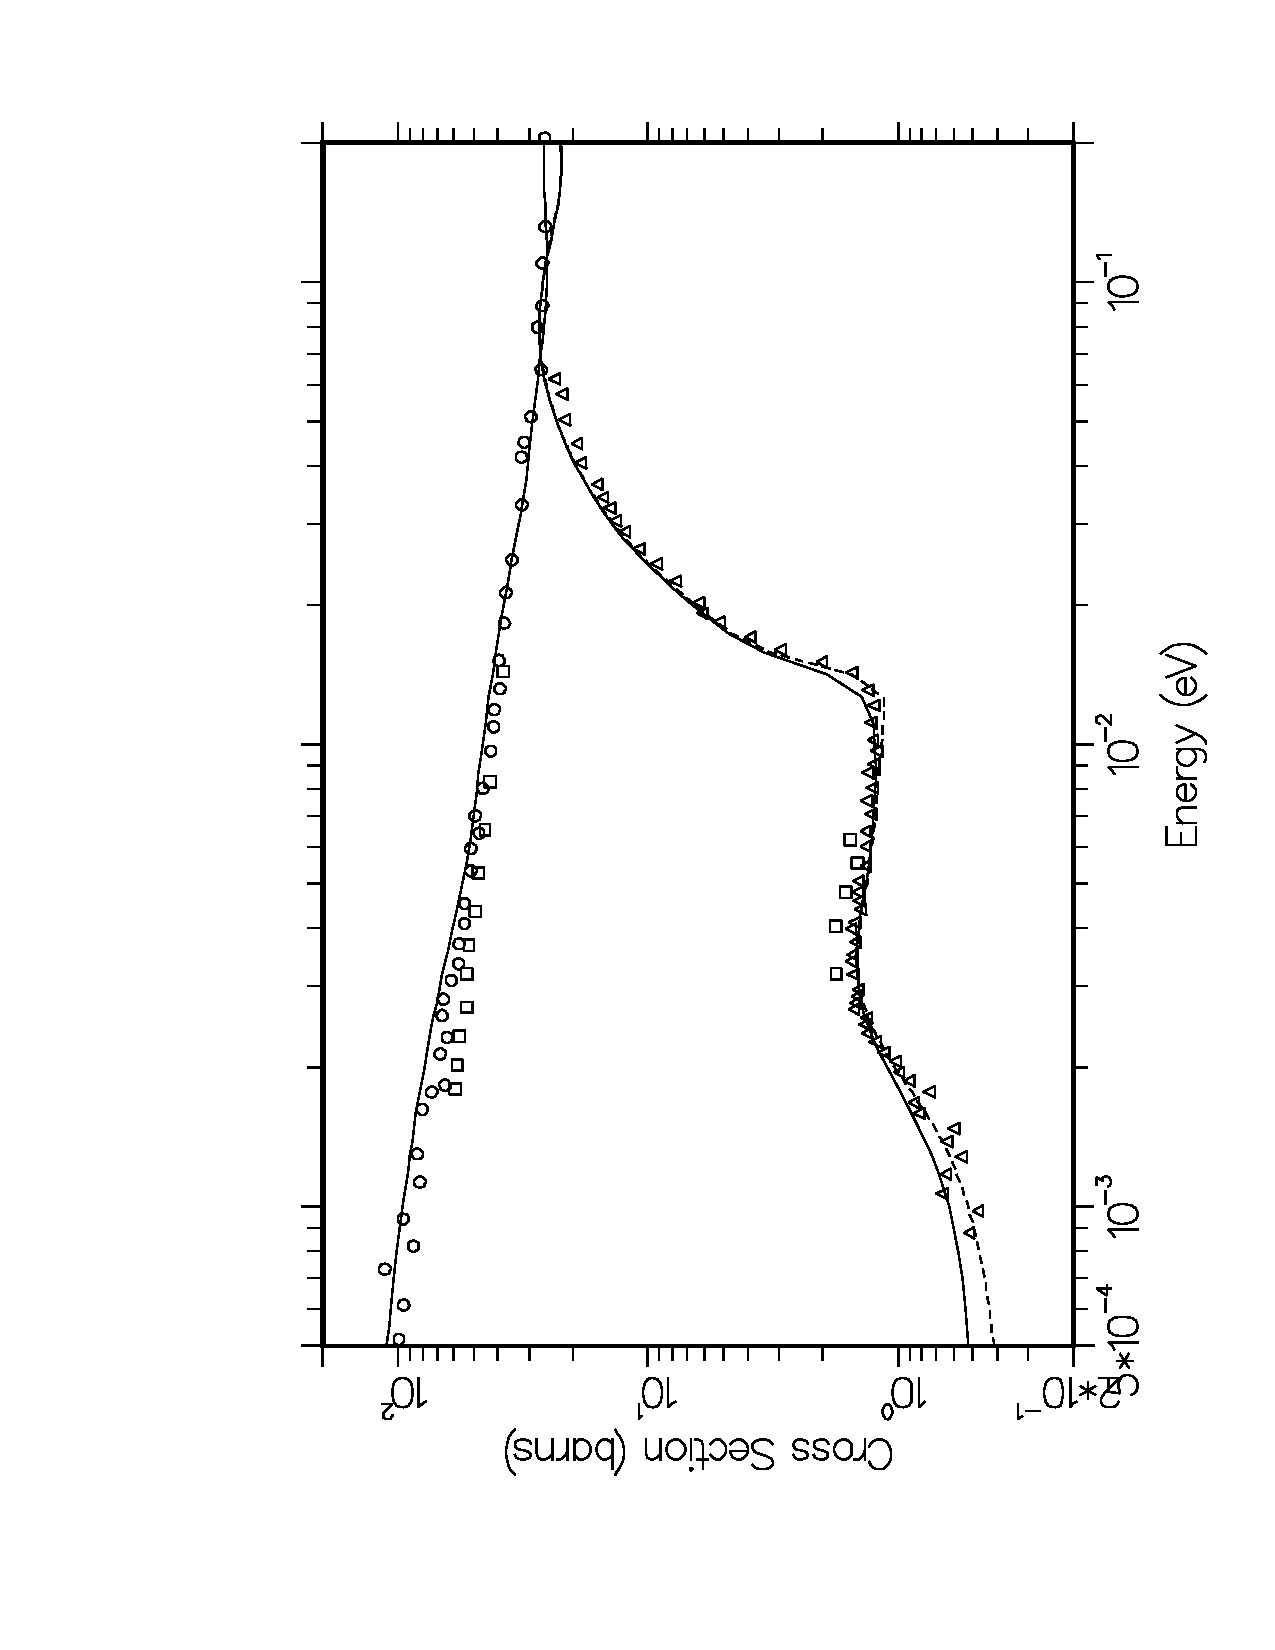
\includegraphics[keepaspectratio, height=3.8in, angle=270]{figs/le15ack}
\caption[Liquid hydrogen cross sections]{The cross sections for liquid
 ortho-hydrogen (upper curve) and liquid para-hydrogen (lower curve)
 at 20K are compared with experimental data\cite{data} due to Squires
 (gas) at 20K (squares), Whittemore at 20K (circles),
 and Seiffert at 14K (triangles).  The solid curves
 are at 20K and the dashed curve is at 14K.  The sharp
 drop in the para cross section below 0.05 eV is due
 to spin coherence, and the second drop below 0.003 eV is due to
 intermolecular interference.}
\label{fig15}
\end{figure}


\subsection{Coding Details}
\label{ssLEAPR_details}

Subroutine \cword{leapr}\index{leapr@{\ty leapr}} is exported by
module \cword{leapm}.  \index{modules!leapm@{\ty leapm}}
It follows the standard pattern for an NJOY module in that it
starts with a group of comment cards describing the code and giving
the input instructions.

LEAPR performs many calculations of exponentials
of very small numbers and of products of small numbers.  These
calculations will lead to underflow conditions on many machines.
These underflow events are not intercepted or reset by LEAPR
for efficiency.  The programmer should use the appropriate
system calls or compiler options to suppress these underflow
messages and to assure that the system does not generate
``Not a Number'' (\cword{NaN}) values that would affect the
calculation.

User input is read in using the standard Fortran READ*. With the
size of the problem determined, storage can be allocated for the
\cword{alpha} grid, the \cword{beta} grid, and the \cword{ssm} and
\cword{ssp} array (if needed).

Most of the main program consists of the loops over principal and
secondary scatterers, and the loop over temperatures.  If the
mixed-moderator option has been requested, the results for the
principal scatterer are written onto a scratch file on unit 10, and the
effective temperature and Debye-Waller factor for the principal
scatterer are stored in the variables \cword{tempf1} and \cword{dwp1}.
The code then loops back to statement 100 to repeat the calculation for
the secondary scatterer.  Note the global variable \cword{arat}.
This is the mass ratio that is used to scale the $\alpha$ grid for
the secondary scatterer in the mixed-moderator calculation.  If only
one scattering law is being calculated, the code drops through to
the ENDF output section.

Inside the temperature loop, LEAPR first reads in the temperature,
the continuous frequency distribution, the oscillator data, and
the pair correlation function.  It then processes the continuous
spectrum by calling subroutine \cword{contin}\index{contin@{\ty contin}},
the translational modes (if any) by calling
\cword{trans}\index{trans@{\ty trans}}, the discrete
oscillators (if any) by calling
\cword{discre}\index{discre@{\ty discre}}, and the liquid
hydrogen or deuterium option using subroutine
\cword{coldh}\index{coldh@{\ty coldh}}.

We next look at \cword{contin}\index{contin@{\ty contin}}. The
first part of the calculation is performed by
\cword{start}\index{start@{\ty start}}, which prepares and
normalizes the functions $\rho(\beta)$ and $P(\beta)$.  It also
calculates the effective temperature and Debye-Waller $\lambda$,
and starts the convolution process for the phonon expansion by
computing ${\cal T}_1$.  The results printed out at this point
refer to the continuous part of the distribution only.  The
effective temperature and Debye-Waller $\lambda$ may change
as other modes are added.

When \cword{start} returns to \cword{contin}, the continuous part of
the scattering law is computed by carrying out the phonon expansion.
At any one time, only ${\cal T}_1$, ${\cal T}_{\rm last}$, and
${\cal T}_{\rm now}$ have to be kept in memory to carry out the
convolution.  Note that the number of elements of ${\cal T}_n$ starts
out equal to the number of $\beta$ values in $\rho$ for $n{=}1$, and then
it increases by this number for every subsequent step. Therefore, the
maximum sizes for \cword{tlast} and \cword{tnow} are equal to the number
of points in the frequency distribution times \cword{nphon}.

Each step of the expansion is handled by the convolution routine
\cword{convol}\index{convol@{\ty convol}}.  The input T arrays
\cword{tlast} and \cword{t1} contain only the $-\beta$
part of the asymmetric T functions.  This is the part that
has the smallest dynamic range, because it is roughly proportional to
the cross section.  Really small numbers like those that occur on the
upscatter side of the asymmetric T function cannot significantly affect
the answers.  This approach was developed to get good results even on
short-word computers that could not represent numbers less than
quantities like $10^{-31}$ or $10^{-45}$.  This is less of a problem
with Fortran-90's ``kind'' method.  Note that \cword{convol}
also returns the quantity \cword{ckk}, which is used to check the
normalization condition on the ${\cal T}_n$.

Returning to \cword{contin}, note that the code determines the maximum
value of $\alpha$ that can be used for each $\beta$ without invoking
the SCT approximation.  This is done by checking each term that is
accumulated into the phonon expansion to see if it is smaller than 0.1\%
of the accumulating ${\cal S}(\alpha,-\beta)$.  These breakpoints are
summarized on the output listing if \cword{iprint}=2.  Next,
\cword{contin} checks the computed scattering law to see if it satisfies
the normalization and sum rule requirements.  The scattering law may
also be printed out by this loop.  Note that the quantity
${\cal S}(\alpha,-\beta)$ is the result actually computed by
\cword{contin}.  The corresponding upscatter side of ${\cal S}$ and
the symmetric $S(\alpha,\beta)$ are computed just for the listing.
On a short-word machine, these two quantities may underflow to zero,
but that doesn't affect the accuracy of subsequent calculations.
The denominator of the normalization test with \cword{sum0} is
$1{-}\exp(-\alpha\lambda)$ because the delta function that represents
the ``zero-phonon'' term is not included in the calculated scattering law.

When \cword{contin} returns to \cword{leapr}, the $-\beta$ side of the
asymmetric scattering law is safely stored in \cword{ssm} for this
temperature.  If translational modes have been requested by entering
a value greater than zero for \cword{twt}, subroutine
\cword{trans}\index{trans@{\ty trans}} is
called.  The task here to to convolve a free-gas or diffusive shape with
the current scattering law.  The approach is to first use
\cword{stable}\index{stable@{\ty stable}}
to compute the free-gas or diffusive shape on an appropriate $\beta$
grid.  Then, subroutine
\cword{sbfill}\index{sbfill@{\ty sbfill}} is called to remap the current
scattering law onto the same $\beta$ grid.  It is then easy to perform
the convolution integral using Simpson's Rule.  The final step is
to add in the convolution of the ``zero-phonon'' term, which is a delta
function, with the translational term.  That step is very easy, because
it is only necessary to interpolate for the translational term at the
current $\beta$ value and multiply by $\exp(-\alpha\lambda)$.  When the
loop over $\beta$ is complete, another $\beta$ loop is used to check
the normalization and sum-rule conditions.  Normally, there is some
loss in accuracy at this point, because it is impractical to keep
the $\beta$ grid fine enough at small $\beta$ to represent the very
sharp shape of the translational contribution at small $\alpha$.
When the $\alpha$ loop is complete, a new value for the effective
temperature to be used with the SCT approximation in computed.
The Debye-Waller $\lambda$ remains unchanged.

The next step is to call subroutine
\cword{discre}\index{discre@{\ty discre}} to add the
contributions from the discrete oscillators, if any.  The keys
to this calculation are the routine
\cword{bfact}\index{bfact@{\ty bfact}}, which generates the terms

\begin{equation}
   \rm e^{-\alpha\lambda_i}\,I_n\left[\frac{\alpha w_i}
     {\beta_i \sinh(\beta_i/2)}\right]\,\rm e^{-n\beta_i/2}\,,
\end{equation}
\vspace{0.5 pt}

\noindent
and the routine \cword{sint}\index{sint@{\ty sint}}, which
interpolates for the scattering law
at $\alpha$ and $\beta{-}n\beta_i$.  \cword{sint} uses the arrays
\cword{bex}, \cword{rdbex}, and \cword{sex}, which are generated
by \cword{bfill}\index{bfill@{\ty bfill}}
and \cword{exts}\index{exts@{\ty exts}}.
These arrays extend the $\beta$ grid
and the $-\beta$ side of the scattering law over the entire $\beta$ range
needed for the discrete oscillator calculation.  This makes it easy for
\cword{sint} to interpolate for the scattering law at a given $\beta$
without having to worry about the asymmetry of the ${\cal S}$ function.
The sum given by

\begin{equation}
   \sum_{n=-\infty}^{\infty} \cdots \,,
\end{equation}
\vspace{0.5 pt}

\noindent
is evaluated by first doing the term with $n{=}0$, then doing the
negative $n$ terms until \cword{add} is less than \cword{tiny}
(currently $1.0\times 10^{-30}$), and finally, doing the positive
$n$ terms until the \cword{add} is less than \cword{tiny}.  This entire
process is continued until all $\beta$ and $\alpha$ values have been
processed.  The normalization and sum-rule checks are carried out as
before.  There is usually some loss in the accuracy of these tests at
high $\alpha$, because the $\beta$ grid doesn't extend to high enough
values to complete the integrals.

New values for the effective temperature and the Debye-Waller
$\lambda$ are also produced by \cword{discre} before it returns
to the main processing line in \cword{contin}.

Subroutine \cword{bfact}\index{bfact@{\ty bfact}}
computes the factors used to weight the various
discrete-oscillator contributions to the scattering law.  The modified
Bessel Functions $I_0(x)$ and $I_1(x)$ are computed separately for
small $x$ and large $x$ to take advantage of the factor $\rm e^{x}$ at
large $x$.  It is easier to control the numerics when $x$ can be
combined with $-\alpha\lambda$ and $-n\beta_i/2$ in the exponent before
computing the factor.  The $I_0(x)$ and $I_1(x)$ are computed using
series expansions; higher orders are generated using reverse
recursion\cite{recipes}.  The numerics of the products $I_n(x)\rm e^{y}$
is controlled to return all significant values for both $+$ and $-n$,
even for large $x$.  This is an improvement over the original LEAP code.

Subroutine \cword{sint}\index{sint@{\ty sint}}
first checks to see if the requested value of $\beta$
is in the tabulated range.  If not, it computes the scattering
law using the SCT expression.  Otherwise, the value is computed by
finding the appropriate panel in the tabulated function and
interpolating on $\log{\cal S}$.  Note that the $\beta$ grid has
been extended over the entire range of negative and positive $\beta$
values using \cword{bfill} and \cword{exts}.

Subroutine \cword{coldh}\index{coldh@{\ty coldh}}
is fairly complicated due to the messy details
of following the quantum mechanics needed to compute the effects of
spin correlation.  It starts by setting values for the atomic masses,
coherent and incoherent scattering lengths.  The fundamental constants
needed are available from the NJOY
\cword{physics} module\index{modules!physics@{\ty physics}}.  It also
sets the translational weight for the free-gas and SCT formulas and
the effective temperature ratio \cword{tbart} for the SCT approximation.
Of course, all these values depend on whether hydrogen or deuterium are
being processed (see \cword{law}).  Inside the $\alpha$ loop, the even
and odd $A$ and $B$ coefficients are computed for the current molecule
from the coherent and incoherent scattering lengths.  The next step is
to prepare the arrays for \cword{sint}, just as was done in \cword{discre}.

The $\beta$ loop is complicated by the fact that it is necessary to keep
both the $+\beta$ and $-\beta$ sides of the scattering function, because
the principle of detailed balance doesn't hold for para or ortho phases
treated separately.  Note that the $+\beta$ terms go into \cword{ssp},
and the $-\beta$ terms go into \cword{ssm}.  For each value of $\beta$,
the sums over the even values of $J'$ and the odd values of $J'$ are
performed separately using \cword{sumh} to retrieve the appropriate sums
over Bessel Functions and Clebsch-Gordan coefficients and using
\cword{sint} to get the corresponding values of the translational
scattering law.  A hidden option is available to use the free-gas law
instead of the scattering law computed from $\rho(\beta)$.  One has to
change the flag \cword{ifree} to 1.

The \cword{endout}\index{endout@{\ty endout}}
routine begins by merging the principal and secondary
scatterer, if the mixed-moderator option was used.  It then
displays the final values of the effective temperatures and Debye-Waller
coefficients.  For comparison with the GA results, the Debye-Waller
terms are printed out as $A\lambda$.  For cases with coherent elastic
scattering, subroutine \cword{coher}\index{coher@{\ty coher}}
is called to construct the Bragg edges.

The routine can now start to build up the output ENDF-6 file.  It starts
by writing the appropriate header cards and the subsection containing
the Hollerith description.  It then constructs a subsection with MF=7
and MT=2 for incoherent elastic scattering, if present.  Note that this
section contains the Debye-Waller integral obtained from \cword{dbw}.
Next, the code constructs a section with MF=7 and MT=2 for coherent
elastic scattering, if present.  Because the Bragg edges get very small
at high energies, it is possible to thin down the coherent-elastic
results slightly.  The fractional tolerance for this thinning
is set to $0.9\times 10^{-7}$.  The final data are output inside a loop
over temperature.  For mixed-moderator cases, the Debye-Waller integral
is computed as the average of the two parts.

The rest of the subroutine outputs the inelastic part.  There are
a number of variations possible.  Normally, the array \cword{ssm}
contains the $-\beta$ side of the asymmetric scattering law.  For
liquid hydrogen or deuterium, \cword{ssm} contains the $-\beta$ side
of the asymmetric scattering law and \cword{ssp} contains the $+\beta$
side.  These numbers have reasonable values, even on short-word machines.
However, the ENDF-6 format normally requires you to give the
``symmetric" $S(\alpha,\beta)$ (it is not really symmetric for
liquid hydrogen or deuterium).  This function can require that numbers
on the order of $10^{-50}$ be kept, if incident energies as high as 4 eV
are needed.  For cold moderators, it is necessary to handle numbers on
the order of $10^{-99}$.  For NJOY2016, this is handled by using the
Fortran-90 ``kind'' mechanism.

\subsection{Error Messages}
\label{ssLEAPR_msg}

\begin{description}
\begin{singlespace}

\item[\cword{error in sjbes***argument is invalid...}] ~\par
  There is a problem with the argument to the Bessel functions used
  for cold hydrogen and deuterium calculations.

\item[\cword{message from sjbes---value is not accurate...}] ~\par
  There is a problem with calculating the Bessel functions.

\item[\cword{error in coh***illegal lat}] ~\par
  Currently limited to 1 to 6, for graphite, be, and beo,
  al, pb, and fe, respectively.

\item[\cword{error in coh***storage exceeded}] ~\par
  Currently limited to \cword{maxb}=60 000, the size of the allocatable
  array \cword{bragg} in subroutine \cword{leapr}.

\item[\cword{error in endout***scratch storage exceeded for hollerith...}] ~\par
  This refers to the allocatable array \cword{scr} with length
  \cword{mscr}=4000 in subroutine \cword{leapr}.

\end{singlespace}
\end{description}

\cleardoublepage

